\documentclass{book}
\usepackage{graphicx} % Required for inserting images

\usepackage[utf8]{inputenc}
\usepackage[T1]{fontenc}
\usepackage{listings}
\usepackage{appendix}
\usepackage{siunitx}
\usepackage{multirow}
\usepackage{mhchem}
\usepackage{natbib}
\usepackage{booktabs}
\usepackage{bachelorstitlepageUNAM}
\usepackage[spanish,es-nodecimaldot,es-tabla]{babel}
\usepackage{tikz} 
\usepackage{tocloft}
\graphicspath{{./figs/}}
\usepackage{setspace}
\usepackage{hyperref}

\DeclareSIUnit\msun{\text{M\ensuremath{_\odot}}}
\usepackage{astrojournals}
\bibliographystyle{aasjournal}
\renewcommand{\lstlistingname}{Algoritmus}

\title{Avances de tesis}
\author{r.reyes }
\date{December 2023}

\begin{document}

    \begin{titlepage}
        \thispagestyle{empty}
        \begin{minipage}[c][0.17\textheight][c]{0.25\textwidth}
            \begin{center}
                
\includegraphics[width=3.5cm, height=3.5cm]{Escudo-UNAM.pdf}
            \end{center}
        \end{minipage}
        \begin{minipage}[c][0.195\textheight][t]{0.75\textwidth}
            \begin{center}
                \vspace{0.3cm}
                \textsc{\large Universidad Nacional Aut\'onoma de M\'exico}\\[0.5cm]
                \vspace{0.3cm}
                \hrule height2.5pt
                \vspace{.2cm}
                \hrule height1pt
                \vspace{.8cm}
                \textsc{Instituto de Radioastronomía y astrofísica}\\[0.5cm] %
            \end{center}
        \end{minipage}

        \begin{minipage}[c][0.81\textheight][t]{0.25\textwidth}
            \vspace*{5mm}
            \begin{center}
                \hskip2.0mm
                \vrule width1pt height13cm 
                \vspace{5mm}
                \hskip2pt
                \vrule width2.5pt height13cm
                \hskip2mm
                \vrule width1pt height13cm \\
                \vspace{5mm}
                
\includegraphics[height=4.0cm]{logoIRyAnegro_1.png}
            \end{center}
        \end{minipage}
        \begin{minipage}[c][0.81\textheight][t]{0.75\textwidth}
            \begin{center}
                \vspace{1cm}

                {\large\scshape El impacto del viento estelar y la radiación en glóbulos neutros alrededor de una estrella Wolf-Rayet}\\[.2in]

                \vspace{2cm}            

                \textsc{\LARGE T\hspace{1.5cm}E\hspace{1.5cm}S\hspace{1.5cm}I\hspace{1.5cm}S}\\[0.5cm]
                \textsc{\large que para obtener el grado de:}\\[0.5cm]
                \textsc{\large Maestro en ciencias (astrofísica)}\\[0.5cm]
                \textsc{\large presenta:}\\[0.5cm]
                \textsc{\large {Roberto Reyes Cabañas}}\\[2cm]          

                \vspace{0.5cm}

                {\large\scshape Tutor:\\[0.3cm] {Dr. William John Henney }}\\ [.2in]

                \vspace{0.5cm}

                \large{Morelia, Michoacán,}{ }{2024}
            \end{center}
        \end{minipage}
    \end{titlepage}

%\maketitle

\chapter*{Resumen}

La nebulosa circunestelar M1-67 alrededor de la estrella Wolf-Rayet WR~124 contiene cientos de pequeños glóbulos neutros, como revelan imágenes recientes del JWST. La emisión ionizada de la nebulosa muestra un patrón intrincado de cáscaras y filamentos, muchos de los cuales parecen asociados con los glóbulos pero desplazados hacia la estrella central. Proponemos un modelo simple para la nebulosa en el que los flujos de fotoevaporación desde la superficie irradiada de los glóbulos interactúan con el viento estelar de la estrella Wolf-Rayet para formar cáscaras de emisión hemisféricas. Probamos este modelo contra imágenes del JWST y H alpha del HST de la nebulosa, encontrando una buena concordancia para los glóbulos mejor observados y más aislados. El modelo proporciona una explicación física para la morfología observada de la nebulosa y los glóbulos, y sugiere que los glóbulos están protegidos hidrodinámicamente del viento estelar por los flujos de fotoevaporación. Derivamos una estimación independiente de la fuerza del viento estelar, que es consistente con valores previamente derivados de la modelación de la atmósfera estelar. También somos capaces de restringir la distribución tridimensional de los glóbulos.

\newpage

\tableofcontents

\newpage

\chapter{Introducción}

Los \text{glóbulos} son grandes concentraciones de gas y polvo en el medio interestelar que se cree que se forman por inestabilidades térmicas, colapso gravitacional o turbulencia. Estos glóbulos se pueden formar en regiones de formación estelar masiva o en nebulosas alrededor de estrellas evolucionadas.

En general los glóbulos tienen una gran variedad de tamaños. Por ejemplo cuando nos referimos a los glóbulos en regiones de formación estelar masiva, estos tienden a ser de un gran tamaño comúnmente, $\sim$\SI{0.1}{pc}, e interactúan con la radicación UV (ultravioleta) de las estrellas jóvenes masivas como estrellas tipo O, mientras que en nebulosas alrededor de estrellas evolucionadas son de un tamaño más pequeño, $\sim$\SI{e-2}{pc}. En algunos casos dependiendo que tan intensa es la radiación incidente por parte de la o las estrellas, podemos ver un \textit{flujo fotoevaporativo} por parte del glóbulo, el cual es causado por la radiación incidente.

Los primeros glóbulos fueron observados por Bart Bok en 1940, estos glóbulos son nubes oscuras, relativamente pequeños comparados con otras regiones de formación estelar, que tienen gran cantidad de gas y polvo. Estos glóbulos contienen principalmente hidrógeno molecular en su interior, así como también pueden tener otras moléculas, metales e incluso algunos silicatos. Si bien puede tener formación estelar en su interior no podemos ver la radiación de las estrellas ya que es absorbida por el hidrógeno atómico y el polvo, es por eso que se ven oscuras. Sin embargo, estos pueden ser radiados externamente, en regiones de formación estelar, por estrellas jóvenes masivas que se están formando cerca, y en algunos casos podemos ver el frente de ionización.

\begin{figure}[h!]
    \centering
    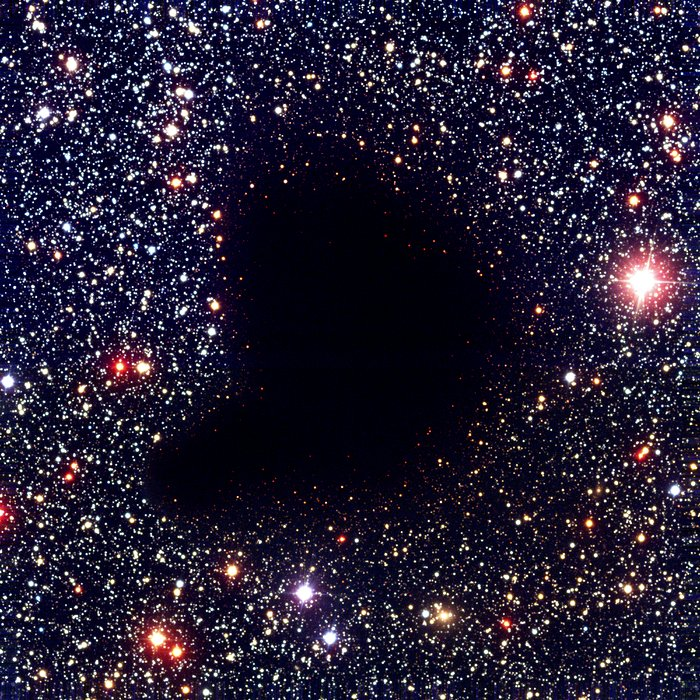
\includegraphics[width=0.75\textwidth]{images Chapter 1/C1_Bok_globule.jpg}
    \caption{Imagen de Banard 68, un ejemplo de un glóbulo de Bok, visto con Very Large Telescope FORS1 en 440 nm, 557 nm y 768 nm. Se puede apreciar una zona oscura y lo que pareciera ser enrojecimiento de las estrellas por polvo en la superficie del glóbulo. En esta imagen podemos ver que no hay evidencia de alguna fotoevaporación externa por parte de estrellas. \citep{Alves:2001}.}
    \label{fig:Banard}
\end{figure}

Esta interacción entre estrellas y glóbulos se puede dar a diferentes escalas, lo que nos da una gran variedad de estructuras. Entre las de mayor tamaño se encuentran lo que parecen ser columnas, pilares o trompas de elefantes, como se les conoce en la literatura, que llegan a tener un tamaño de $\sim$\SI{1}{pc} y una densidad del orden de \SI{e3}{cm^{-3}}. Comúnmente se le suele llamar glóbulo a aquellos que tienen tamaños semejantes a la de los pilares o columnas pero son más densos, $\sim$ \SI{e4}{cm^{-3}}. Esta interacciones también se puede dar dentro de regiones HII, como vemos en la figura \ref{fig:Pillars}.

\begin{figure}[h]
    \centering
    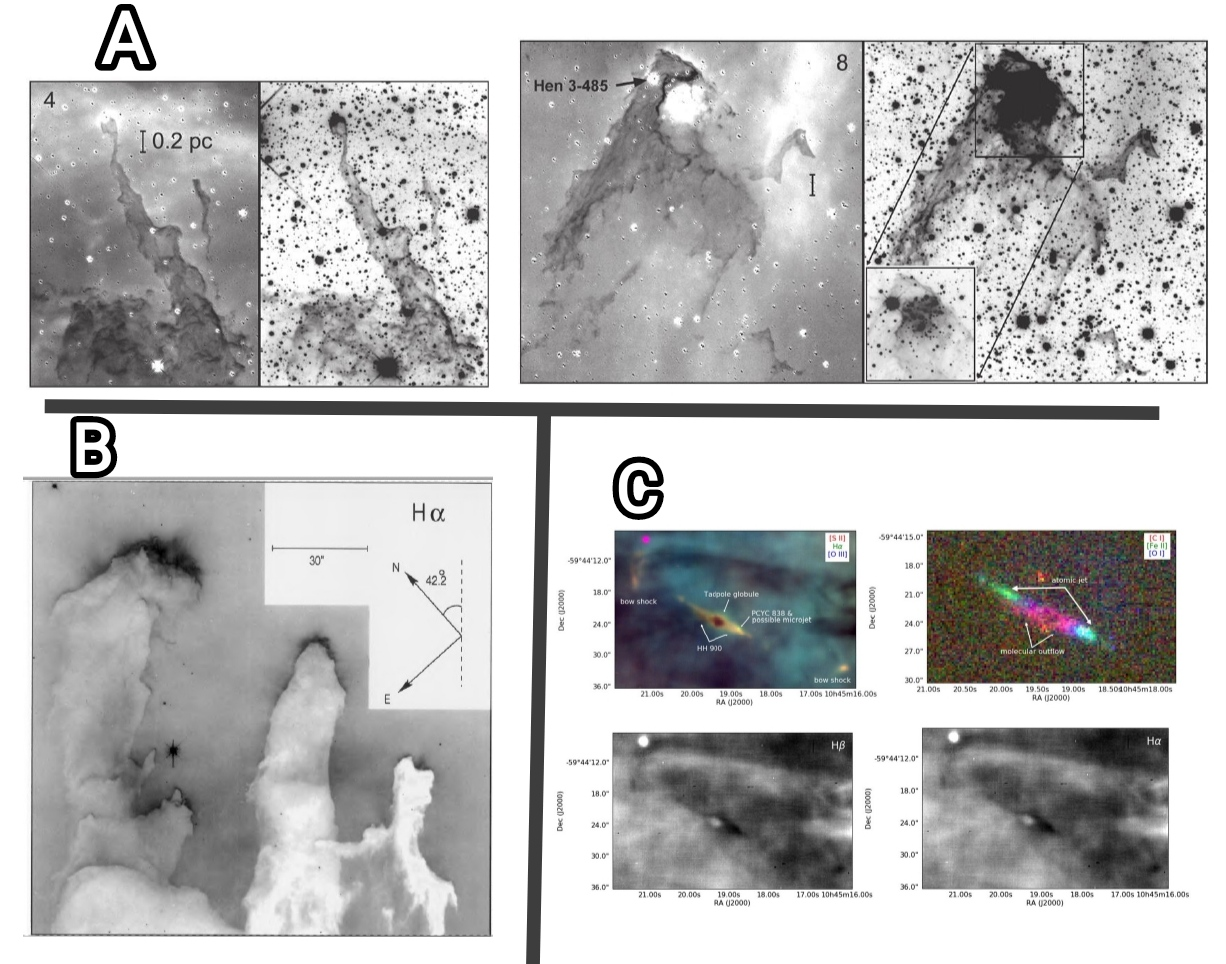
\includegraphics[width=1 \textwidth]{images Chapter 1/C1_Pillars.jpg}
    \caption{En \textbf{A} vemos dos ejemplos de pilares, donde la imagen derecha de cada ejemplo es vista a \SI{2.12}{\mu m} (\SI{}{H_2}) y la imagen izquierda es \SI{}{H_2-Br_{\gamma}} \citep{Hartigan:2015}. \textbf{B} es un ejemplo de una trompa de elefante, es una imagen de M16 tomada con WFPC2 con e filtro F656N, los \SI{30}{\arcsecond} corresponden \SI{9e17}{cm} (\SI{0.29}{pc}) \citep{JJHester:1996}. \textbf{C} es el outflow de Tadpole globule, el cual consta del sistema HH900 jet+outflow, la imagen de abajo es vista en \SI{}{H_\alpha} con el continuo 
    \citep{MeganReiter:2019}. }
    \label{fig:Pillars}
\end{figure}

En escalas más pequeñas están lo que se conoce como EGGs (Evaporating Gaseous Globule) los cuales tienen tamaños de $\sim$\SI{0.1}{pc}, y los proplyds que tienen tamaños $\le\SI{e-2}{pc}$. 


Estos glóbulos no están solo en regiones de formación estelar, como ya hemos dicho, también hay dentro de nebulosas alrededor de estrellas evolucionadas donde se les conoce más comúnmente como \textit{nudos}, un ejemplo de esto es la imagen \textbf{D} de la figura \ref{fig:nudos}. Estos nudos son los que estudiaremos más fondo en este trabajo.

\begin{figure}[h]
    \centering
    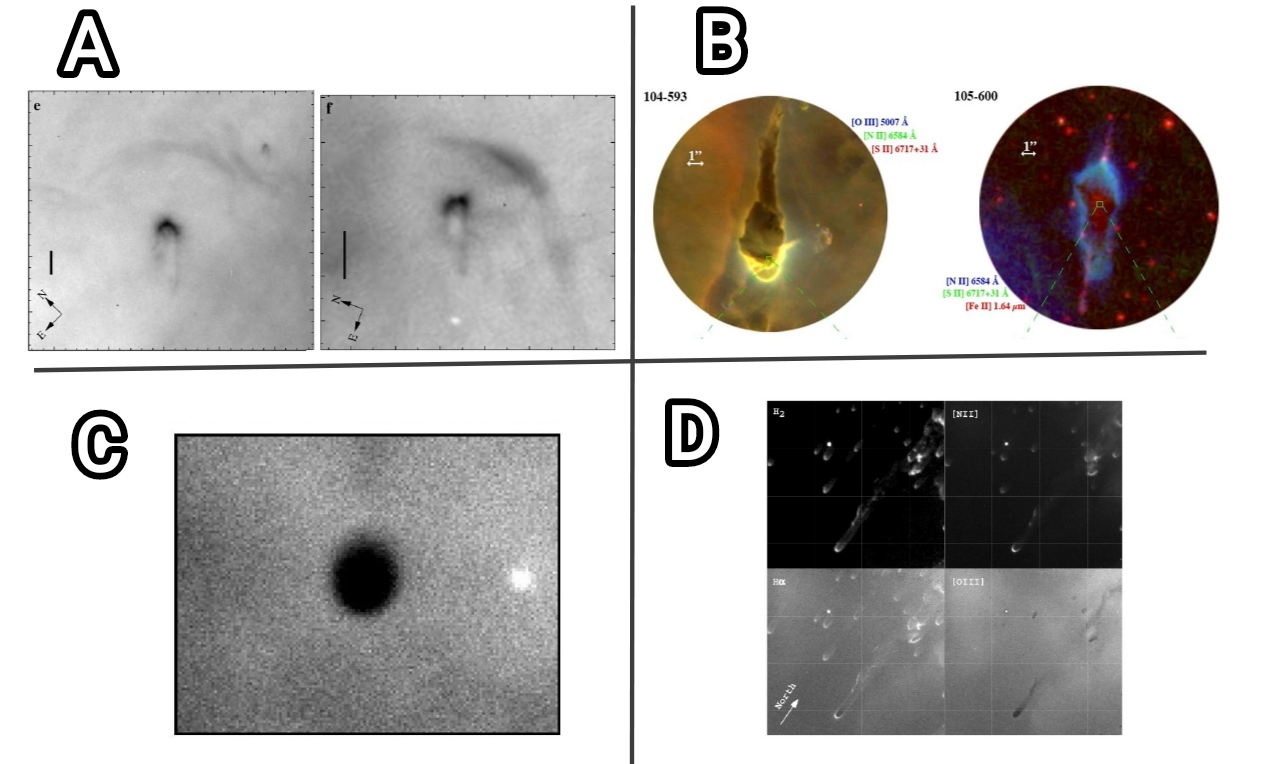
\includegraphics[width=1 \textwidth]{images Chapter 1/C1_Globulettes.jpg}
    \caption{En \textbf{A} vemos proplyds con su bowshock en Orion tomado con HST planetary camera, la barra negra indica una medida de \SI{1}{\arcsecond} que corresponde a 430 AU (\SI{2e-3}{pc}) \citep{Garcia-Arredondo:2001}. \textbf{B} son ejemplos de EGGs en Carina, tomado con WFC3, ACS, WFPC2 \citep{Mesa-Delgado:2016}. \textbf{C} es el globulette denso RN88 visto en \SI{}{H_\alpha} con un diámetro de \SI{6}{\arcsecond} (\SI{4e-2}{pc}) en la nebulosa de Rosette \citep{GFGahm:2013}. \textbf{D} son ejemplos de nudos en la nebulosa de la Hélice, los mosaicos tienen una medida de \SI{47.5}{\arcsecond}$\times$\SI{44.8}{\arcsecond} (\SI{4.76e-2}{pc}$\times$\SI{4.49e-2}{pc}) \citep{O'Dell:2007}. }
    \label{fig:nudos}
\end{figure}



\section{Flujos de foto evaporación ionizada} \label{Sec:fluijos fotoevaporativos}

Todos los ejemplos de las figuras \ref{fig:Banard}, \ref{fig:Pillars} y \ref{fig:nudos} se encuentran ya sea en regiones de formación estelar o en nebulosas alrededor de estrellas evolucionadas. 

Lo interesante en todos estos ejemplos es la forma que toman al interaccionar con las estrellas más masivas que se encuentran cerca, esto para los glóbulos que se encuentran en regiones de formación estelar.  Mientras que los que se encuentran en nebulosas planetarias interactúan con la estrella evolucionada. Durante estas interacciones en algunos casos podemos ver lo que se conoce como flujos fotoevaporativos, los cuales explicaremos mejor a continuación.

Para que se pueda dar esta interacción y crear un flujo fotoevaporativo por parte de la nube es necesario que la estrella ionizante sea masiva o tenga un gran flujo ionizante como para poder ionizar el gas neutro. \cite{OortySpitzer_1955} explican a manera detallada como es la interacción entre una estrella tipo O y una nube interestelar de gas neutro. Con esto podemos explicar de una mejor manera como es la interacción en regiones de formación estelar masiva. Recordemos que en las regiones de formación estelar hay muchas estrellas nuevas que emiten principalmente en radio o infrarrojo, por lo que no todas las estrellas nuevas pueden ionizar el gas neutro.

\cite{OortySpitzer_1955} consideran tres partes importantes para esto, la estrella ionizante, la nube interestelar de gas neutro y la región que hay entre la estrella y la nube interestelar. La nube interestelar debe ser mucho más densa y fría que la región que hay entre la estrella y la nube como vemos en la figura \ref{kahn_zones}.

\begin{figure}[h]
    \centering
    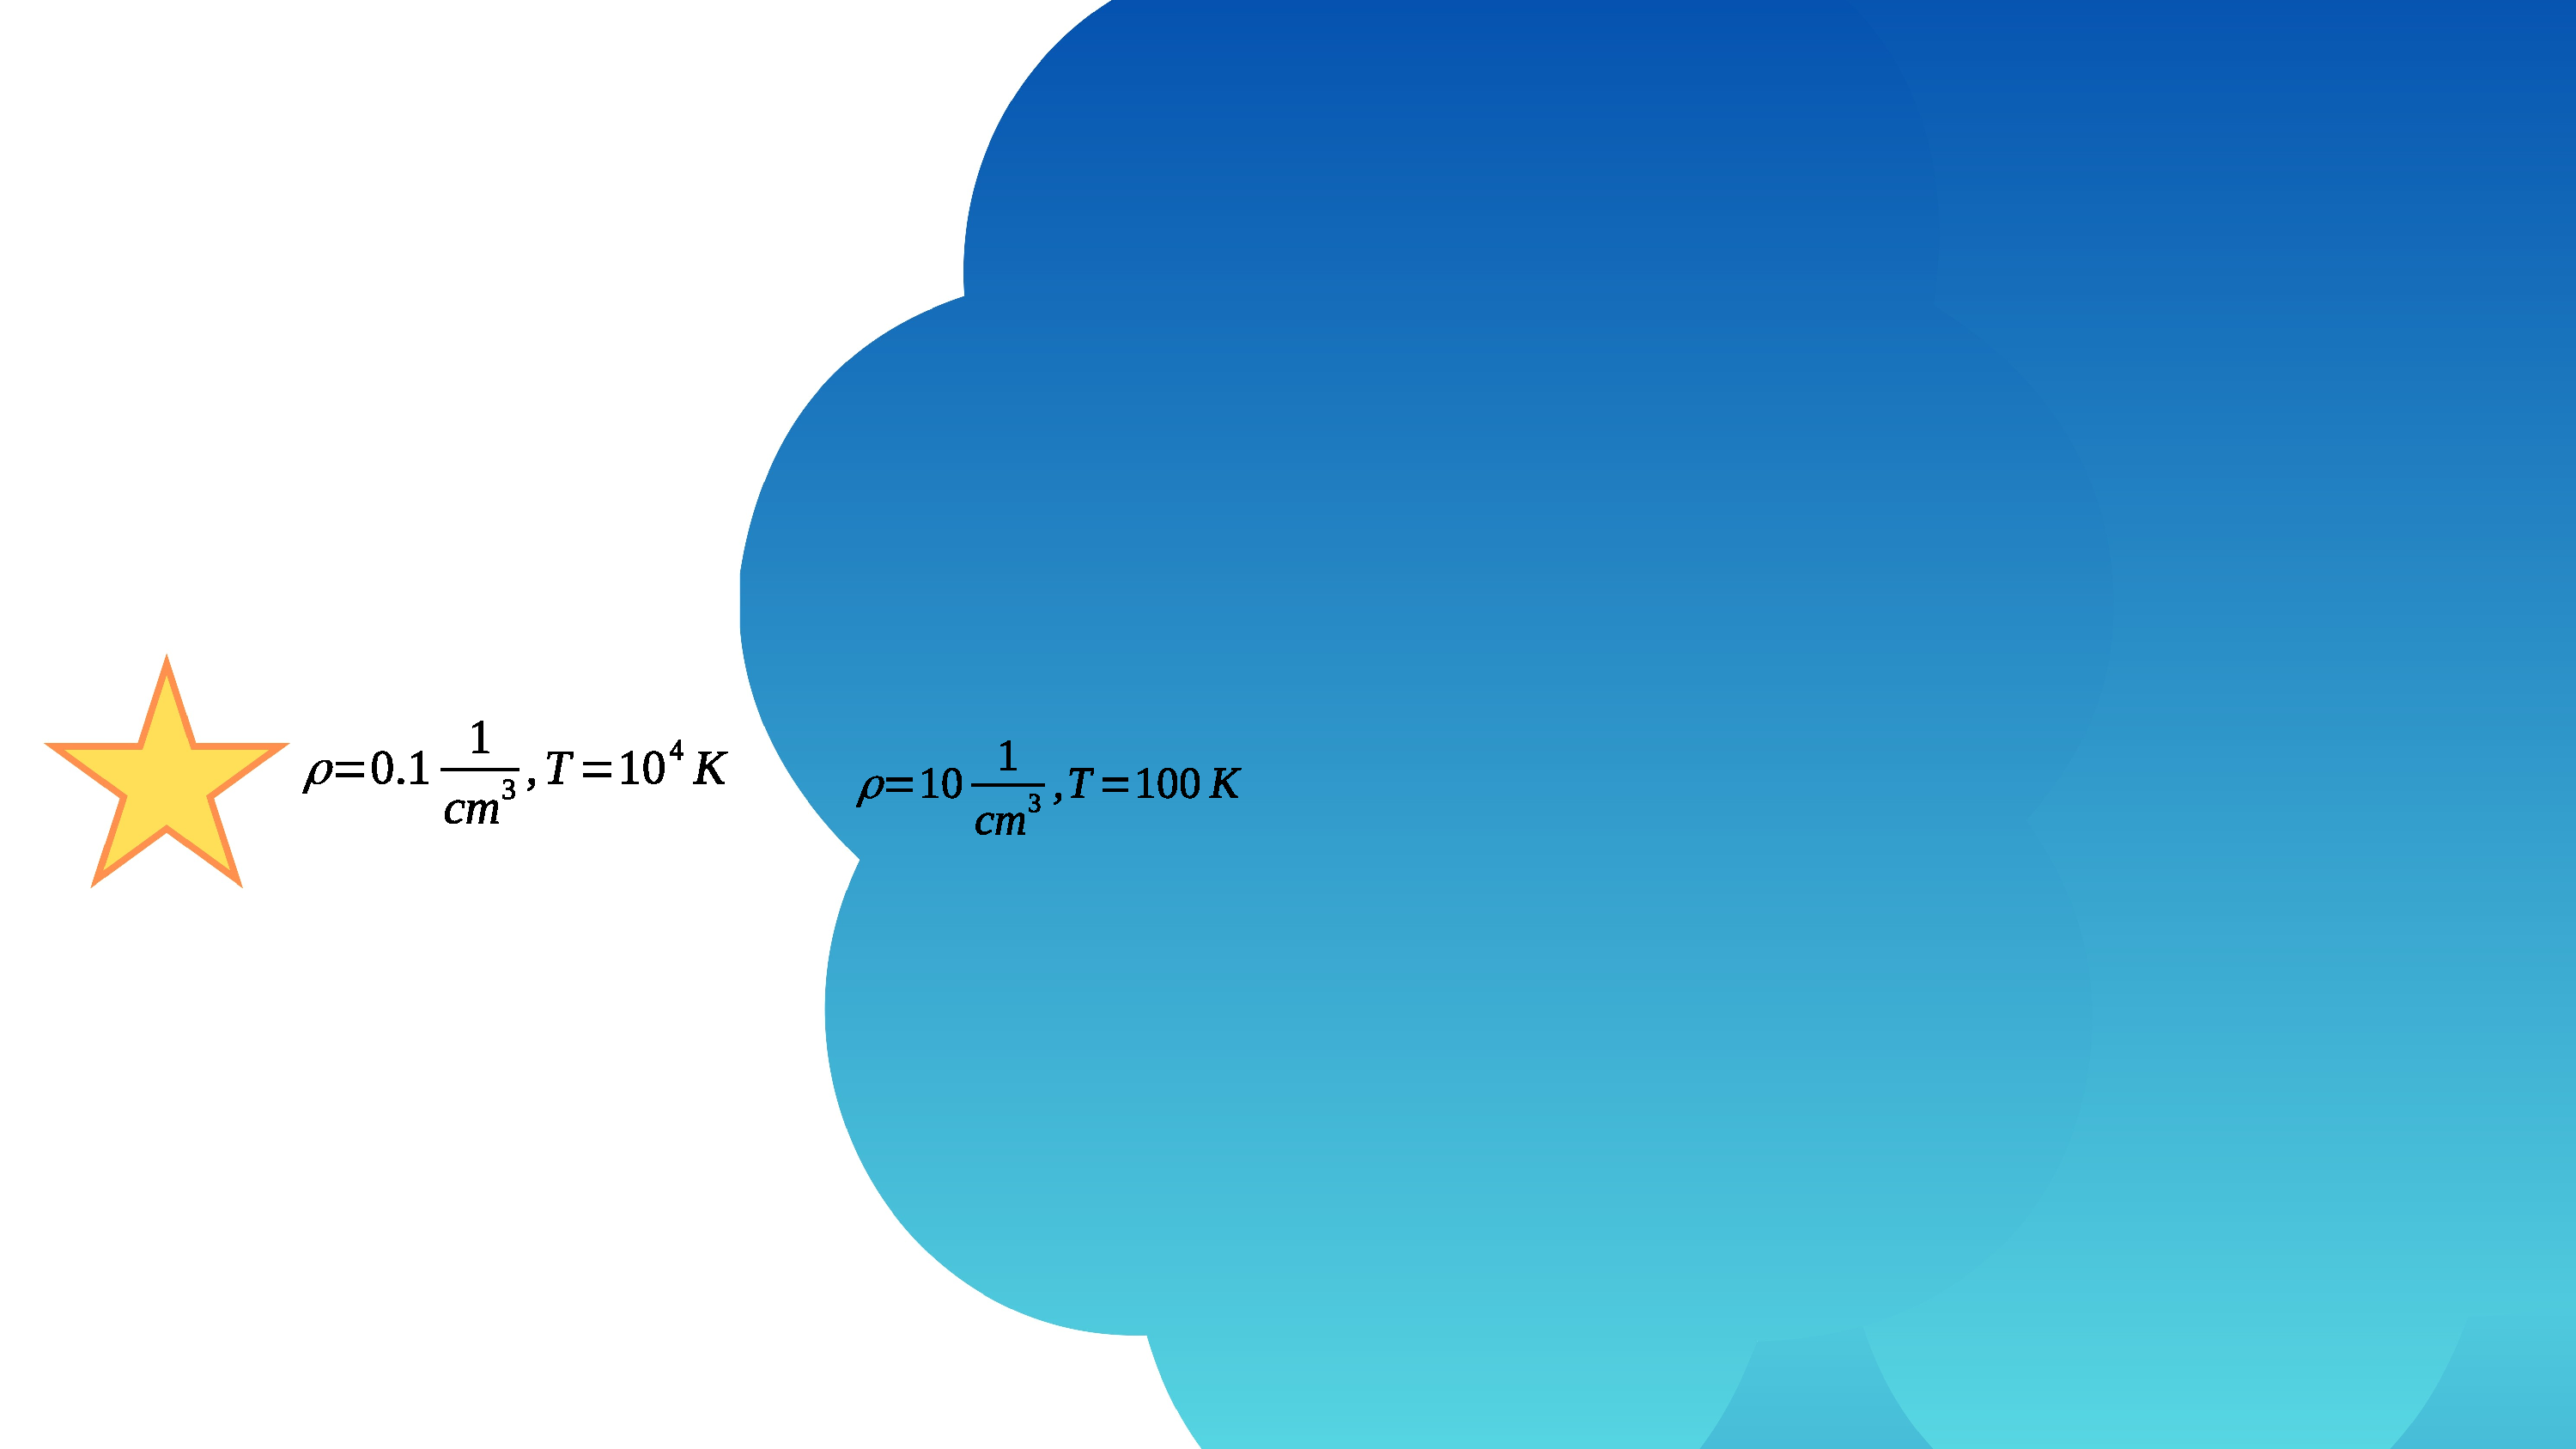
\includegraphics[width= \textwidth]{artesanales/ImgFi01-5.pdf}
    \caption{Esquema inicial utilizado en \cite{Kahn:1954}}
    \label{kahn_zones}
\end{figure}

Cuando la radiación UV comienza a calentar el gas de la nube, el gas ionizado comienza a expandirse en dirección a la estrella, esto ya que en esta dirección la densidad es menor que la de la nube y puede expandirse libremente. 

En un inicio esta radiación ioniza el gas a una tasa muy rápida causando una ``tormenta de partículas ionizantes'' que viene por parte de la nube, conforme esto va evolucionando se crea una capa aislante alrededor de la nube. Esta radiación produce un choque ionizante lo cual provoca que la nube se comprima. También se produce un frente de ionización que avanza hacia la nube haciendo que esta se vaya alejando de la estrella. Mientras esto ocurre hay un choque interno que va viajando a través de la nube a la parte trasera \citep{Bertoldi_1989}. Para que esto ocurra \cite{Kahn:1954} da cierto criterios, en los cuales dice que la radiación no debe ser muy débil o demasiado fuerte.

\section{Estrellas Wolf-Rayet y sus vientos}

Las estrellas WR (Wolf-Rayet) son estrellas evolucionadas de estrellas masivas, como estrellas tipo O, que tienen una alta pérdida de mas debido a sus grandes vientos y fueron nombradas así después de que Charles Wolf y Georges Rayet identificaran 3 estrellas en Cygnus con sus  anchas líneas de emisión que las caracterizan muy bien. 

Estas estrellas se caracterizan principalmente por sus fuertes vientos que pueden ser del orden de $\sim$\SI{1000}{km/s}, los cuales provocan sus líneas de emisión anchas. Así como también tienen una alta pérdida de masa $\sim$2--\SI{10e-5}{\msun/yr}. Típicamente son estrellas de 10--\SI{25}{\msun} que son descendientes de estrellas tipo O y se caracterizan por tener intensas líneas de emisión de libre-libre desde el $\mu$m hasta el cm \citep{crowther:2007}.

A estas estrellas se les clasifica por el cociente que hay entre sus líneas de emisión intensa que las caracterizan. \cite{Smith:1968} las clasifica principalmente como WN a aquellas que son abundantes en He y N, WC a las que son abundantes en He y C. Además les pone un número para identificar esencialmente si son tipo tardío o temprano.

\begin{table}[h!]
    \begin{center}
        \begin{tabular}{c c}
        \toprule
        \multicolumn{2}{c}{Clasificación de estrellas WR} \\ \midrule
        Índice espectral    & Tipo de estrellas\\ \midrule
        WN2--5     & Tipo temprana, WNE (Early WN)\\
        WN7--9 & Tipo tardía, WNL (Late WN) \\
        WC4--6 & WCE\\
        WC7--9 & WCL \\ \bottomrule
        \end{tabular}
    \caption{Principal clasificación de estrellas WR  según sus líneas de emisión. Dentro de las WC, las que se clasifican como WC6 pueden ser de tipo tardía o temprana.}
    \label{tab:WR-clasificacion}
    \end{center}
\end{table}

También están las estrellas WO que son abundantes en He y O, pero en realidad son una extensión de las WCE. Para las estrellas en las que detectamos una cantidad considerable de H en su atmósfera se les pone también una ``h'' \citep{SSM:1996}.

Debido a que no se han encontrado muchas estrellas WR se les suele asociar un número pero este número no tiene nada que ver con su índice espectral.

\section{Nebulosa M1-67}

M1-67 es la nebulosa alrededor de la estrella WR-124, que tiene índice espectral WN8h. En la figura \ref{fig:nudos WR124} vemos que la imagen tomada con el telescopio espacial Hubble (HST) en \unit{H\alpha} se puede notar una gran presencia de H en toda la nebulosa, mientras que en la imagen tomada por el telescopio espacia James Webb (JWST), tomada en varios filtros de los cuales incluye  el infrarrojo cercano, podemos ver una gran estructura. Algo muy notorio a simple vista en la imagen de JWST es que podemos apreciar la presencia de algunos nudos en la nebulosa como se ve  en la figura \ref{fig:nudos WR124}.

\begin{table}[h]
    \centering
    \begin{tabular}{c c c}
        \toprule
        \multicolumn{3}{c}{Parámetros de la estrella WR 124} \\ \midrule
         D & \SI{5.429}{kpc} & J. Arthur, priv.~comm.\\
         $v_\infty$ & \SI{710}{km/s}  & \cite{Hamman:2006}\\
         $\dot{M}$ & \SI{2e-5}{M_\odot/yr} & ?\\
         $S_*$ & \SI{1.25e49}{s^{-1}} & \cite{crowther:2007}  \\
         $F_{H_\alpha}$ & \SI{3e-14}{erg.cm^{-2}.s^{-1}} & \cite{Grosdidier:1998}\\ \bottomrule
    \end{tabular}
    \caption{Parámetros de WR 124}
    \label{tab:parametros WR-124}
\end{table}

\begin{figure}[h]
    \centering
    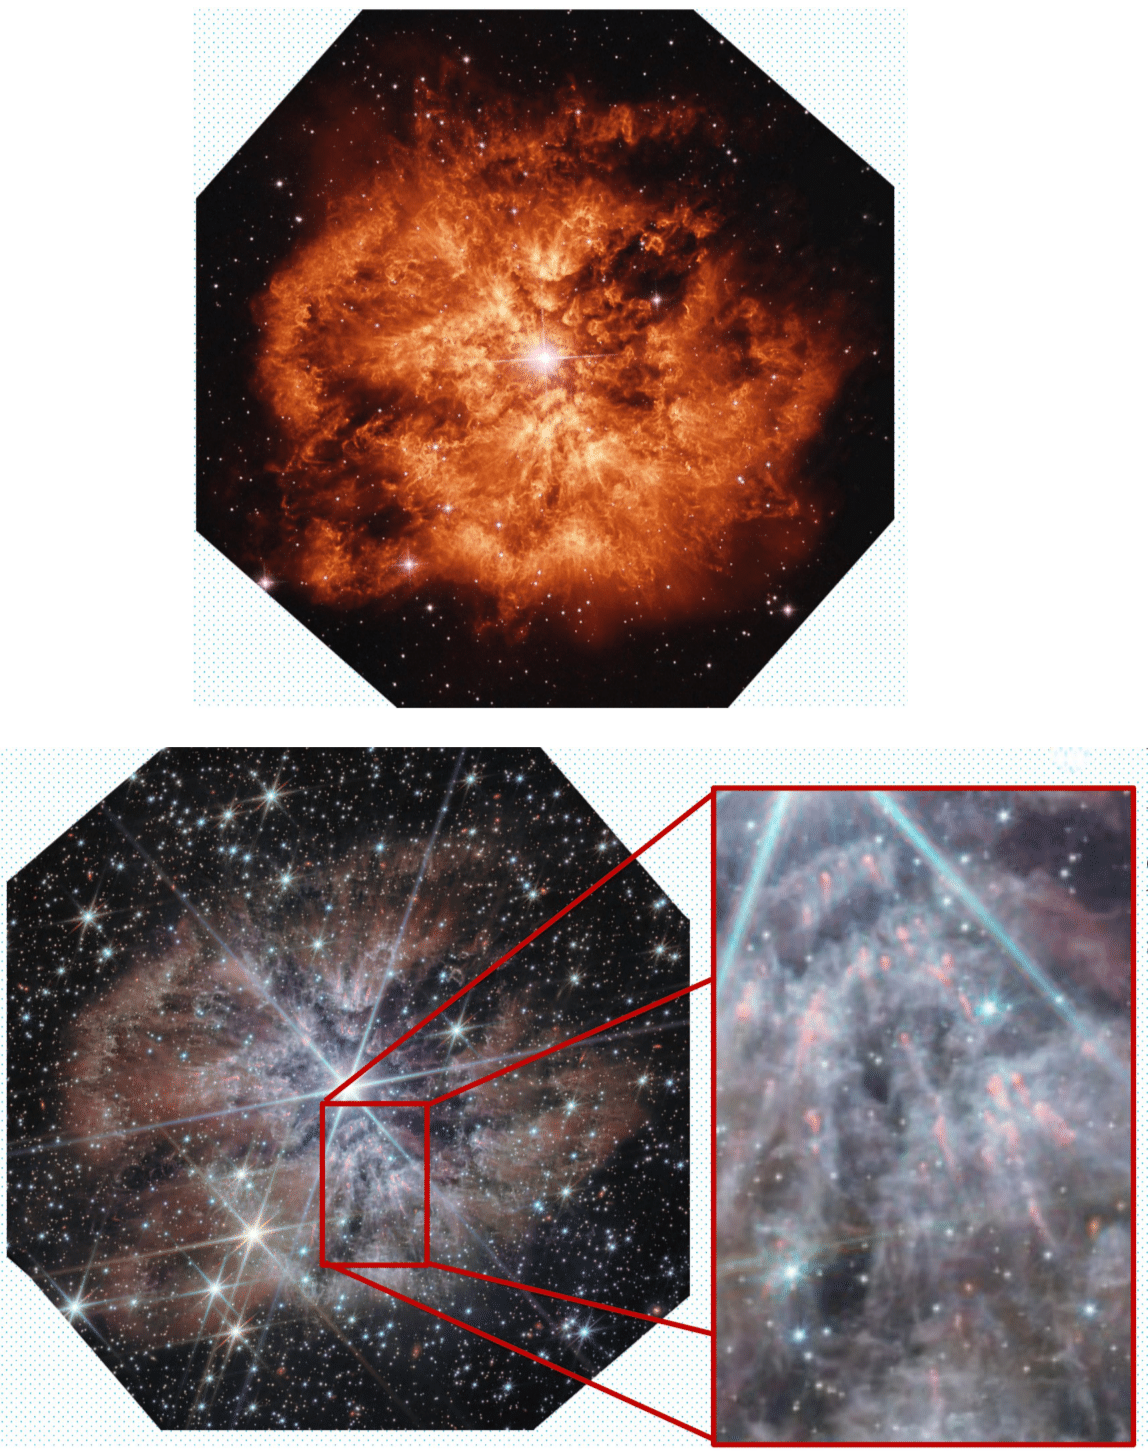
\includegraphics[width=\textwidth]{images Chapter 1/c1WR.png}
    \caption{En la imagen de arriba vemos la nebulosa M1-67 con el filtro \unit{H\alpha} visto con la cámara WFPC2 del HST mientras que en la imagen de abajo a la izquierda es con los filtros F444W, F335M, F210M, F150W, F090W usando la NIRcam del JWST y a su derecha un zoom en una región donde podemos ver mejor estos nudos en la nebulosa. Vemos como el color rosa, la emisión de PAHs, nos muestra mejor como podría ser la morfología del gas neutro y en gris lo que parece ser su interacción con la estrella y su viento estelar.}
    \label{fig:nudos WR124}
\end{figure}

La presencia de estos nudos se puede ver en toda la nebulosa. Algunos de estos nudos se encuentran en grupos y con distintas morfologías. 

\chapter{Modelos analíticos de flujos fotoevaporativos interactuando con una presión externa}
\chaptermark{Modelo analítico}

En este capítulo vamos a describir el modelo que se propone para explicar la interacción que hay entre el flujo fotoevaporativo por parte de los nudos que hay en la nebulosa M1-67 y el viento estelar por parte de la estrella WR-124. Para esto hemos considerado que ya han pasado todas las fases mencionadas en la sección \ref{Sec:fluijos fotoevaporativos} y ahora estamos en un equilibrio de ionización, los nudos no se comprimirán o expandirán en escalas significativas, es decir, que podemos considerar que el tamaño del nudo será constante. Podemos apreciar mejor la presencia de estos nudos en la figura \ref{fig:nudos WR124}.

En esta interacción entre el flujo fotoevaporativo, el cual es supersónico, y el viento estelar se producen dos zonas chocadas y entre estas dos zonas una discontinuidad de contacto como se describe en la figura \ref{fig:zones}. De estas zonas esperamos ver solo el flujo fotoevaporativo chocado y no el viento estelar chocado ya que este último es menos denso además de que es no radiativo y la longitud de enfriamiento es más grande que la región de interacción

\begin{figure}[h]
    \centering    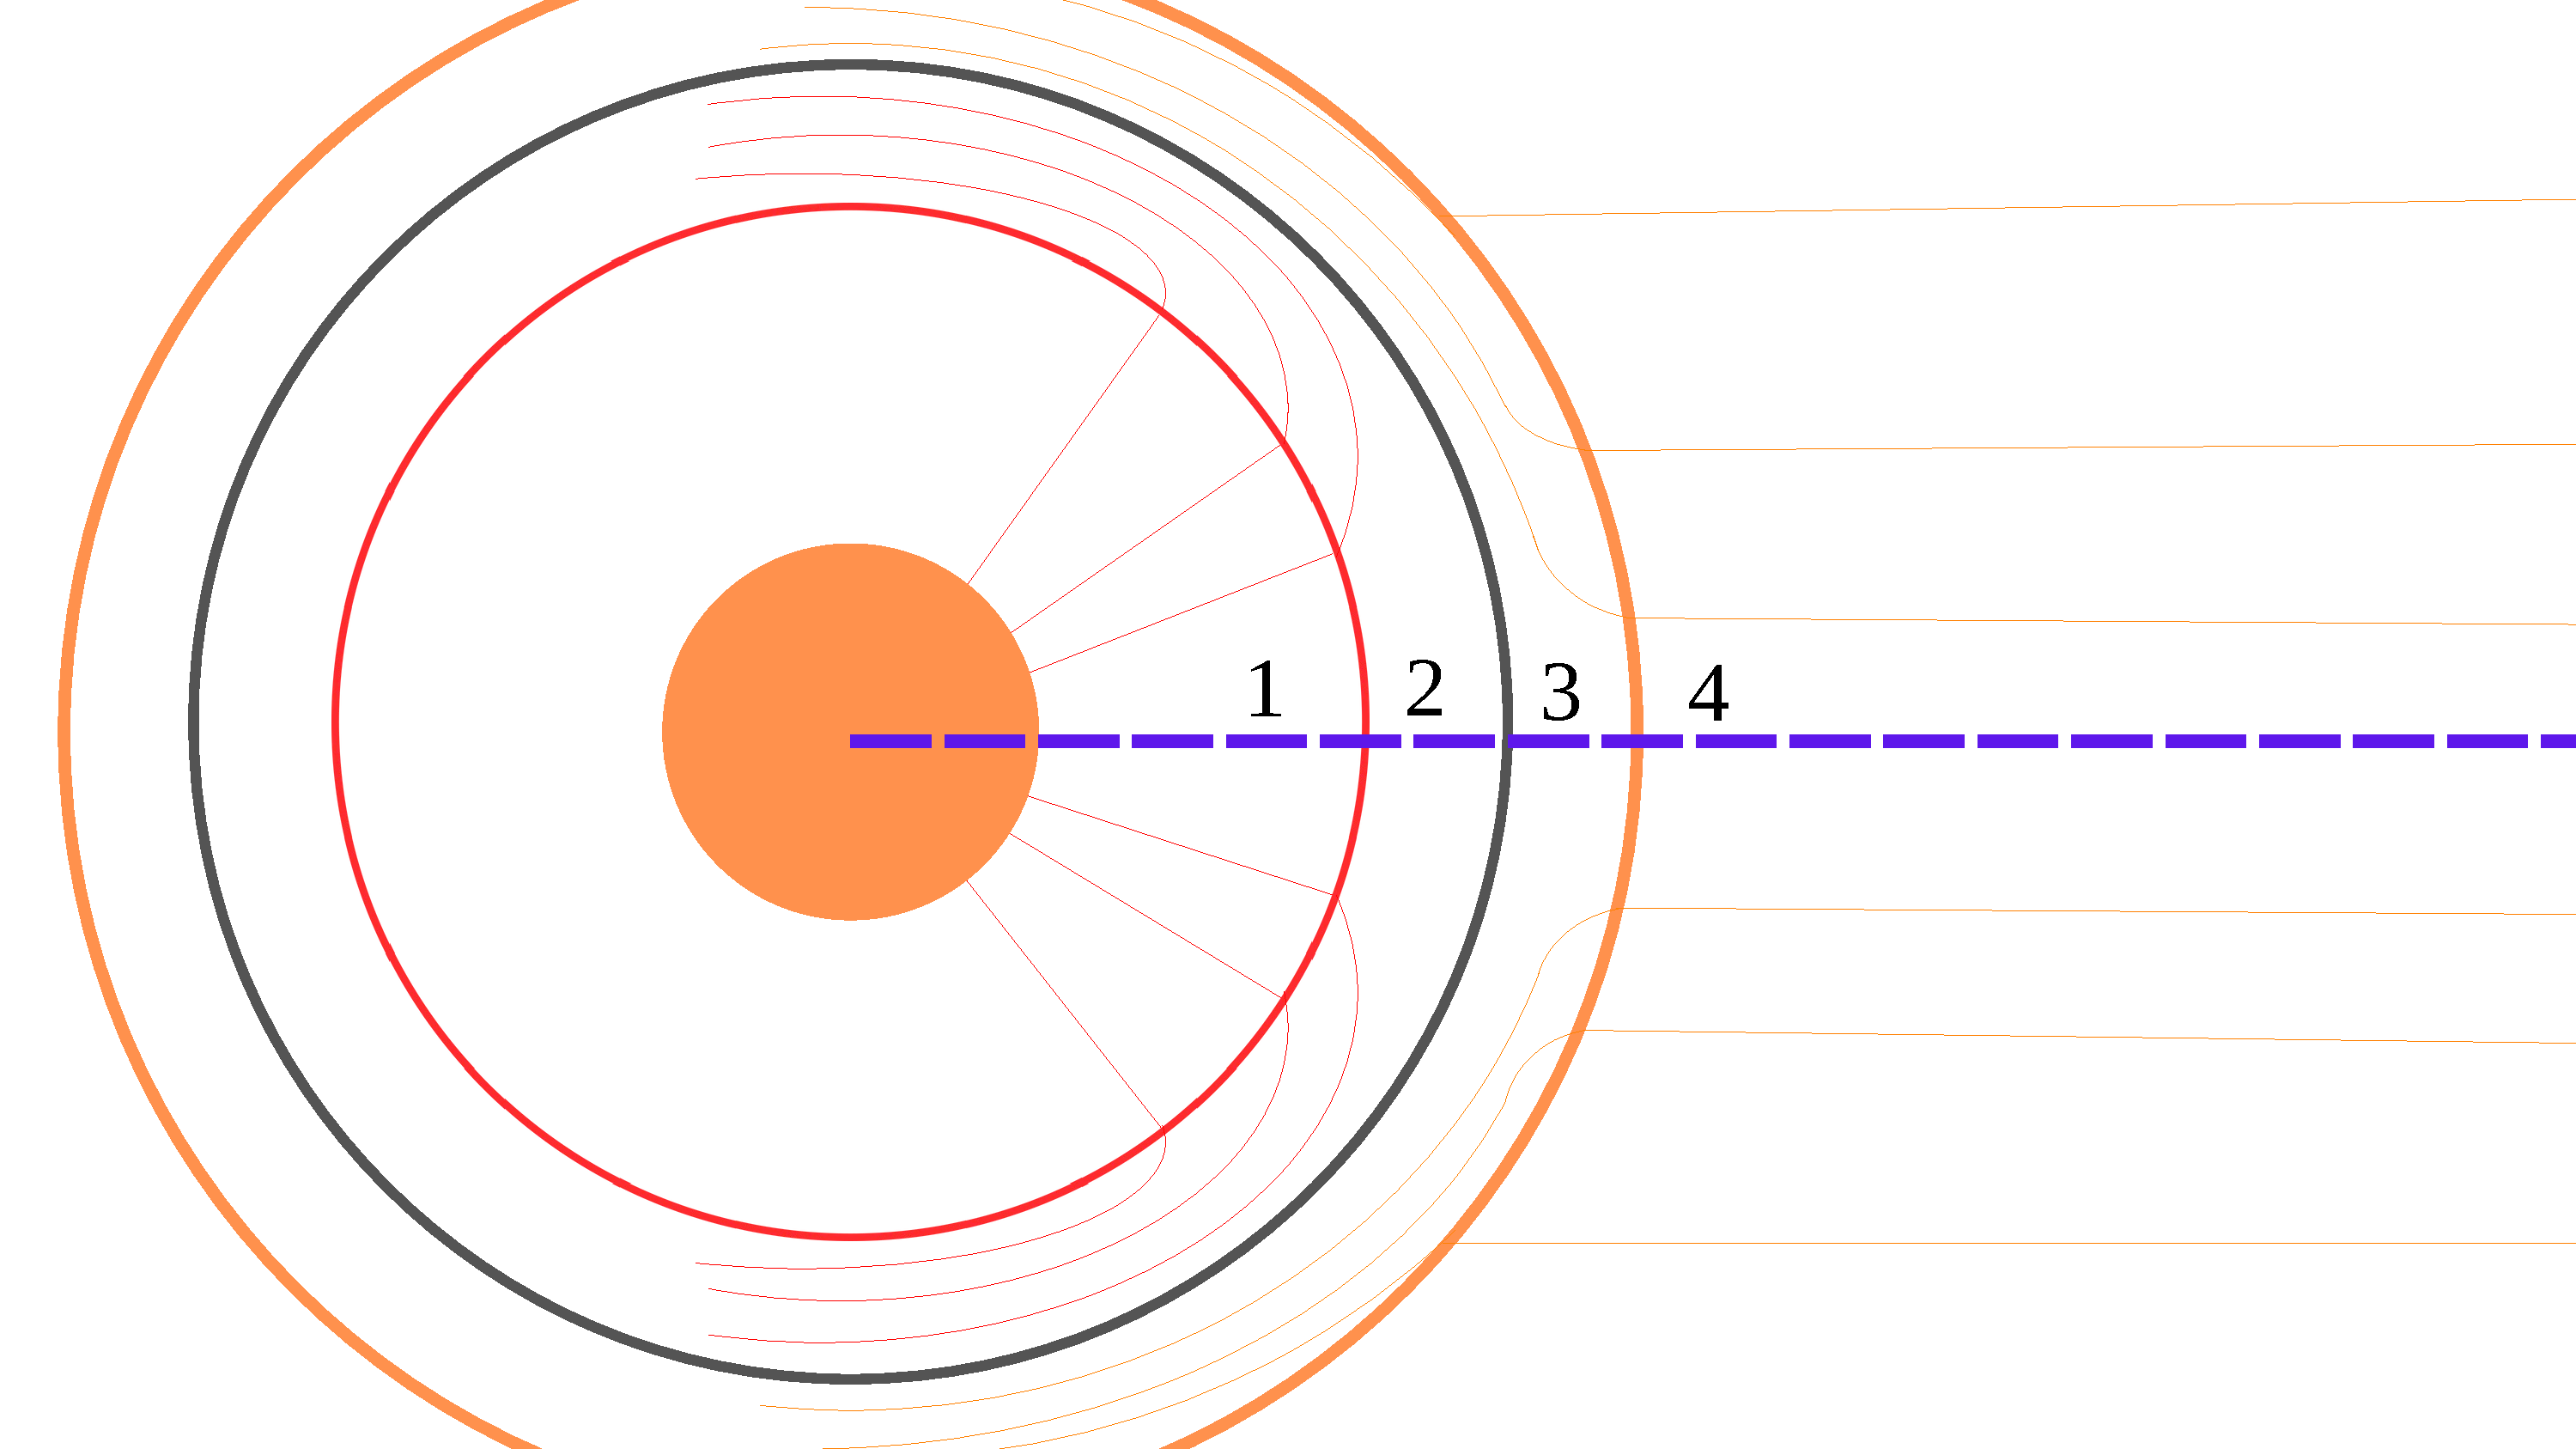
\includegraphics[width=\textwidth]{artesanales/ImgFi01-1.pdf}
    \caption{La interacción entre el flujo fotoevaporativo y el viento estelar de una estrella forma 4 zonas. La línea punteada que une al glóbulo con la estrella es el eje de simetría que vamos a considerar, vemos como en esta línea tanto el viento estelar como la radicación inciden de forma perpendicular a la base del glóbulo y en dirección contraria viaja el flujo fotoevaporativo. La zona 1 es donde el flujo fotoevaporativo sale de la superficie del glóbulo con un número de Mach igual a 1 y va aumentando, la zona 2 es el flujo fotoevaporativo chocado, la cual esperamos ver en las observaciones como una cáscara, la zona 3 es el viento chocado y la zona 4 es donde viaja el viento estelar supersónico, el cual es menos denso que el flujo fotoevaporativo. La discontinuidad de contacto se da entre las zonas 2 y 3}
    \label{fig:zones}
\end{figure}

A pesar de que la interacción entre el flujo fotoevaporativo y el viento estelar se da como en la figura \ref{fig:cilindross}, podemos simplificar este problema si suponemos que el nudo es esférico y solo nos fijamos en el eje de simetría que se puede apreciar en la misma imagen. La ventaja de usar este eje de simetría es que alrededor de este podemos considerar un cilindro de radio pequeño y considerar una simetría cilíndrica. Dentro de este cilindro podemos ignorar los movimientos transversales y así tratarlo mejor como un problema radial sobre este eje de simetría. En este eje de simetría tenemos la ventaja de que tanto el viento estelar como el flujo radiativo viajan de manera perpendicularmente a la superficie del nudo y el flujo fotoevaporativo viaja en dirección de estos. 

\begin{figure}[h]
    \centering    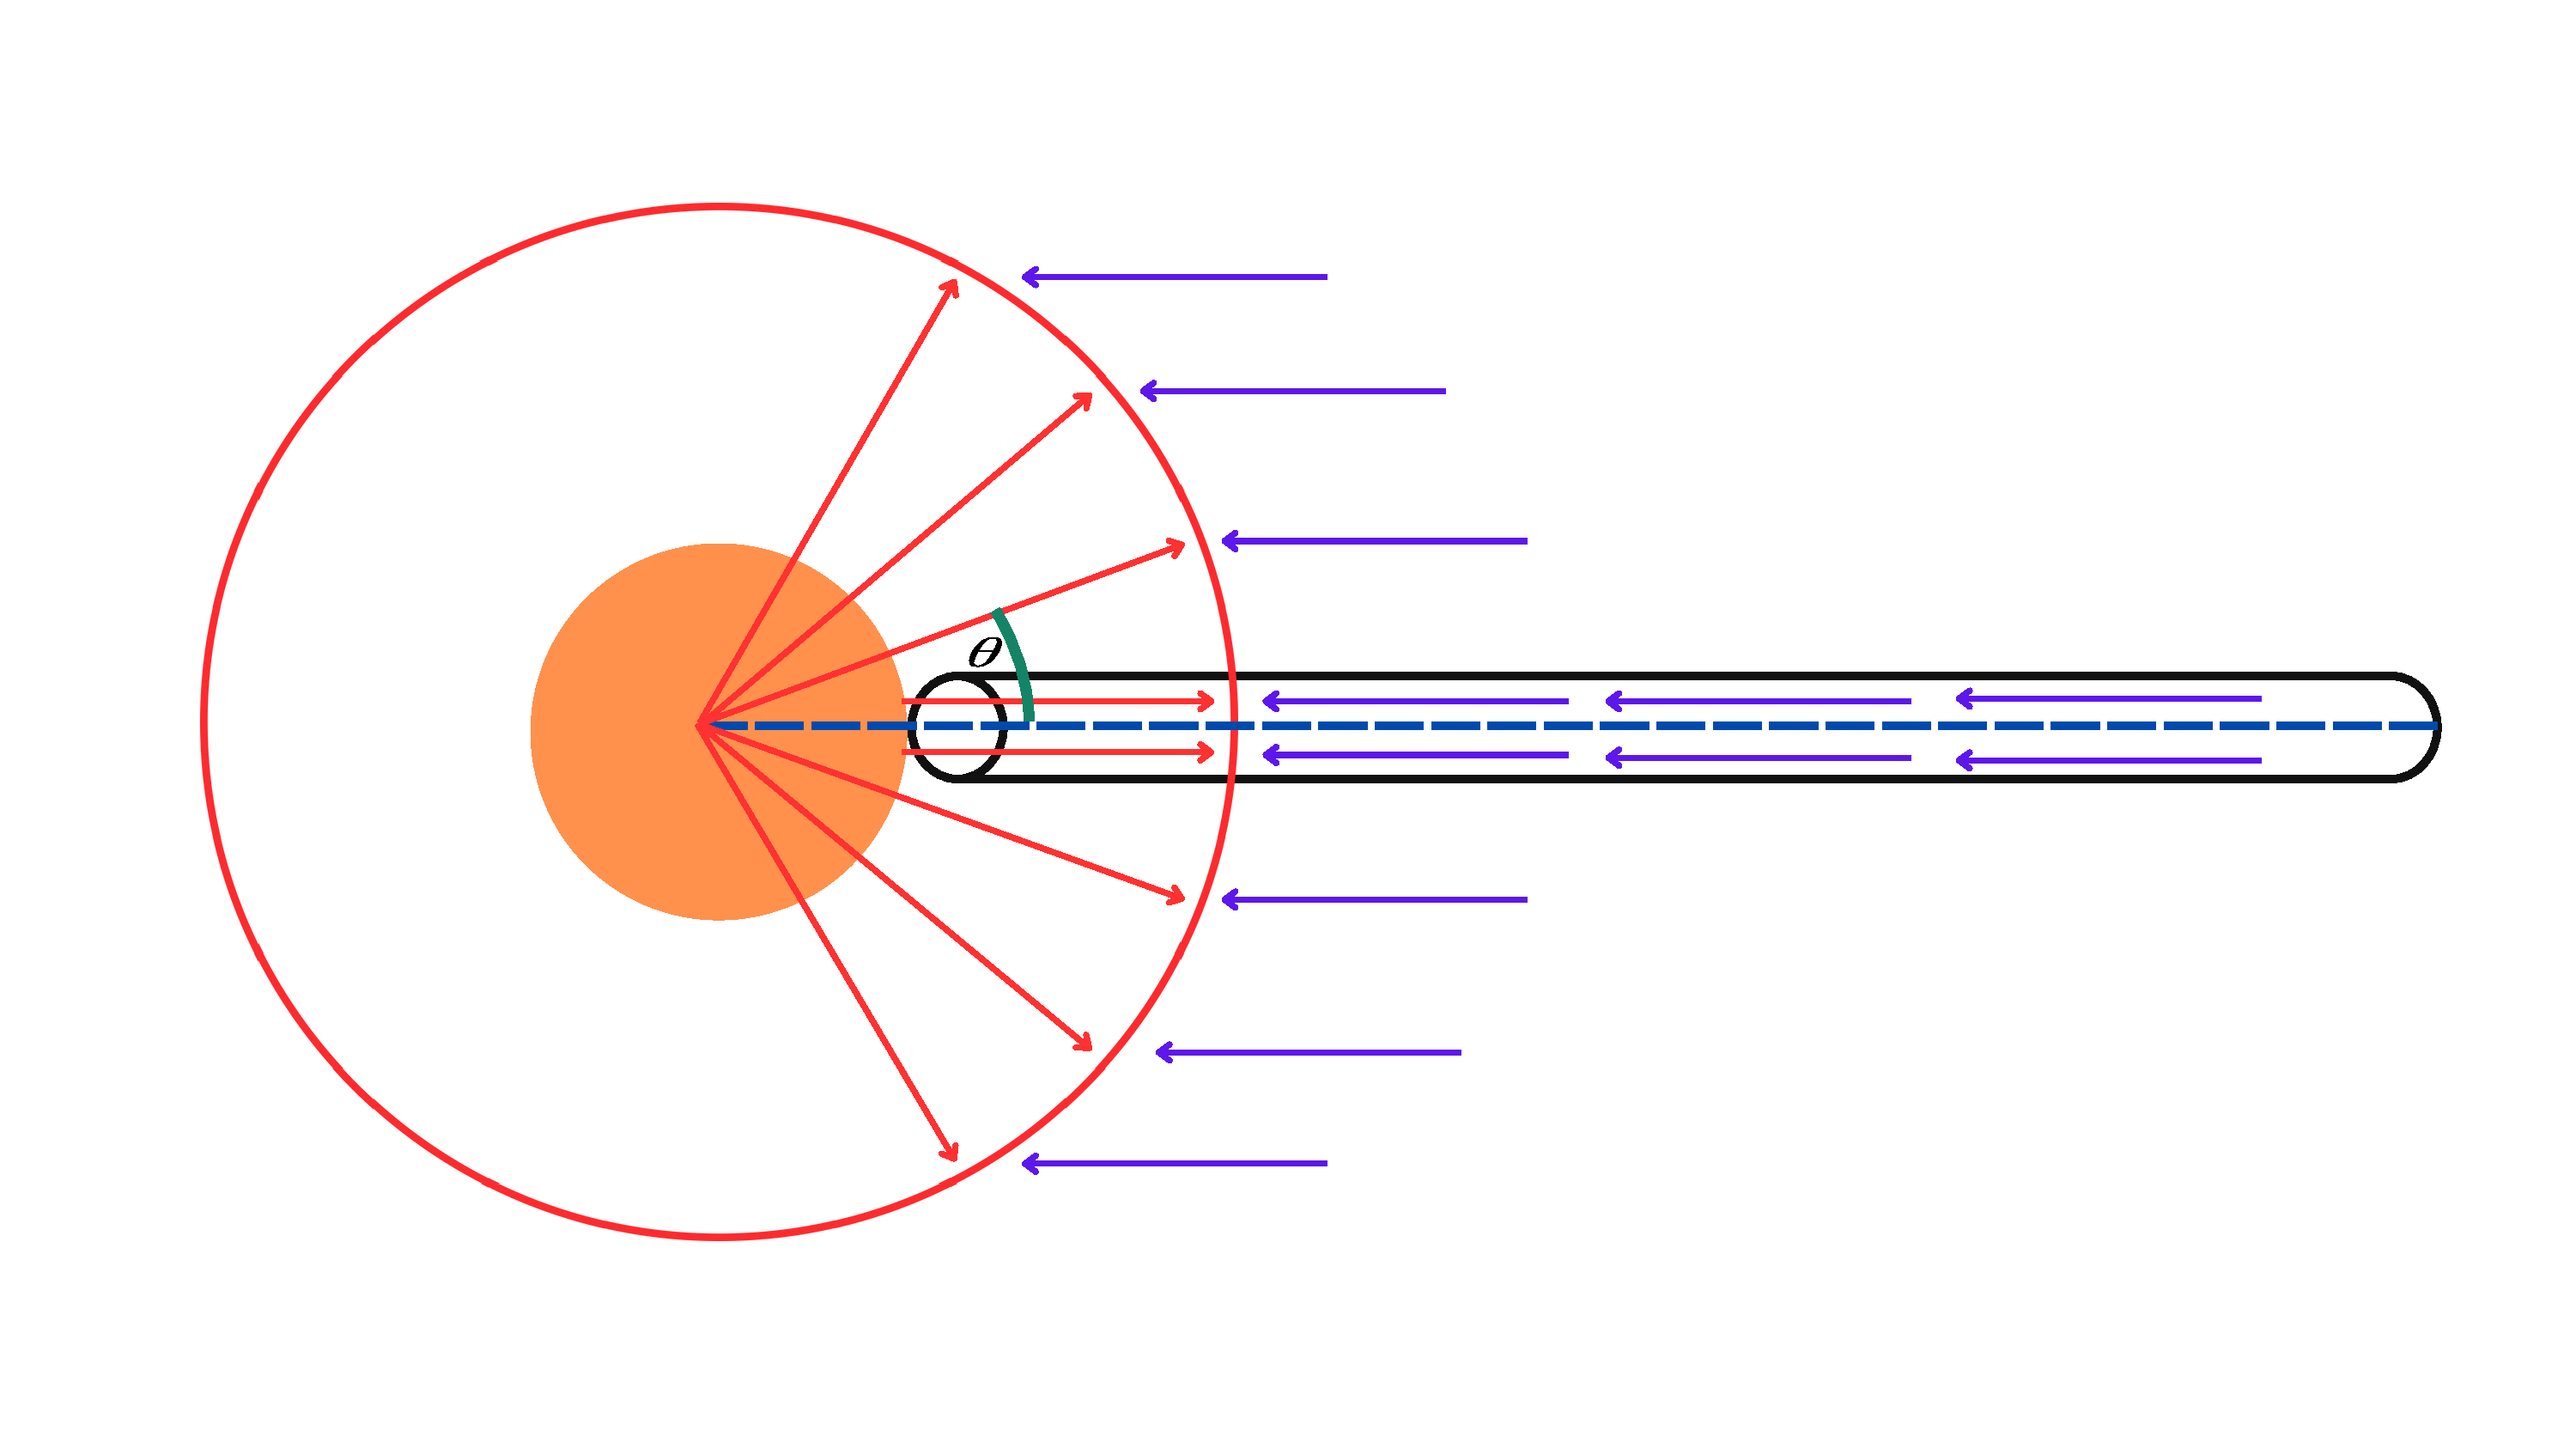
\includegraphics[width=\textwidth]{artesanales/ImgFi01-2.pdf}
    \caption{La radiación y el viento estelar viajan hacia el glóbulo como lo indican las flechas azules y vemos que inciden de manera perpendicular a la superficie del glóbulo en el eje de simetría. Mientras que el flujo fotoevaporativo por parte del glóbulo viaja como lo indican las flechas rojas, y por lo tanto en la interacción entre este flujo fotoevaporativo y el viento estelar debemos considerar cierto ángulo si no estamos en el eje de simetría.}
    \label{fig:cilindross}
\end{figure}

%\begin{figure}[h]
%    \centering    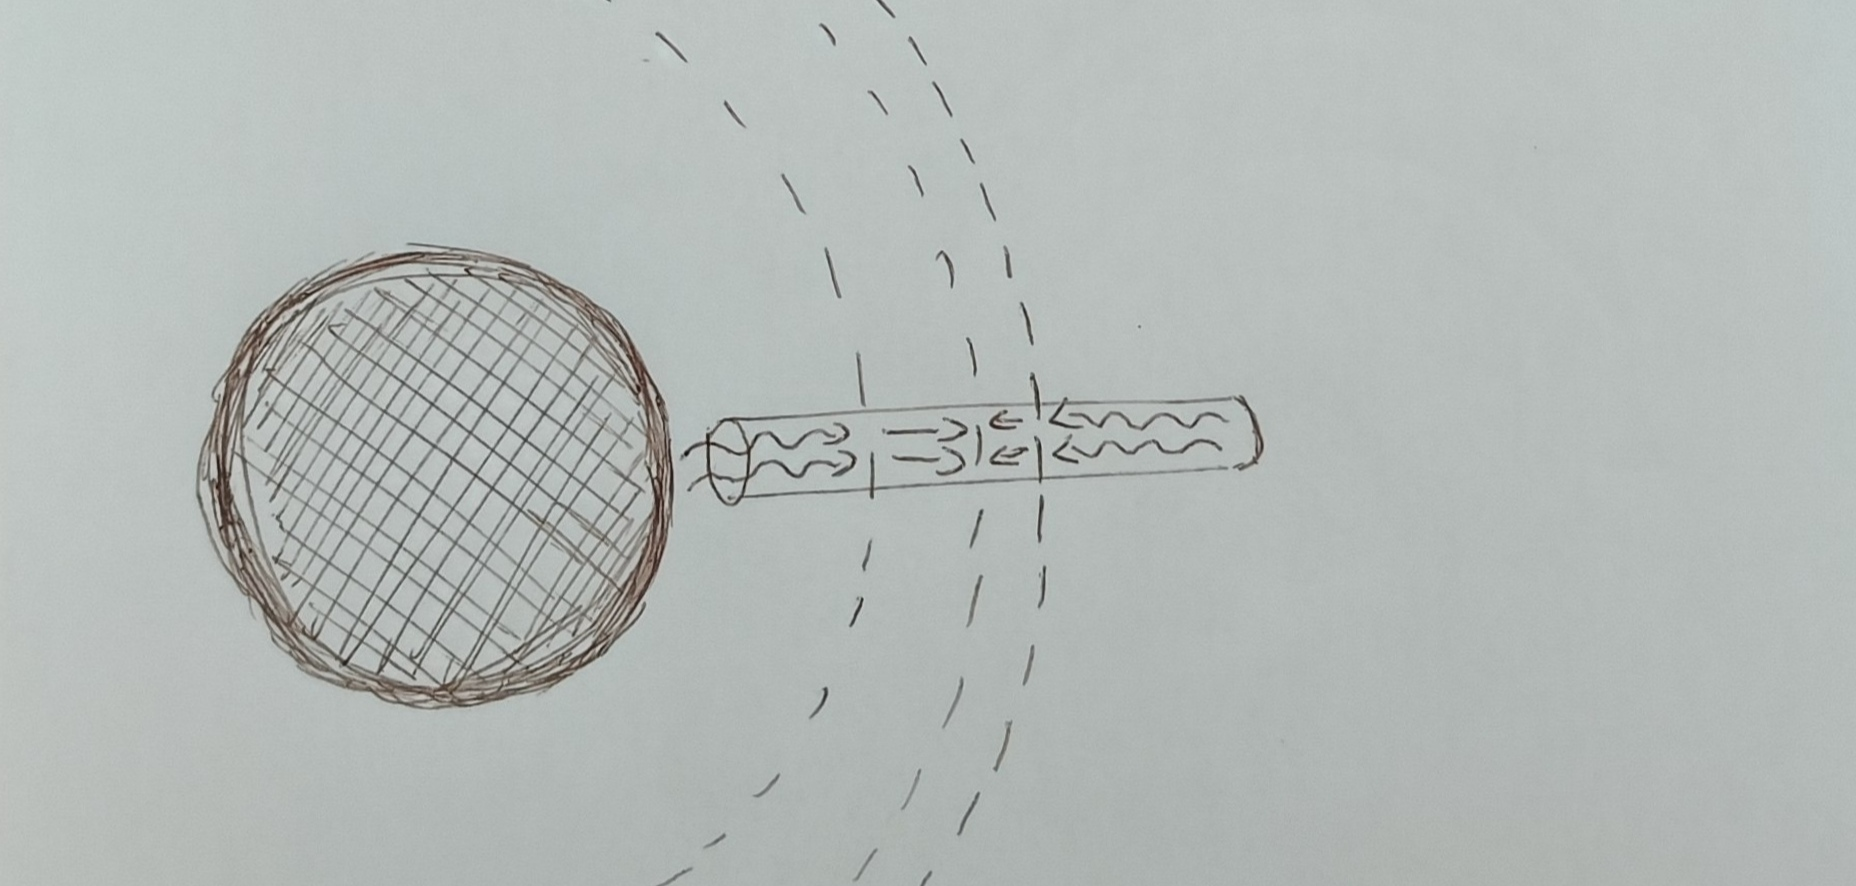
\includegraphics[width=0.75\textwidth]{images Chapter 2/Chp2_cilinders.jpg}
 %   \caption{Si consideramos una simetría cilíndrica con un radio muy pequeño, podemos tratar este problema de manera radial y de tal manera que la radiación y el viento estelar inciden de manera perpendicular al glóbulo.}
 %   \label{fig:cilinders}
%\end{figure}

\section{Modelo hidrodinámico estacionario}

Para este modelo es importante mencionar que no estamos considerando ninguna fuerza de gravedad por parte de la estrella o del mismo glóbulo\footnote{Esta y otras simplificaciones se justifican en los Apéndices.}, así como tampoco vamos a considerar campos magnéticos por simplicidad.

Tomando en cuenta que el tiempo en el que ocurren las fases mencionadas en la sección \ref{Sec:fluijos fotoevaporativos} es muy corto comparado con el tiempo de interacción que hay entre el flujo fotoevaporativo y el viento estelar, vamos a suponer que la capa aislante producida por la radicación UV ya se ha formado y ahora estamos en equilibrio de ionización. Por lo que vamos a considerar este modelo como estacionario. 

Como ya se mencionó antes, podemos tener una simetría cilíndrica alrededor del eje de simetría que une al nudo con la estrella. De esta manera podemos ignorar los movimientos transversales ya que los gradientes en estas direcciones son muy pequeñas si los comparamos con los gradientes en la dirección axial.

Como vemos en la figura \ref{fig:cilindross} en el eje de simetría el viento estelar incide en sentido contrario al flujo fotoevaorativo y de manera perpendicular a la superficie del nudo, por lo que aquí el problema se vuelve unidimensional y es más fácil de resolver. Fuera del eje de simetría el flujo fotoevaporativo sigue viajando de manera radial pero con cierto ángulo con respecto al eje de simetría como vemos en la figura \ref{fig:cilindross}, además tanto la radiación fotoionizante como el viento estelar ya no inciden de manera perpendicular a la superficie del nudo, por lo que deberíamos tomar en cuenta el ángulo en que se encuentra. Es por esta razón que en principio vamos a resolver este problema de manera unidimensional en el eje de simetría.

% Balance between ionizations and recombinations

\section{Ecuación de estado y equilibrio de ionización}

Para este caso vamos a considerar que el gas que esta interaccionando con la radicación de la estrella es un gas ideal, por lo que nuestra ecuación de estado será
\[PV = Nk_BT\] donde $P$ tiene unidades de presión, $V$ unidades de volumen, $N$ es el número de partículas, $k_B$ la constante de Boltzman con unidades de \SI{}{erg.K^{-1}} y $T$ es la temperatura con unidades de \SI{}{K}. De aquí tenemos que \[P = nk_BT = \frac{\rho k_B T}{\bar{m}}\] donde $n$ es la densidad numérica, $\rho$ la densidad de masa y $\bar{m}$ es la masa promedio. En este caso estamos considerando que el gas contiene principalmente hidrógeno y una pequeña fracción de helio, por lo que vamos a considerar una masa promedio de \SI{0.6}{m_{p}} en el gas ionizado.

En este gas ideal vamos a tomar la velocidad del sonido isotérmica, la cual está dada por
\[c_s  = \sqrt{\frac{k_B T}{\bar{m}}}\] de esta manera vemos que la velocidad del sonido en el gas ionizado solo depende de su temperatura. En este tipo de gases la velocidad del sonido es típicamente del orden de \SI{e6}{cm.s^{-1}}

En este modelo vamos a considerar que  ya ha sucedido la tormenta de partículas ionizantes, la fase de implosión y se ha formado la capa aislante como se mencionó en la sección \ref{Sec:fluijos fotoevaporativos}, por lo que vamos a considerar que el flujo de fotones ionizantes por unidad de tiempo por parte de la estrella ionizante 
\[S_* = \int_{\nu_0}^\infty \frac{L_\nu}{h\nu}d\nu\] donde $L_\nu$ es la luminosidad de la estrella por unidad de frecuencia y $\nu_0$ es la frecuencia a la que los fotones tienen energía de \SI{13.6}{eV}, esta en equilibrio con la tasa total de recombinaciones que esta dada por 
\[\dot{n}_{rec}=n_e n_i h \alpha_\mathrm{B}+n_0u_0\] donde $\alpha_\mathrm{B}$ es el coeficiente de recombinación para el caso B. Este coeficiente de recombinación para el caso B toma en cuenta las recombinaciones a todos los niveles, excepto al nivel base, esto ya que el fotón liberado en esta recombinación al nivel base puede volver a ionizar algún otro átomo que se encuentre muy cerca. El segundo término se refiere a las partículas que cruzan el frente de ionización ya que, como ya habíamos mencionado antes, el frente de ionización avanza en dirección al glóbulo por lo que debemos considerar las nuevas partículas que deben ionizarse. 

\section{Estructura del modelo}\label{Estructura}

En este modelo  estamos considerando un frente D-crítico para el frente de ionización \citep{Shuu:1992}, esto es, que en la parte neutra tenemos una expansión subsónica y hay un punto sónico interios al frente de ionización a partir del cual tendremos una expansión supersónica en la zona ionizada. En este caso por simplicidad vamos a considerar el frente de ionización como una discontinuidad en el que pasamos de tener gas no ionizado a tener un gas totalmente ionizado por lo que tomaremos que el punto sónico se da en $r_0$. Así que vamos a considerar que el gas tiene un número de Mach igual a 1 en $r_0$ y este va a ir aumentando conforme atraviesa toda la zona 1 de la figura \ref{fig:zones} ya que se va expandiendo libremente. En principio podríamos tomar que tanto el radio del glóbulo como la densidad en su superficie son parámetros libres, pero con las observaciones podemos medir el radio y la densidad la podemos calcular ya que esta debe ser consistente por haber considerado equilibrio de ionización.

Con este modelo se pretende ver hasta donde llegamos a un equilibrio de presión entre la presión por parte del flujo fotoevaporativo y la presión RAM del viento estelar. Para el caso de la presión del flujo fotoevaorativo vamos a considerar tanto la presión térmica como la hidrodinámica por lo que la presión total está dada por
\[P_{tot}=P_{ter}+P_{hid}=n\bar{m}c_s^2+n\bar{m}u^2=\rho c_s^2(1+M^2)\]
En este caso no estamos considerando presión magnética ni de radiación.

\begin{figure}[h]
    \centering 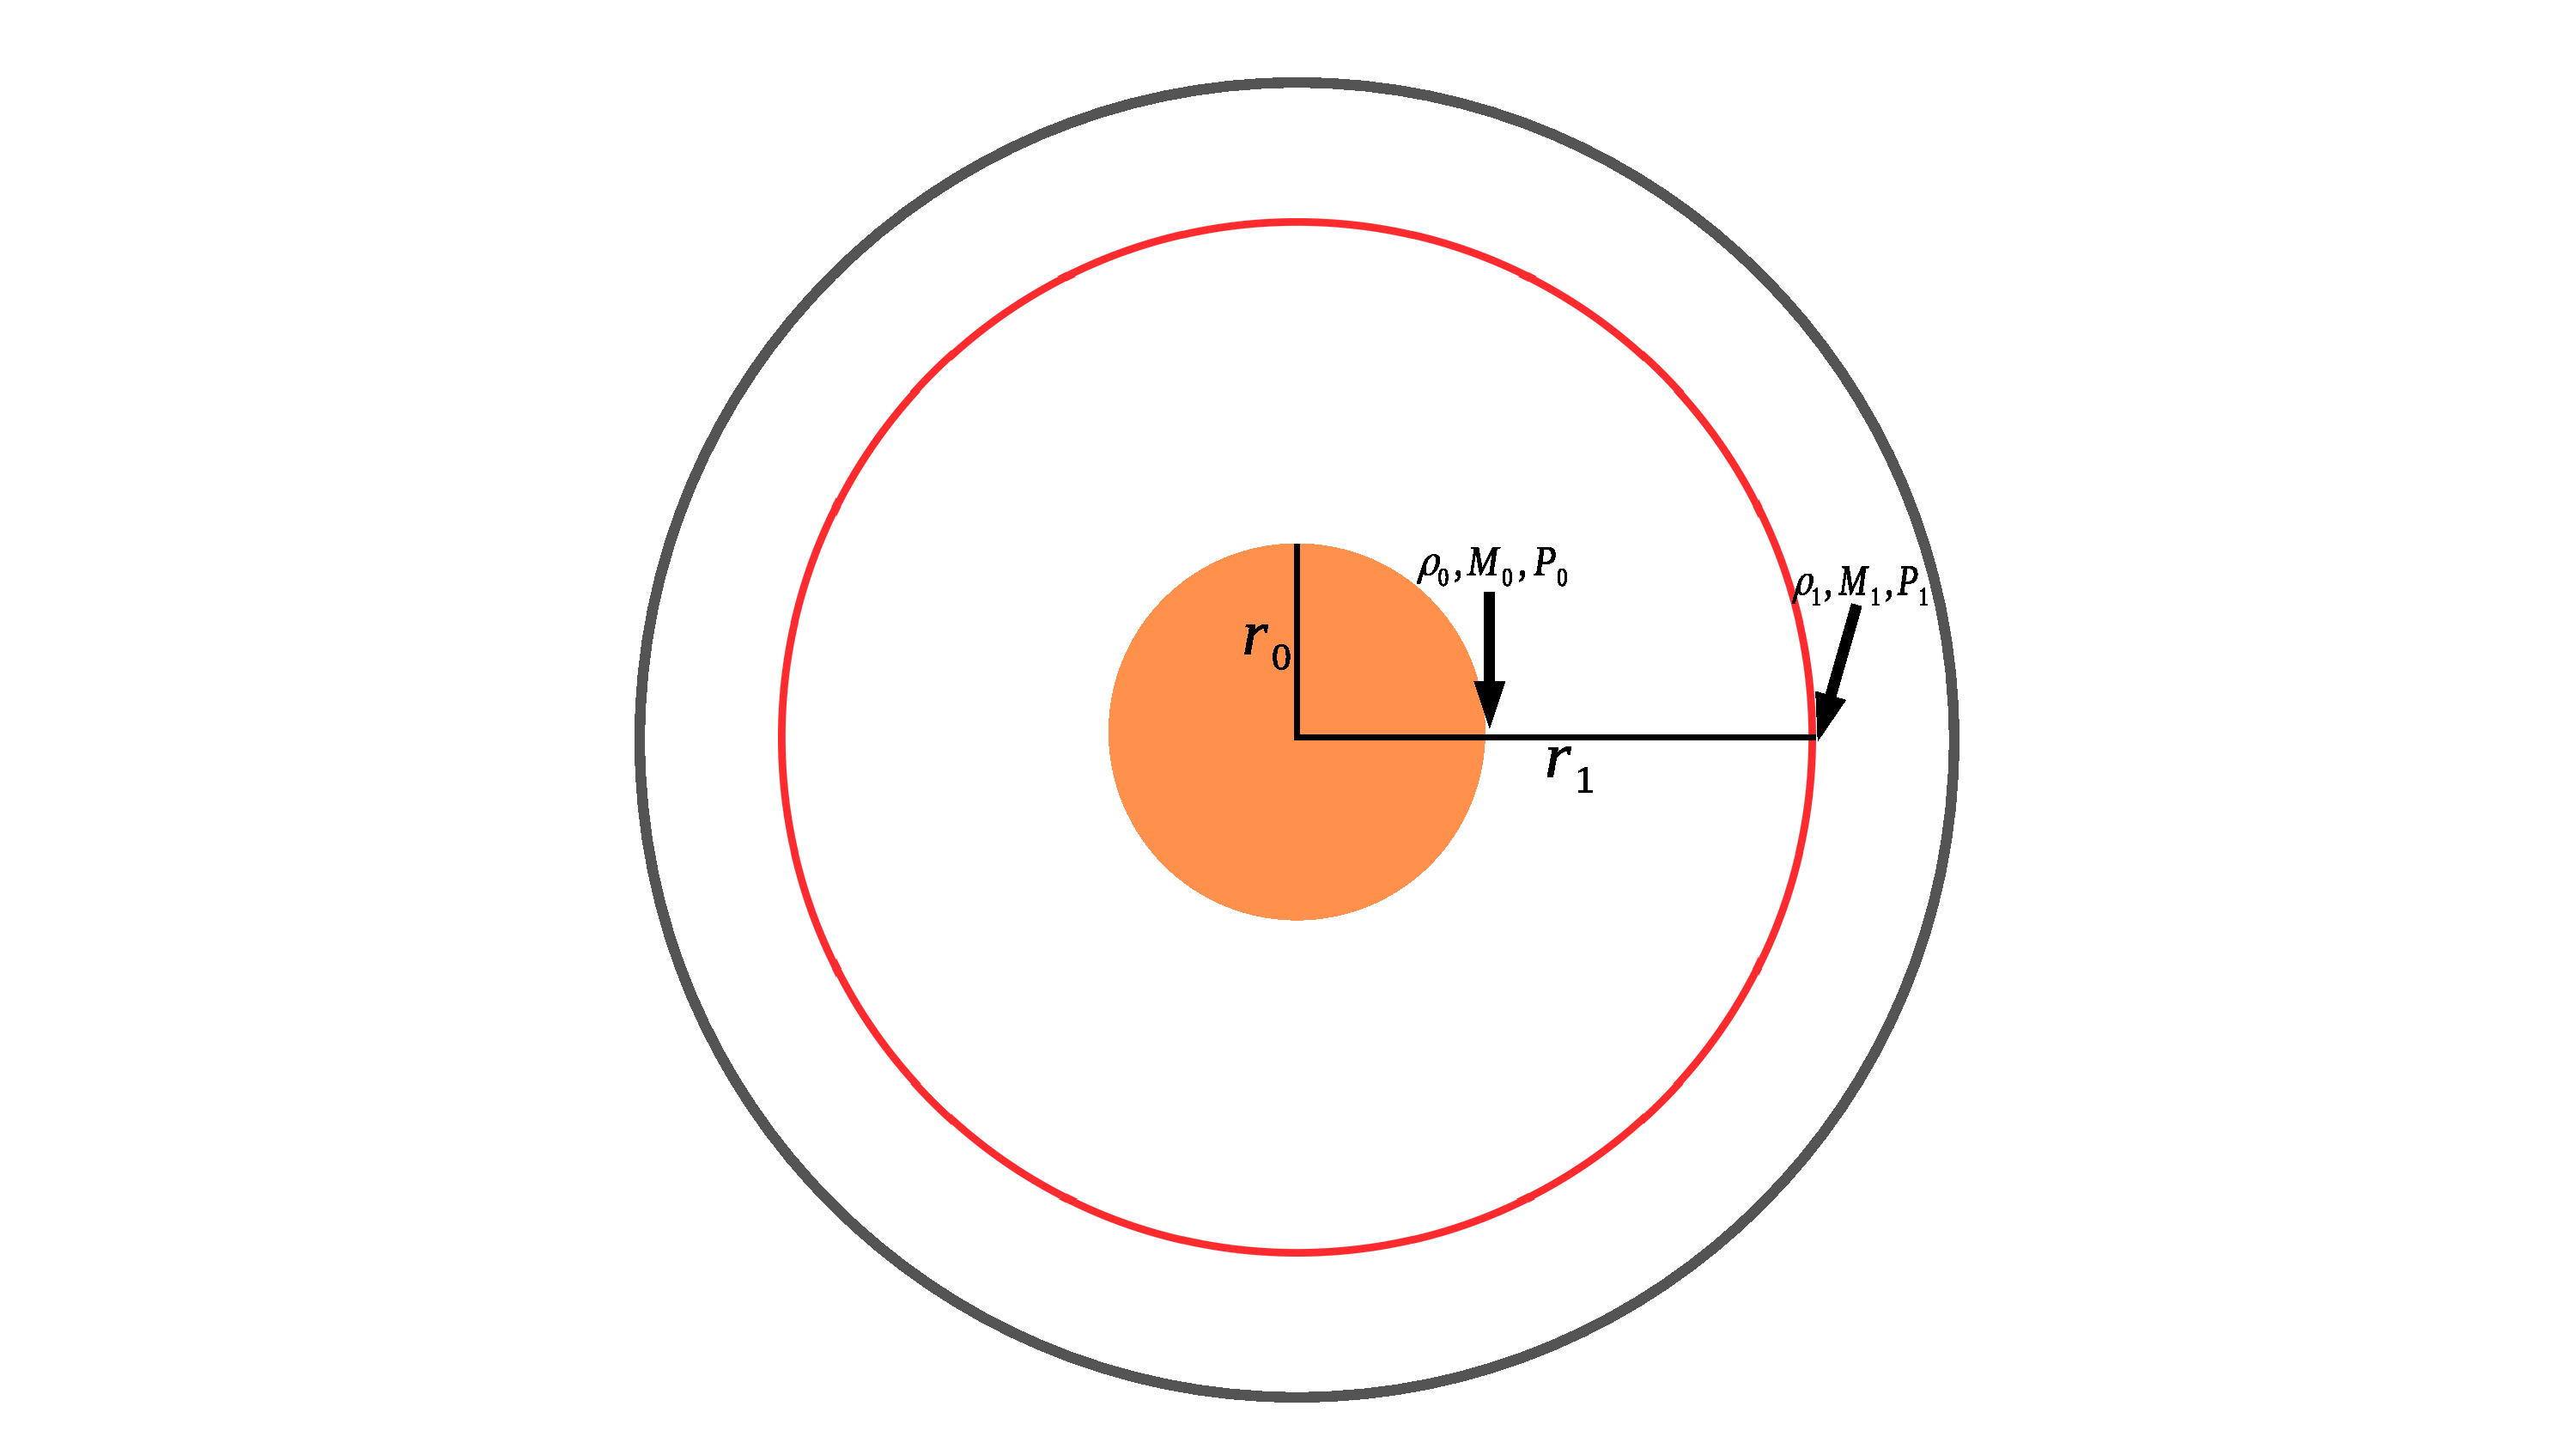
\includegraphics[width=\textwidth]{artesanales/ImgFi01-3.pdf}
    \caption{$r_0$ es el radio del glóbulo, la parte neutra, mientras que $\rho_0,M_0$ y $P_0$ son los valores que tenemos en la superficie del glóbulo y conforme estos avanzan con dirección a la estrella sus valores van cambiando hasta tener diferentes valores en $r_1$, que el radio del centro del glóbulo hasta la base del flujo fotoevaporativo chocado, $\rho_1,M_1$ y $P_1$ son los valores que tendrán en la base del flujo fotoevaporativo chocado.}
    \label{fig:parameters}
\end{figure}

Este equilibrio de presión se logrará a un radio $r_1$ que es donde la presión del flujo fotoevaporativo ha disminuido un fracción $f$ de lo que era la presión inicial. Por lo que la presión cambia como 
\[f=\frac{P}{P_0}=\frac{\rho c_s^2(1+M^2)}{\rho_0 c_s^2(1+1)}=\frac{\rho}{\rho_0}\frac{1+M^2}{2}\]
Considerando la ecuación para la conservación de masa tenemos que
\[\rho r^2M	=\rho_0 r_0^2\]
y finalmente si consideramos la ecuación de Bernoulli isotérmica 
\[\frac{v^2}{2}+c_s^2\ln\rho=constante\]
tenemos que 
\[\frac{r}{r_0}=M^{-1/2}e^{\frac{M^2-1}{4}}\] \cite{Dyson:1968}.
Ahora que tenemos tres ecuaciones y tres incógnitas podemos resolver, en nuestro caso lo hicimos de manera numérica. Al resolver estas ecuaciones para diferentes $f$ tenemos que tanto la presión como la densidad decaen con el radio, mientras que el número de Mach aumenta como vemos en la figura \ref{fig:grafica_C2}.

\begin{figure}[h]
    \centering    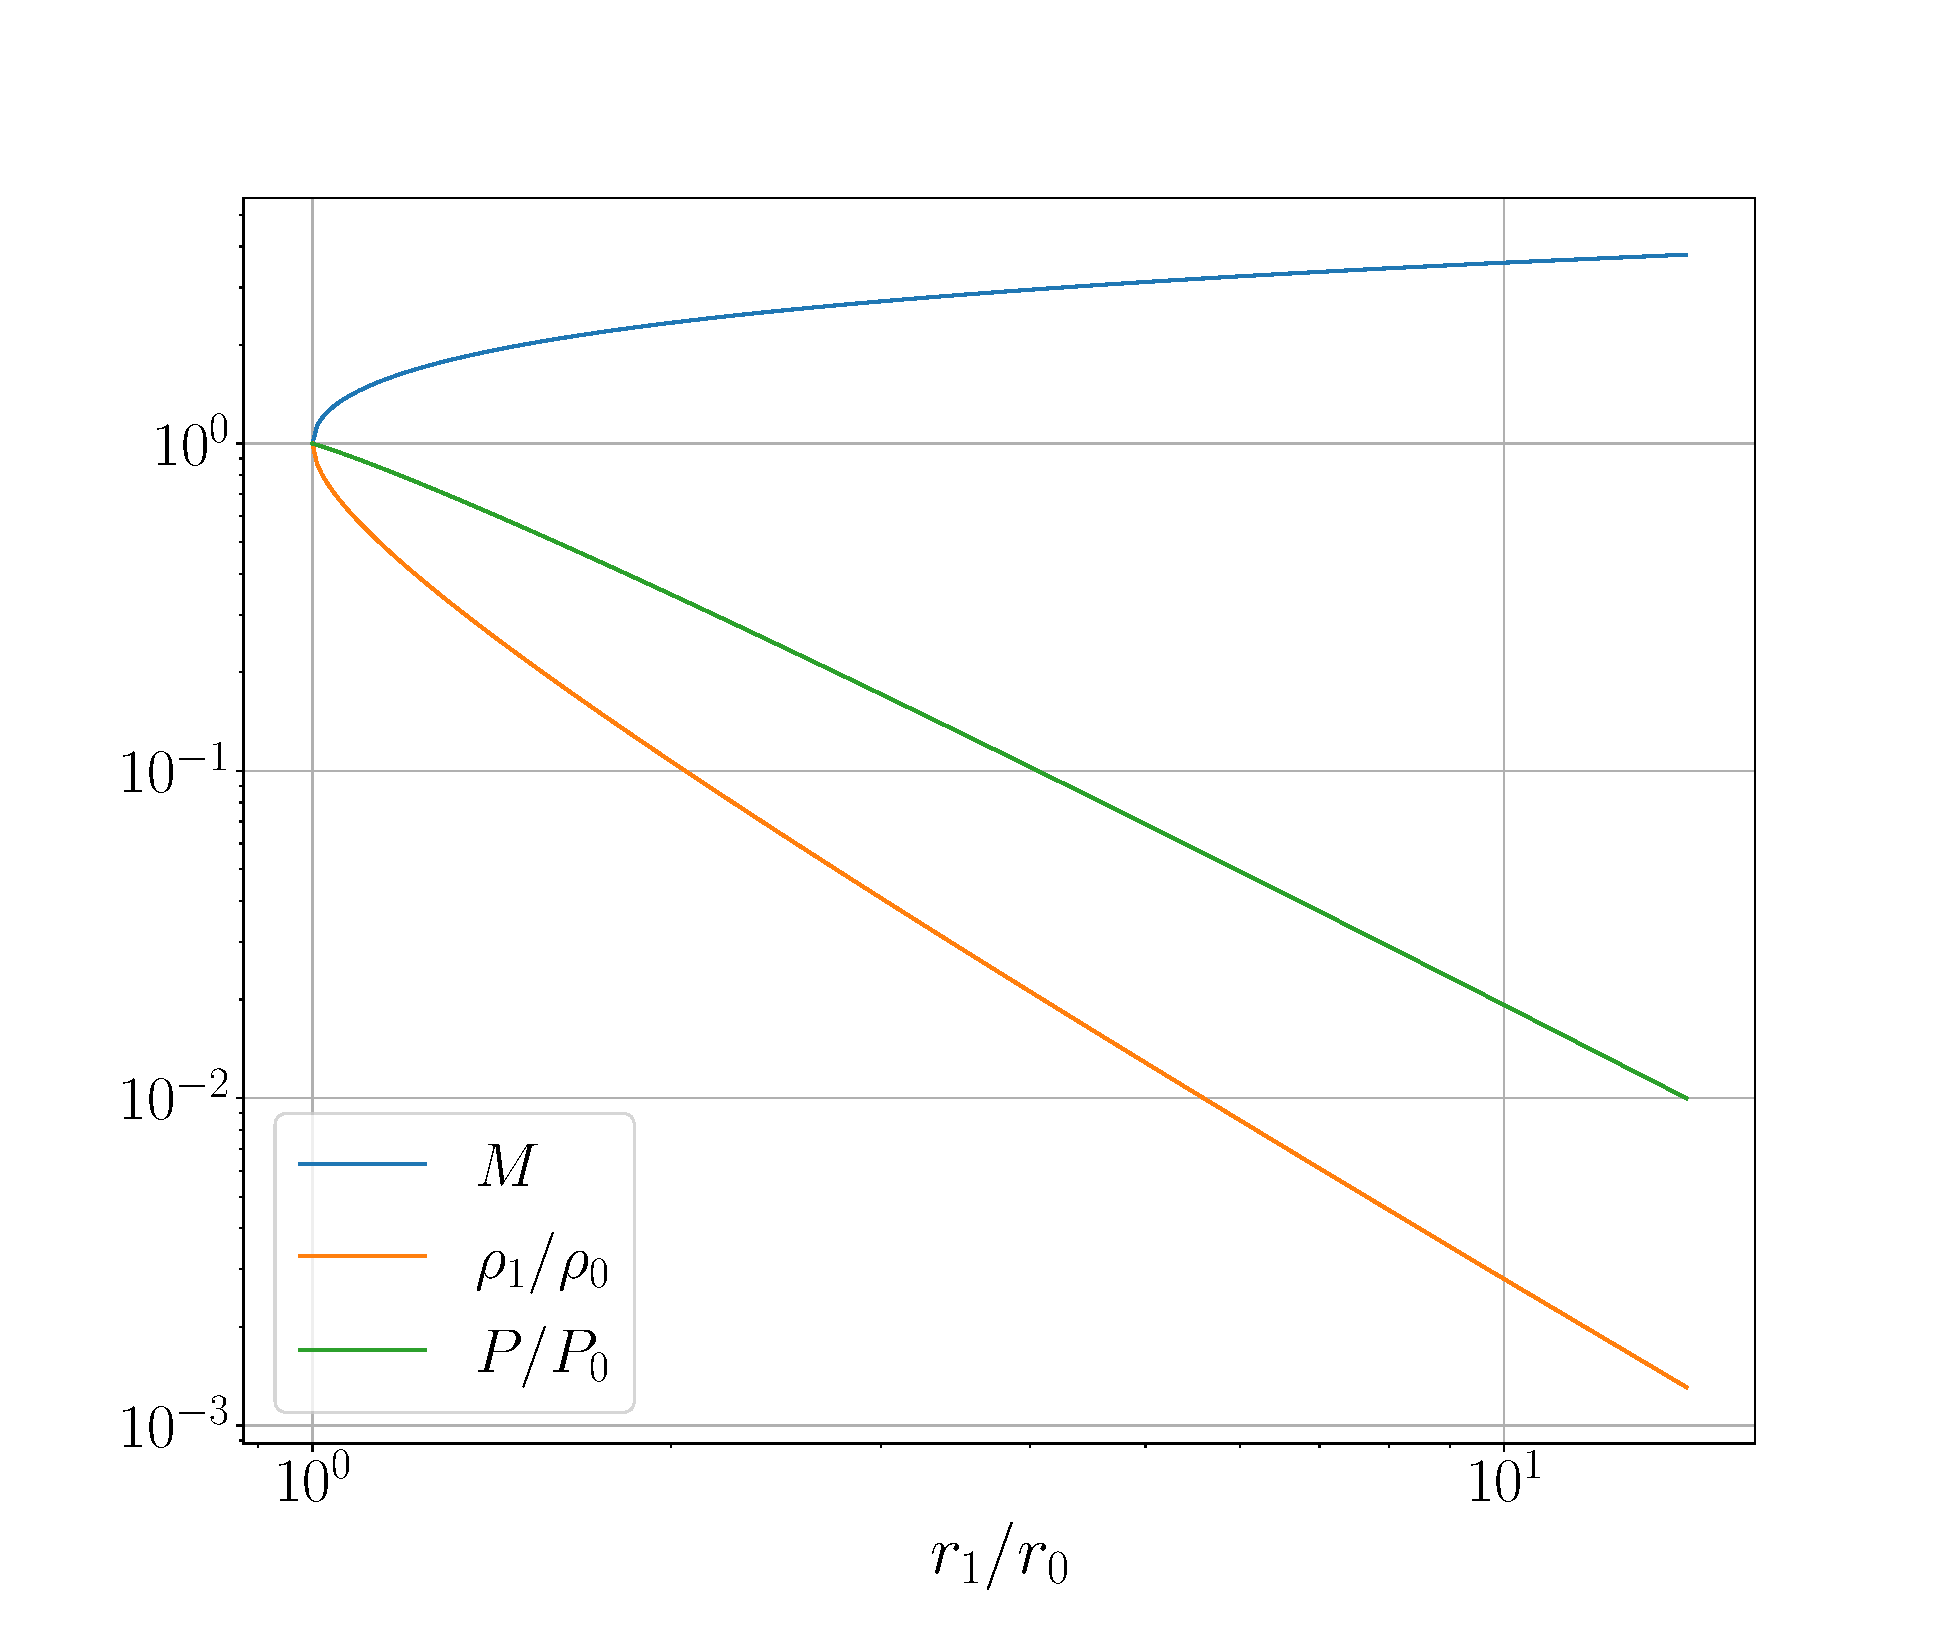
\includegraphics[width=0.8\textwidth]{images Chapter 2/Model.pdf}
    \caption{Gráfica de M, $\rho$ y $P$ normalizados como función de radio normalizado}
    \label{fig:grafica_C2}
\end{figure}

% Assumption of isothermal equation of state
\section{Condiciones para la cáscara chocada}

\cite{Canto:1996} trata de una manera formal la interacción entre dos flujos supersónicos en la cual considera dos fuentes separadas a una distancia D como en la figura \ref{fig:Canto1}. Cuando estos flujos que están interaccionando llegan a un equilibrio de presiones se forma una cáscara delgada, \cite{Canto:1996} da la solución a distintos parámetros $\beta$ el cual es la razón de los momentos de los flujos. Esto se puede ver en la figura \ref{fig:Canto2} en la cual notamos que cuando el momento de un flujo es muy  grande comparado con el otro la cáscara chocada se vuelve muy curva y está más cerca de la fuente cuyo flujo tiene menor momento.

\begin{figure}[h]
    \centering    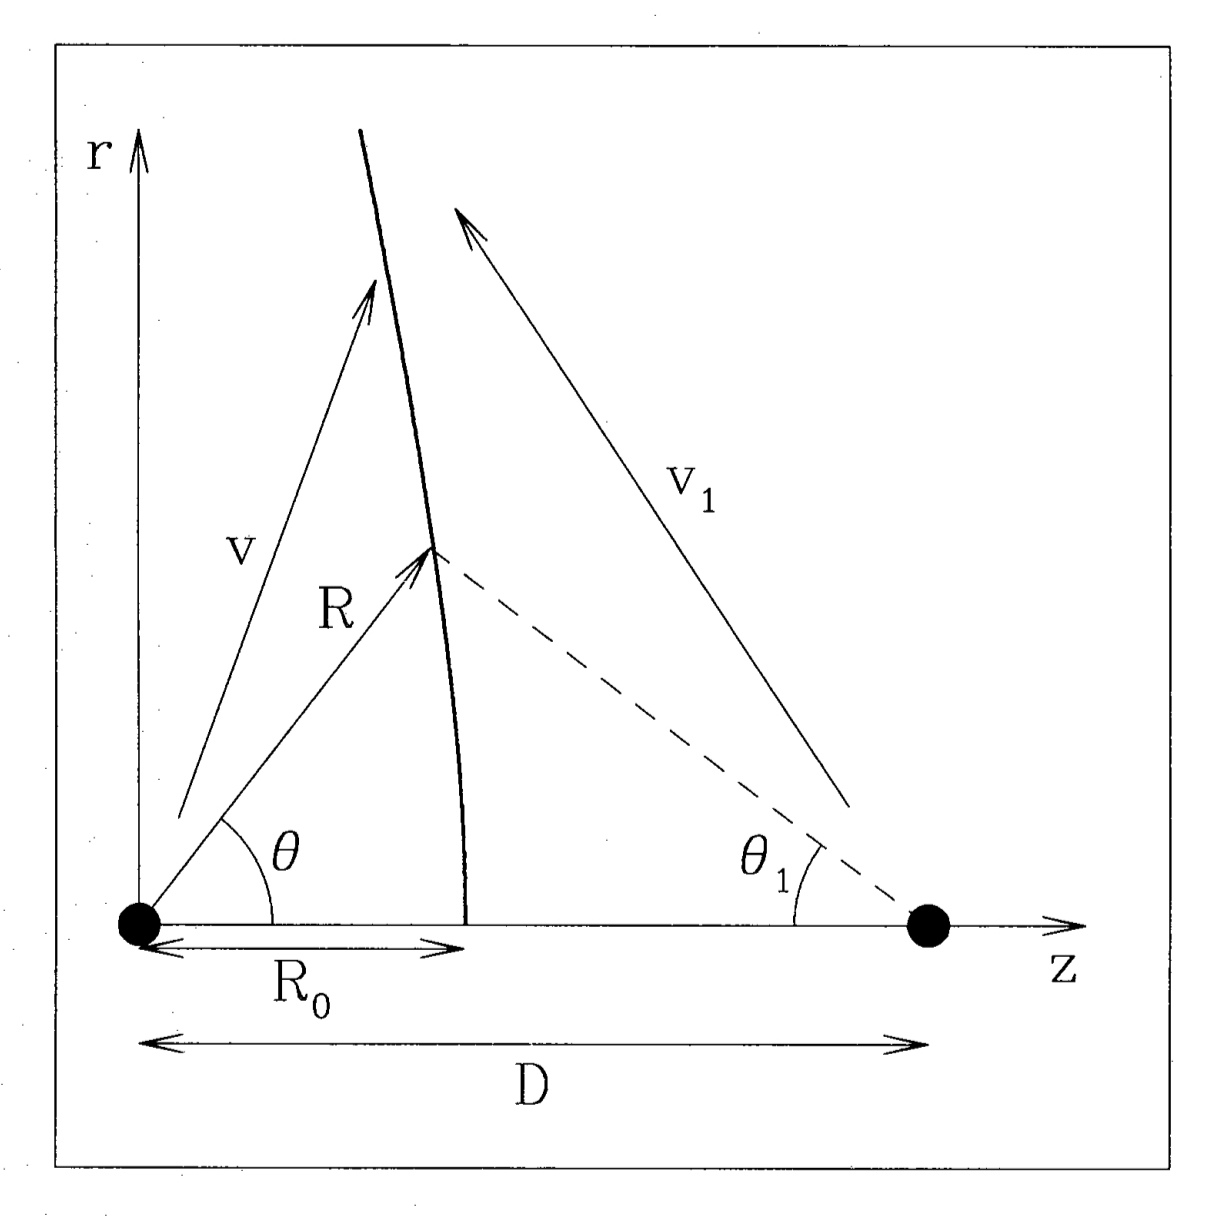
\includegraphics[width=0.8\textwidth]{images Chapter 2/C2_Canto.jpg}
    \caption{Interacción de dos flujos supersónicos las cuales son producidas por dos fuentes (puntos negro en el eje z) a una distancia D. En esta interacción se produce una cáscara delgada R$(\theta)$ cuando los flujos llegan a un equilibrio. Para este problema se considera simetría cilíndrica \citep{Canto:1996}.}
    \label{fig:Canto1}
\end{figure}

\begin{figure}[h]
    \centering    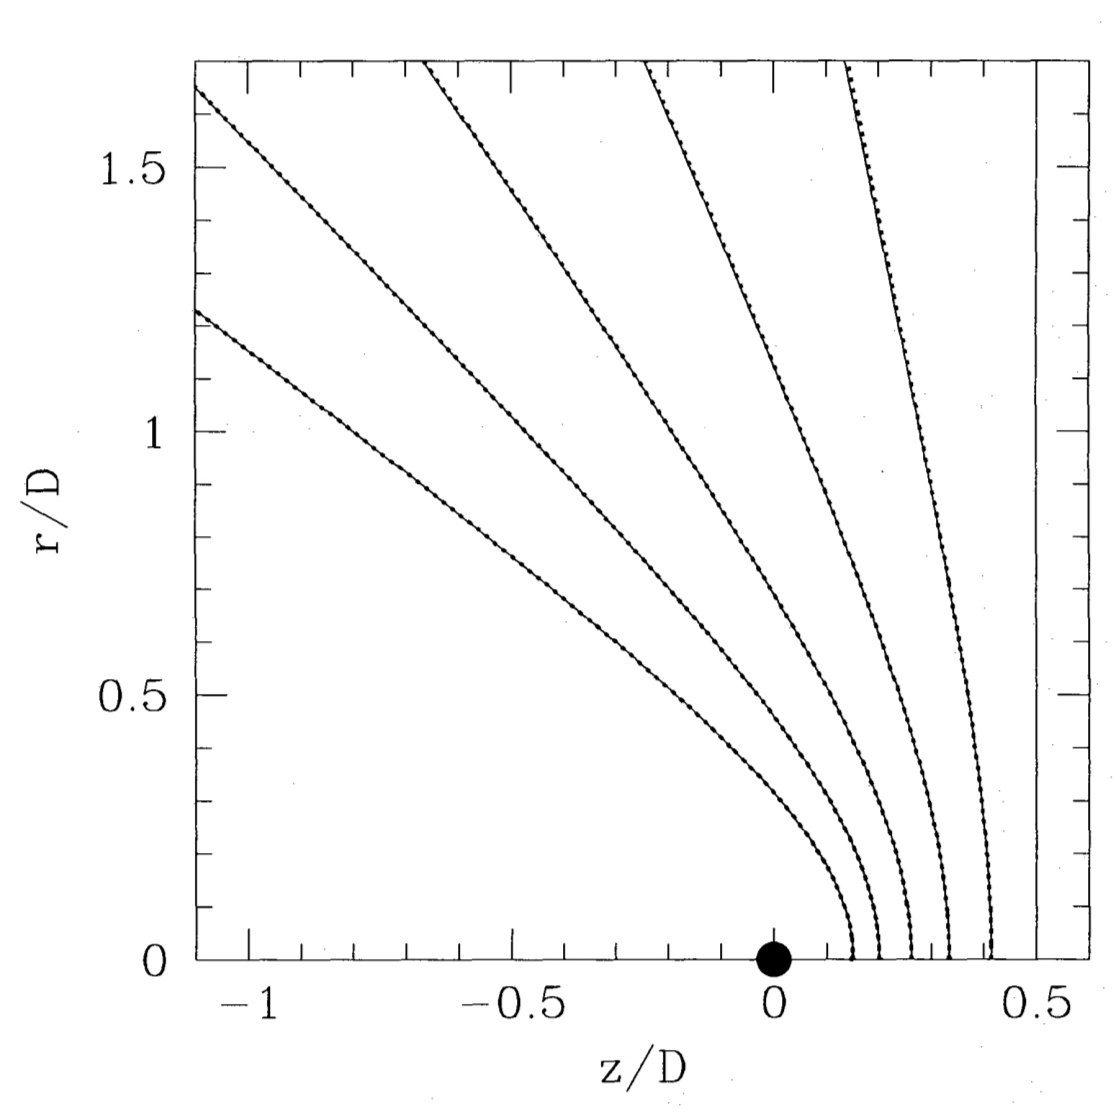
\includegraphics[width=0.8\textwidth]{images Chapter 2/C2_Canto2.jpg}
    \caption{Formas de las distintas cáscaras chocadas a diferentes parámetros $\beta$. La línea vertical en z/D=0.5 corresponde a un parámetro $\beta=1$ y las demás curvas corresponden a valores de 0.5, 0.25, 0.125, 0.0625 y 0.03125, entre más pequeño es $\beta$ más curva se vuelve la cáscara chocada. La otra fuente se encuentra en z/D=1 \citep{Canto:1996}.}
    \label{fig:Canto2}
\end{figure}

Ahora vamos a describir acerca de la interacción entre el viento estelar chocado y el flujo fotoevaporativo chocado. 

De la figura \ref{fig:zones} vemos que en la línea naranja tendremos la presión RAM del viento estelar y este viento tiene una desaceleración por la diferencia de presiones hasta llegar a la discontinuidad de contacto donde tendremos una presión $P_{DC}$ que si la comparamos con la presión RAM del viento tendríamos que
\[P_{RAM}=P_{DC}\Big(1+\frac{\alpha}{M^2}\Big)\] donde $\alpha$ es del orden de 1 y como recordamos el viento estelar es supersónico, en estrellas WR puede ser de hasta de \SI{1e8}{cm.s^{-1}} por lo que podríamos tener un número de Mach del orden de 100. Por lo que podríamos considerar que la presión en la discontinuidad de contacto está dada por la presión RAM del viento estelar.
% General solution for the internal structure of model


\chapter{Aplicación a M1-67}

Ahora vamos a aplicar este modelo a los nudos que hay en la nebulosa M1-67 y que interactúan con el viento estelar de la estrella WR-124. De las observaciones vemos que estos nudos tienen tamaños típicos de 200--300 mili arco segundos de diámetro que son relativamente pequeños si los comparamos con la nebulosa planetaria que es de unas decenas de arco segundos. 

\begin{figure}[h!]
    \centering    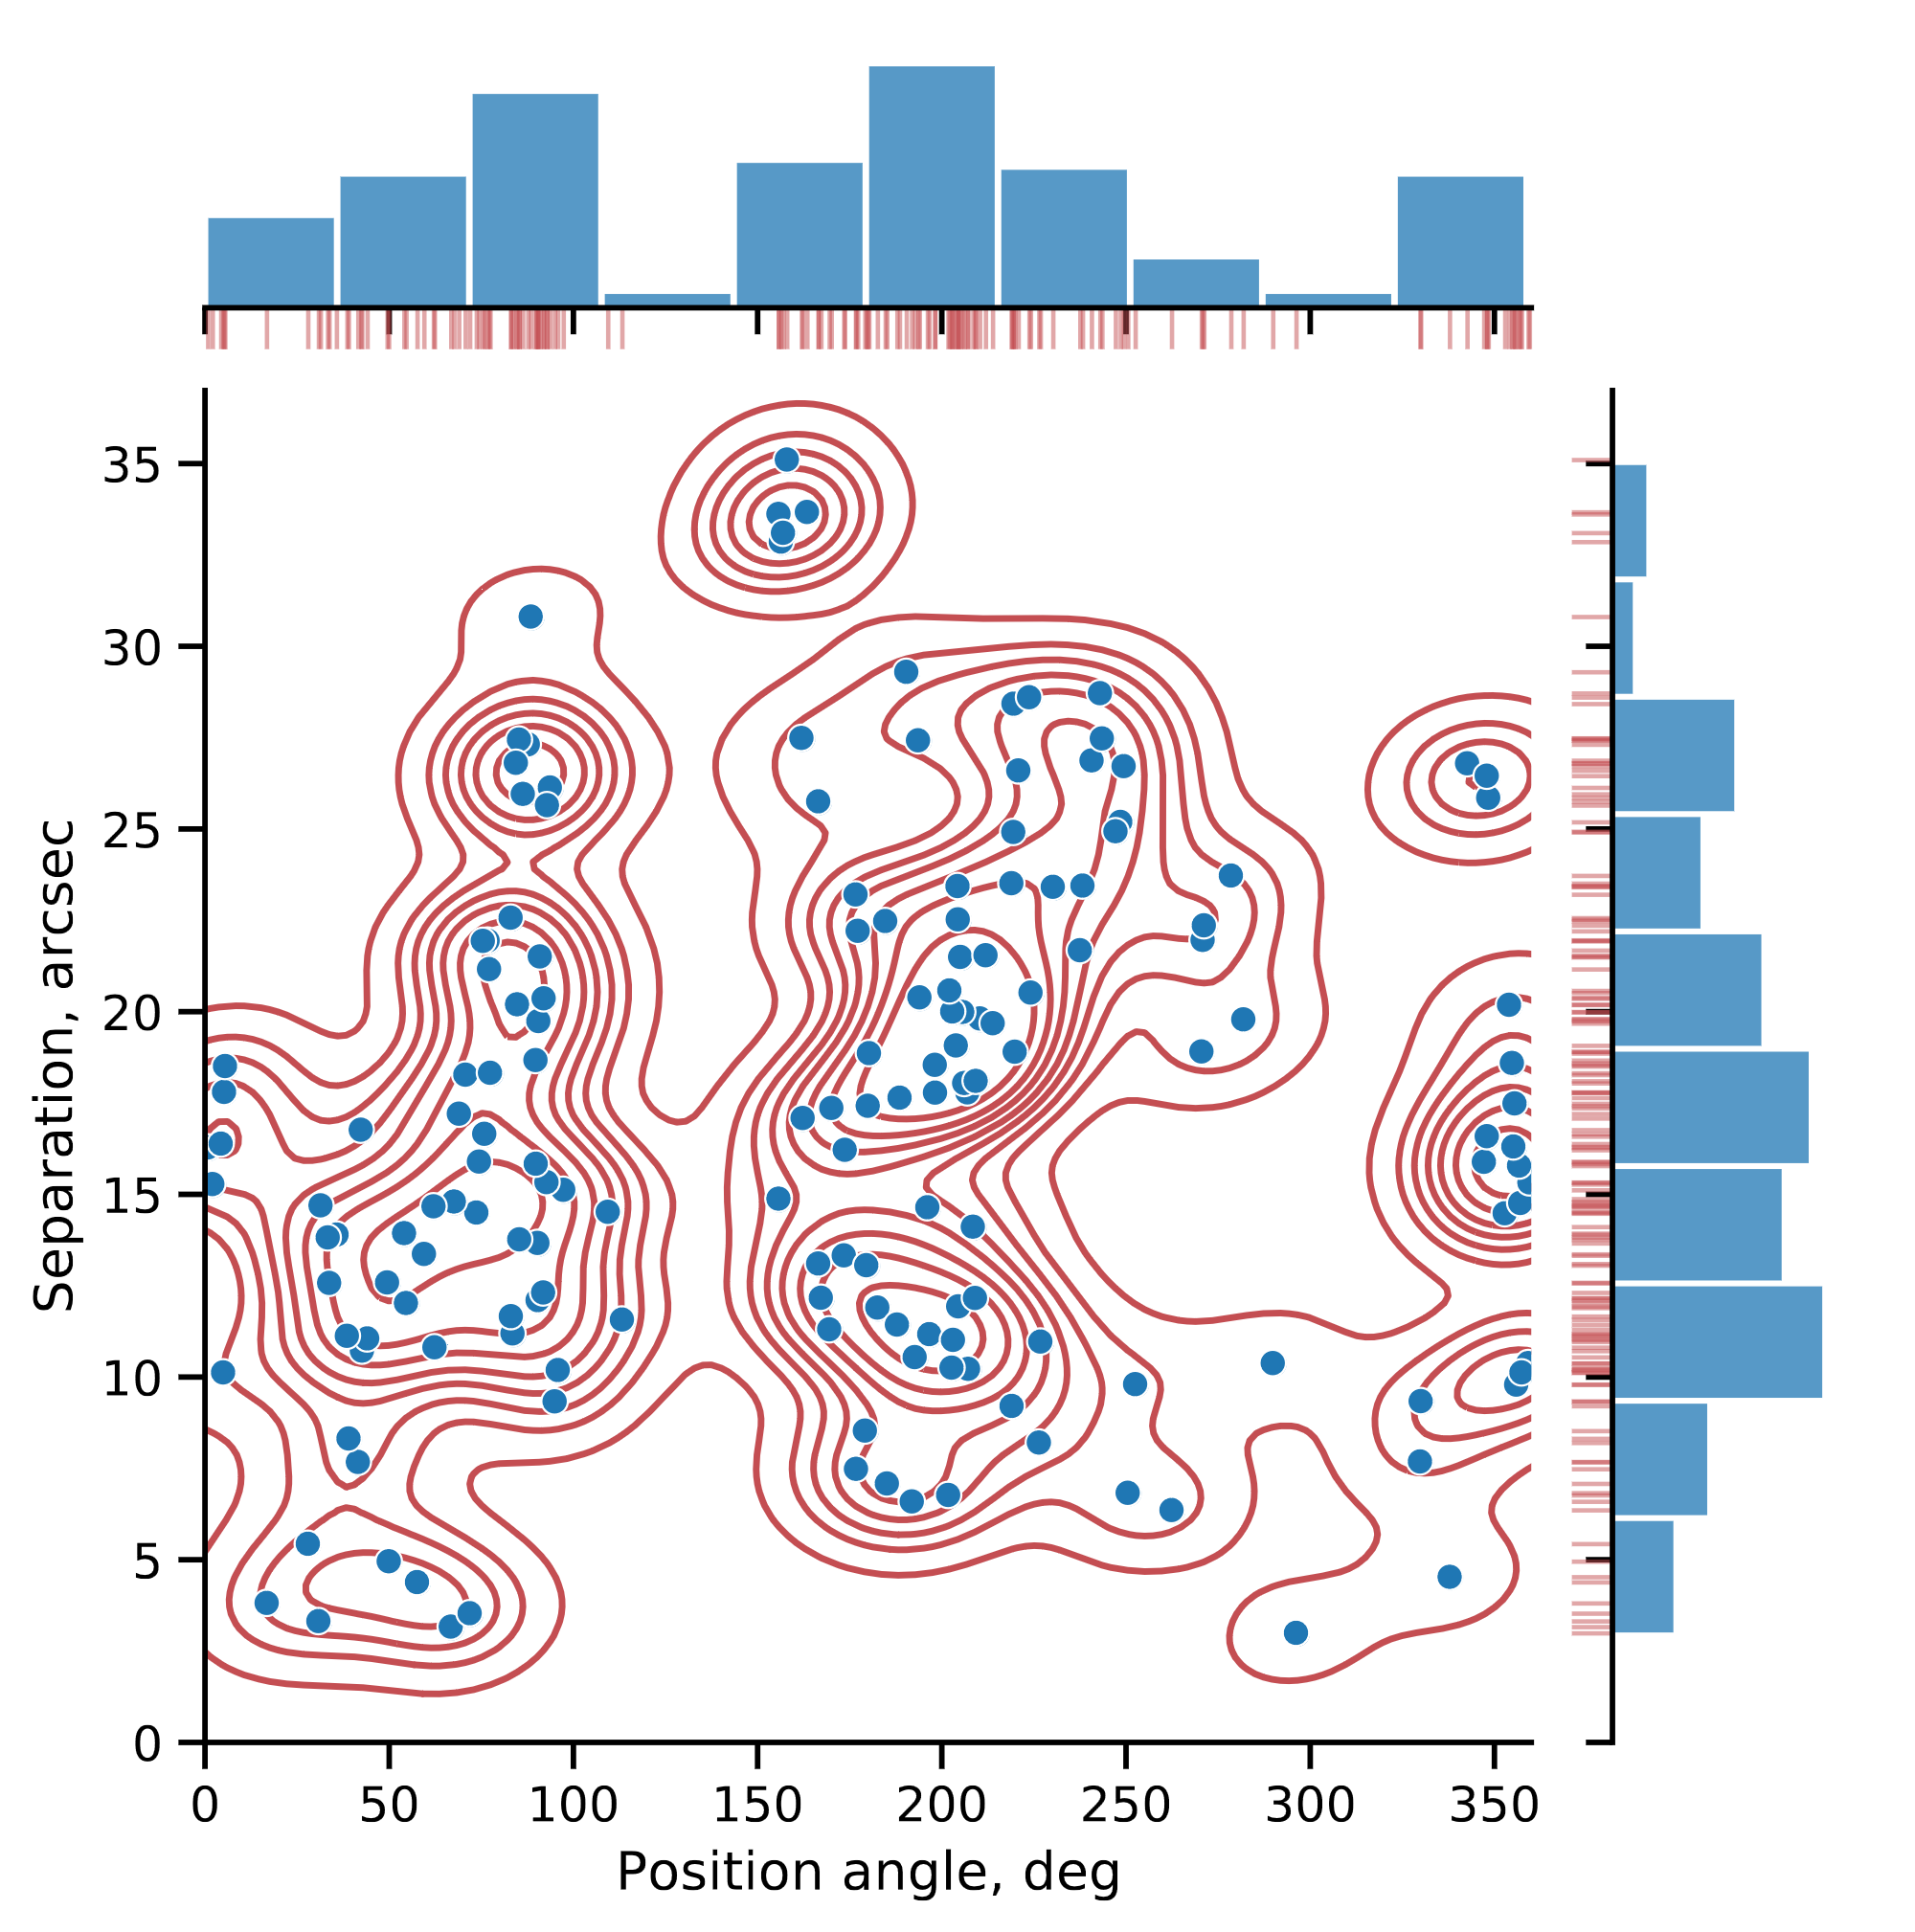
\includegraphics[width=0.75\textwidth]{images Chapter 2/C2_nudos_distribucion.png}
    \caption{Distribución de los nudos en la nebulosa M1-67}
    \label{fig:dis_nudos}
\end{figure}

Estos nudos fueron posibles de encontrar gracias a las imágenes del JWST y se encontraron más de 100 nudos. Algunos de estos nudos están muy cercanos a otros por lo que nos hace pensar que están en grupo y algunos otros aparentemente están muy cercanos a la estrella central, pero debemos tomar en cuenta que lo que en realidad vemos es una proyección en el plano del cielo por lo que algunos nudos podrían estar más lejos de lo que se ve en las imágenes o no estar en ciertos grupos cerca de otros nudos. Podemos ver también una cierta simetría en la distribución de estos nudos en toda la nebulosa como vemos en la figura \ref{fig:dis_nudos}, donde la separación es la distancia del nudo a la estrella y la posición angular es tomada en sentido contrario a las manecillas del reloj desde el polo norte de la imagen de M1-67.

\section{Observaciones con HST}

Para las observaciones con HST utilizamos los datos del proyecto HLA, los cuales son tipo imagen en formato FITS con un nivel de calibración 3.  Se observó en el filtro F656N utilizando la cámara WFPC2 para ver la emisión en \unit{H\alpha}. Este archivo tiene un tiempo de exposición de \SI{4200}{sec}.  

\begin{figure}[h]
    \centering
    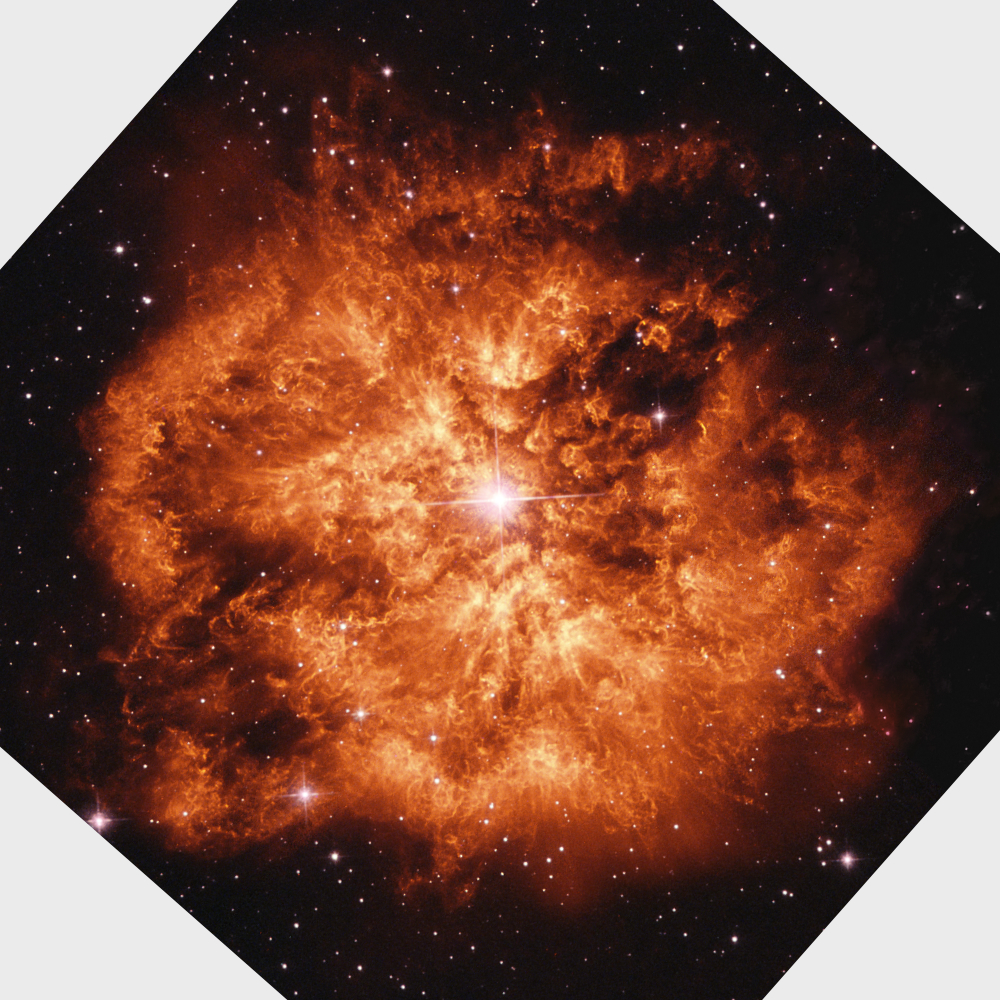
\includegraphics[width=0.8\textwidth]{m1-67-comp-full-hst.jpg}
    \caption{Imagen de M1-67 con el filtro \unit{H\alpha} .}
    \label{fig:M1-67HST}
\end{figure}

\section{Observaciones con JWST}

Para las observaciones con JWST usamos las observaciones propuestas por Klaus M. Pontoppidan con número de propuesta 2730. Se usaron los filtros F090W, F150W, F210M, F335M, F444W, F470N de la NIRCAM con un tiempo de exposición de \SI{2662.72}{s}. Estos archivos son tipo imagen de nivel 3 y están en formato FITS.


\begin{figure}[h]
    \centering
    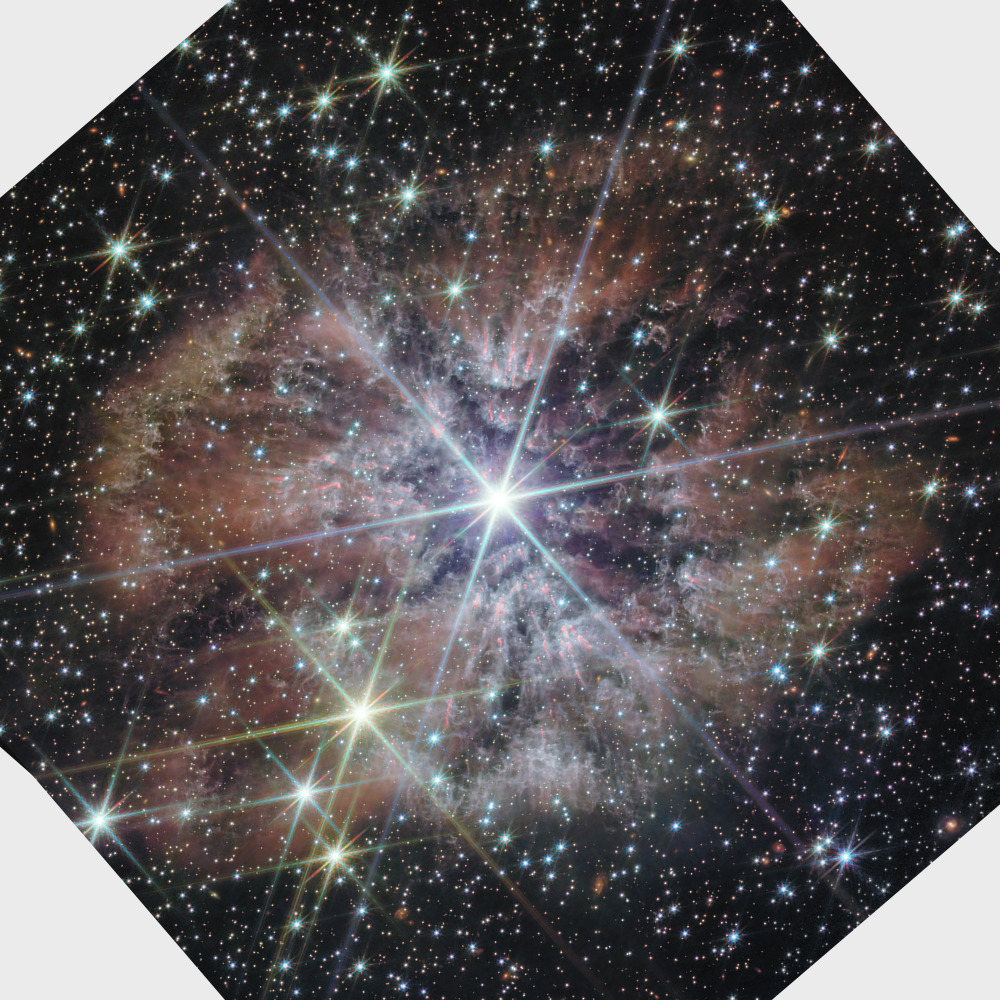
\includegraphics[width=0.8\textwidth]{M1-67-JWST.jpg}
    \caption{Imagen de M1-67 con JWST}
    \label{fig:M1-67JWST}
\end{figure}

\section{Estimación de la densidad ionizada a partir del brillo superficial de \unit{H\alpha}}

Para estimar la densidad ionizada, usamos primero la definición de medida de emisión (EM por sus siglas en inglés)
\[EM=\int_z n_i n_edz\] donde en este caso estaremos integrando sobre nuestra línea de visión. Esta EM depende tanto de la densidad de electrones como de iones, pero en nuestro caso vamos a considerar un equilibrio de ionización entre el flujo fotoevaporativo y el viento estelar, por lo que $n_e=n_i$.

\begin{figure}[h]
    \centering    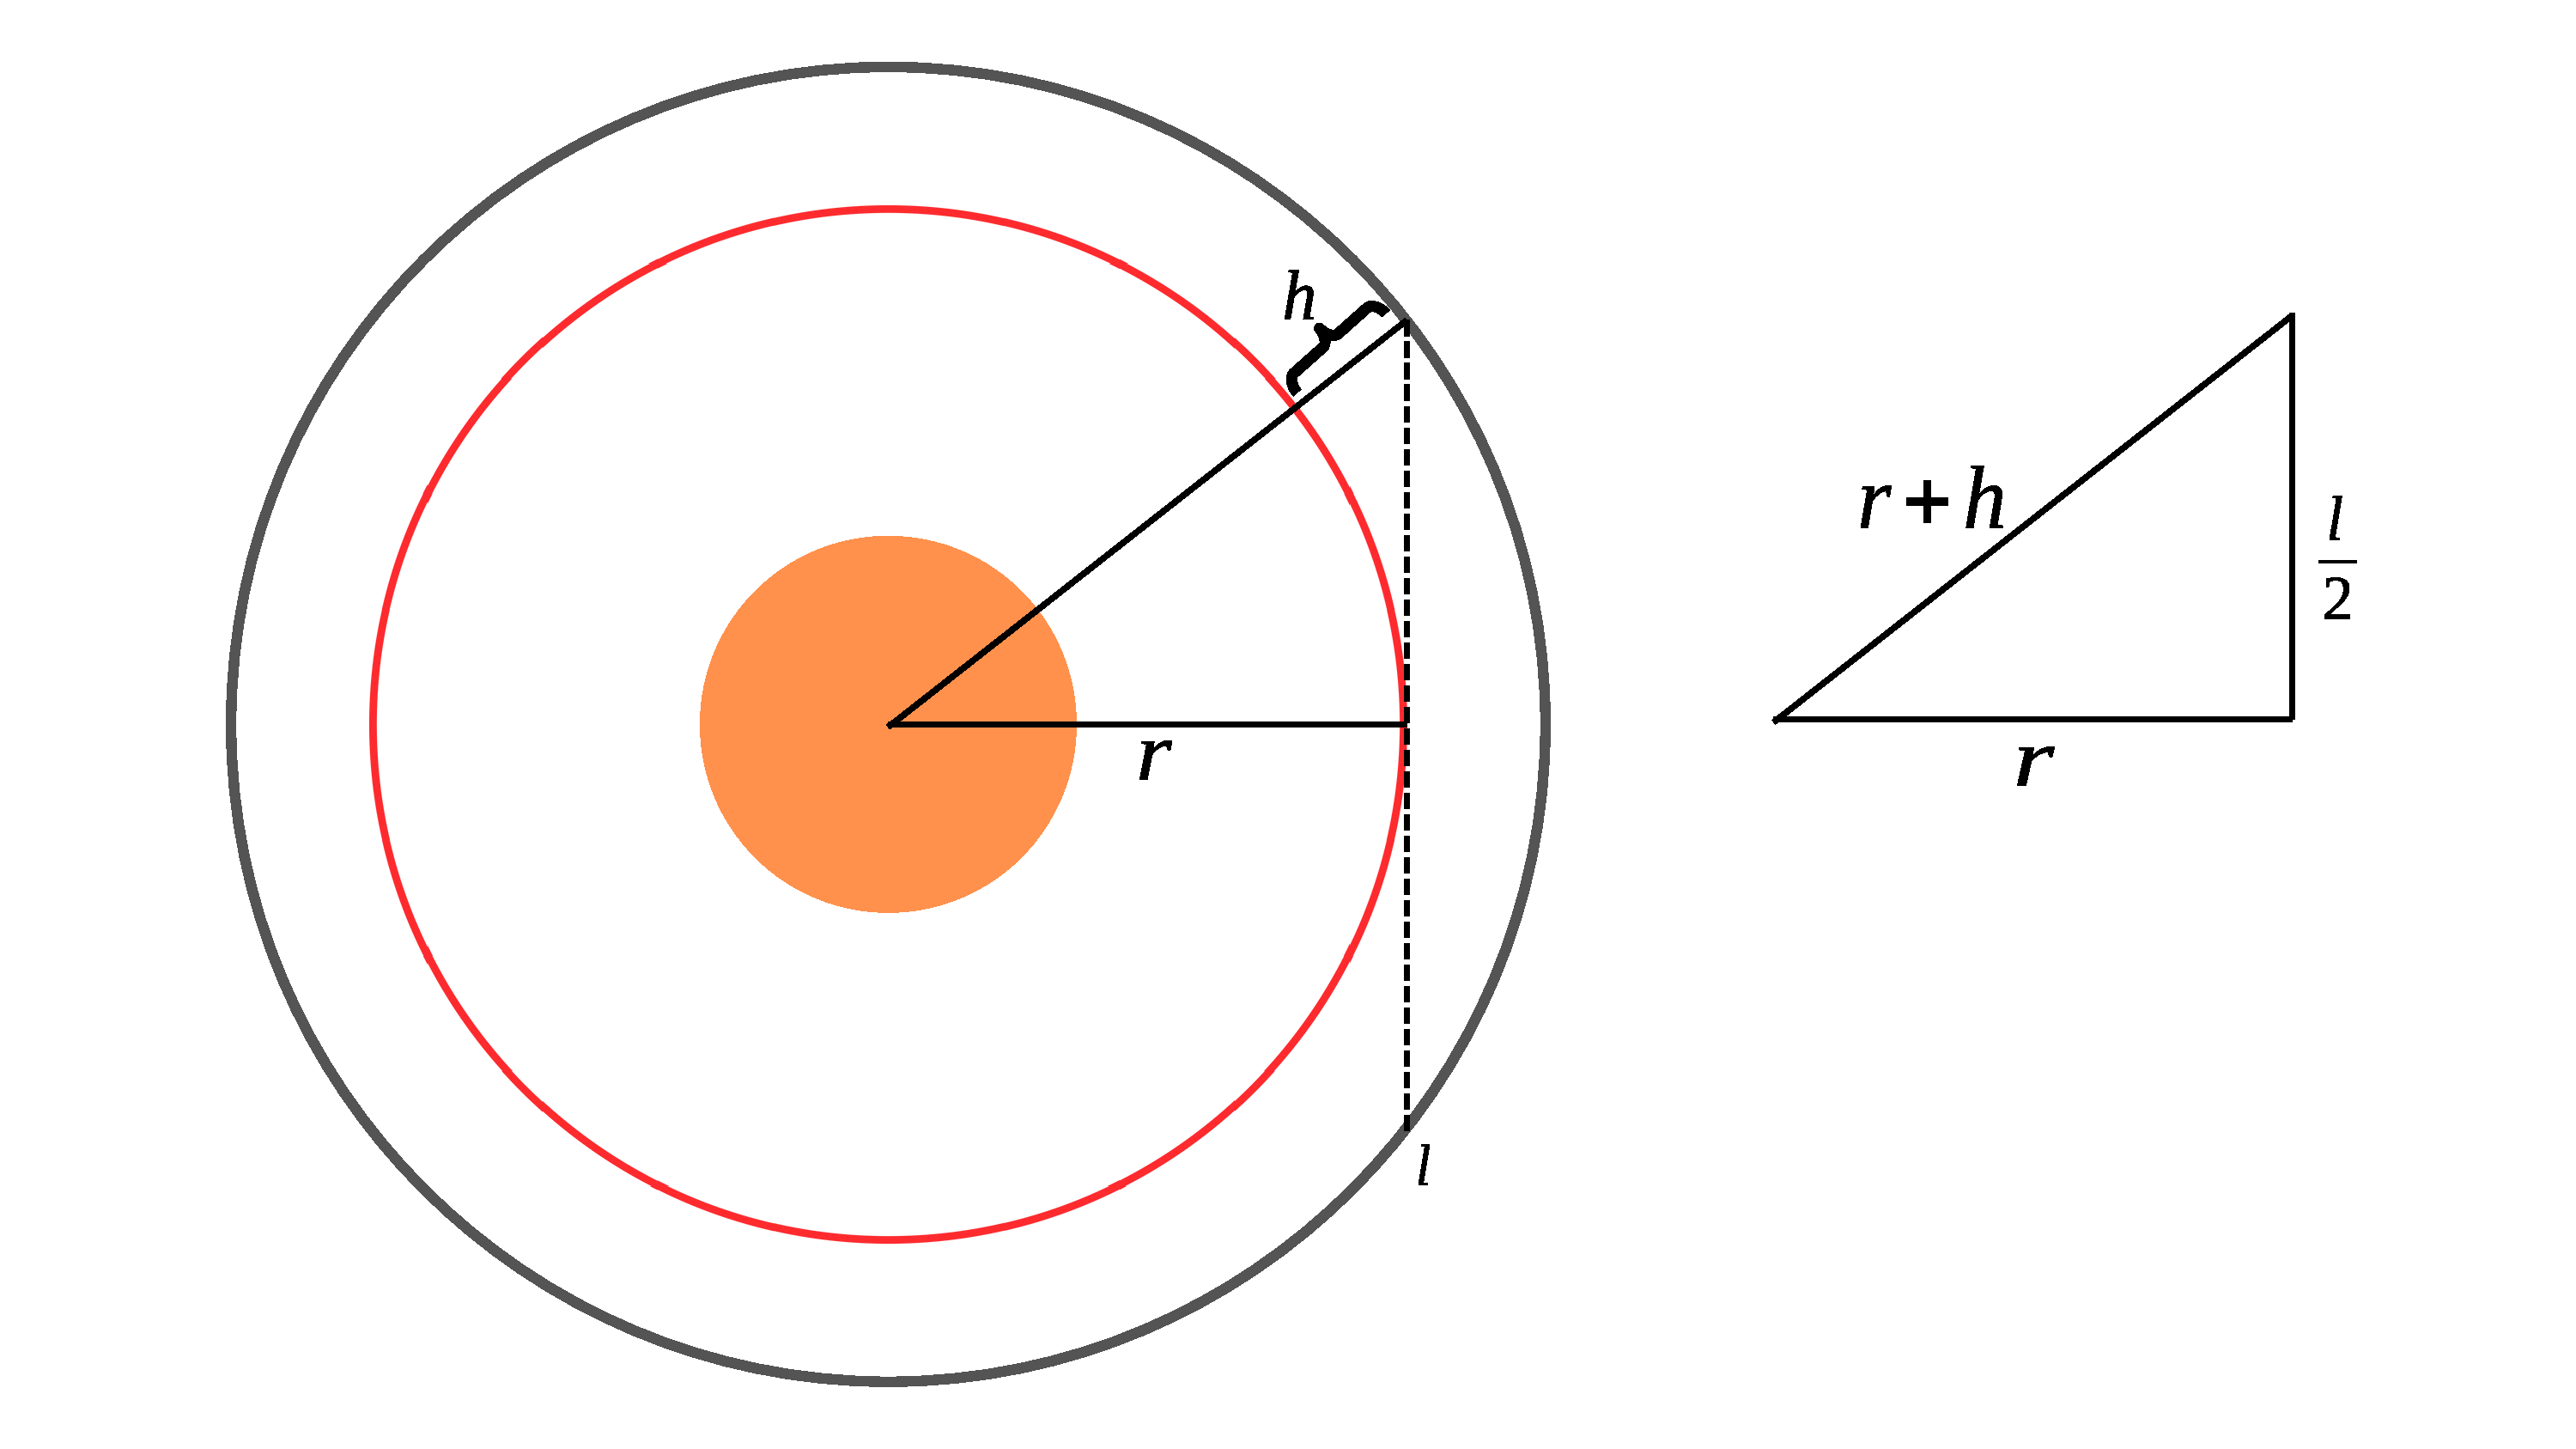
\includegraphics[width=\textwidth]{artesanales/ImgFi01-4.pdf}
    \caption{Como la medida de emisión se mide a lo largo de la línea de visión, vamos a tener un máximo en la línea punteada $l$ y si consideramos una simetría esférica vamos a tener esta configuración donde $h$ será el ancho de la cáscara chocada, $r$ el radio del centro del glóbulo hasta donde inicia el flujo fotoevaporativo chocado y $h<r$.}
    \label{fig:EM}
\end{figure}

Si suponemos una simetría esférica entre esta interacción del flujo fotoevaporativo y el viento estelar, podemos tomar, por geometría, que
\[EM=2\sqrt{2rh}n^2.\]


Esto ya que de la figura \ref{fig:EM} tenemos que por geometría $r^2+\Big(\frac{l}{2}\Big)^2=(r+h)^2=r^2+2rh+h^2\approx r^2+2rh\Rightarrow l=2\sqrt{2rh}$. De esta manera, usando la EM tenemos que \[n=\sqrt{\frac{EM}{l}}=\sqrt{\frac{EM}{2\sqrt{2rh}}}\] 

\subsection{Uso de la EM a partir de las observaciones} \label{Subsec : EM}

Para medir la EM a partir de las observaciones en \unit{H\alpha} usamos lo siguiente. Primero para la intensidad $I$ en unidades cgs (\SI{}{fotones.s^{-1}.cm^{-2}.sr^{-1}}) tenemos que
\[\frac{I}{cgs}=\int \frac{f_{H\alpha}\alpha_\beta n_e n_p}{4\pi}dz\] donde $f_{H\alpha}$ es la fracción de todas las recombinaciones a los niveles $n\le 2$, $\alpha_\mathrm{B}$ el coeficiente de recombinación para el caso B, $n_e$ la densidad electrónica, $n_p$ la densidad de iones y todo esto se integra a lo largo de la línea de visión. Si consideramos como constantes tanto a la fracción de fotones como al coeficiente de recombinación a lo largo de la línea de visión entonces tenemos que
\[\frac{I}{cgs}=\frac{f_{H\alpha}\alpha_\mathrm{B}}{4\pi}\int n_en_pdz=\frac{f_{H\alpha}\alpha_\mathrm{B}}{4\pi} EM \approx \frac{\SI{1.17e-13}{}}{4\pi}EM.\]
Por otro lado para el brillo $B$ en las observaciones con  HST tenemos que multiplicar por 0.0137 para tener el brillo en unidades  \SI{}{erg.s^{-1}.cm^{-2}.sr^{-1}}, por lo que para comparar con $I$ tenemos que dividir entre la energía de $H_\alpha$
\[\frac{B}{cgs}=\frac{0.0137}{(h\nu)_{\unit{H\alpha}}}\] por lo que podemos conocer la EM a partir de las observaciones como 
\[\frac{\frac{B}{cgs}}{\frac{I}{cgs}}=\frac{\frac{0.0137}{(h\nu)_{\unit{H\alpha}}}}{\frac{\SI{1.17e-13}{}}{4\pi}EM}\Rightarrow EM = \Big(\frac{I}{B}\Big)\frac{4\pi 0.0137}{\SI{1.17e-13}{}(h\nu)_{\unit{H\alpha}}}\] como todo está en unidades cgs, entonces nuestra EM tendrá unidades de \SI{}{cm^{-5}}.

Es importante mencionar que en este caso estamos considerando que $l$ es perpendicular a el eje de simetría considerado en el modelo. 

Si consideramos que el eje de simetría del glóbulo tienen un ángulo $i$ con respecto a una línea perpendicular a nuestra línea de visión como se ve en la figura \ref{} y si además  suponemos que tenemos una densidad máxima $n_0$ en el eje de simetría, el cual decae en promedio con el ángulo como $\cos^{1/2} i$, entonces tendríamos  una densidad \[n_i = n_0\cos^{1/2} i\]

\section{Ajustando el modelo a los perfiles de brillo radial}\label{Sec: Ajuste de modelo}

Gracias a la gran resolución del JWST podemos saber donde se encuentran estos nudos exactamente. Con esto podemos identificar el eje de simetría que une al nudo con la estrella y con ello identificar mejor cual es la parte neutra del nudo y cual es la cascara chocada.

Para saber estos tamaños graficamos la intensidad de cada píxel como función de la distancia al centro del nudo. Para esto consideramos solo los píxeles que están a una distancia máxima de \SI{1.5}{\arcsecond} y a un ángulo máximo de 60 grados con respecto al eje de simetría.

A estos puntos les ajustamos dos gaussianas y una constante. La primer gaussiana será centrada en cero, que es el centro del nudo. Está primer gaussiana nos dirá el tamaño de la parte neutra del nudo. La segunda gaussiana se ajusta a la cáscara chocada donde tenemos otro pico de emisión debido a las recombinaciones que hay en esa región.

Para este ajuste le dimos menos peso a los píxeles que están mas lejanos del centro del glóbulo y que tienen un gran ángulo con respecto al eje de simetría.

\begin{figure}[h!]
    \centering
    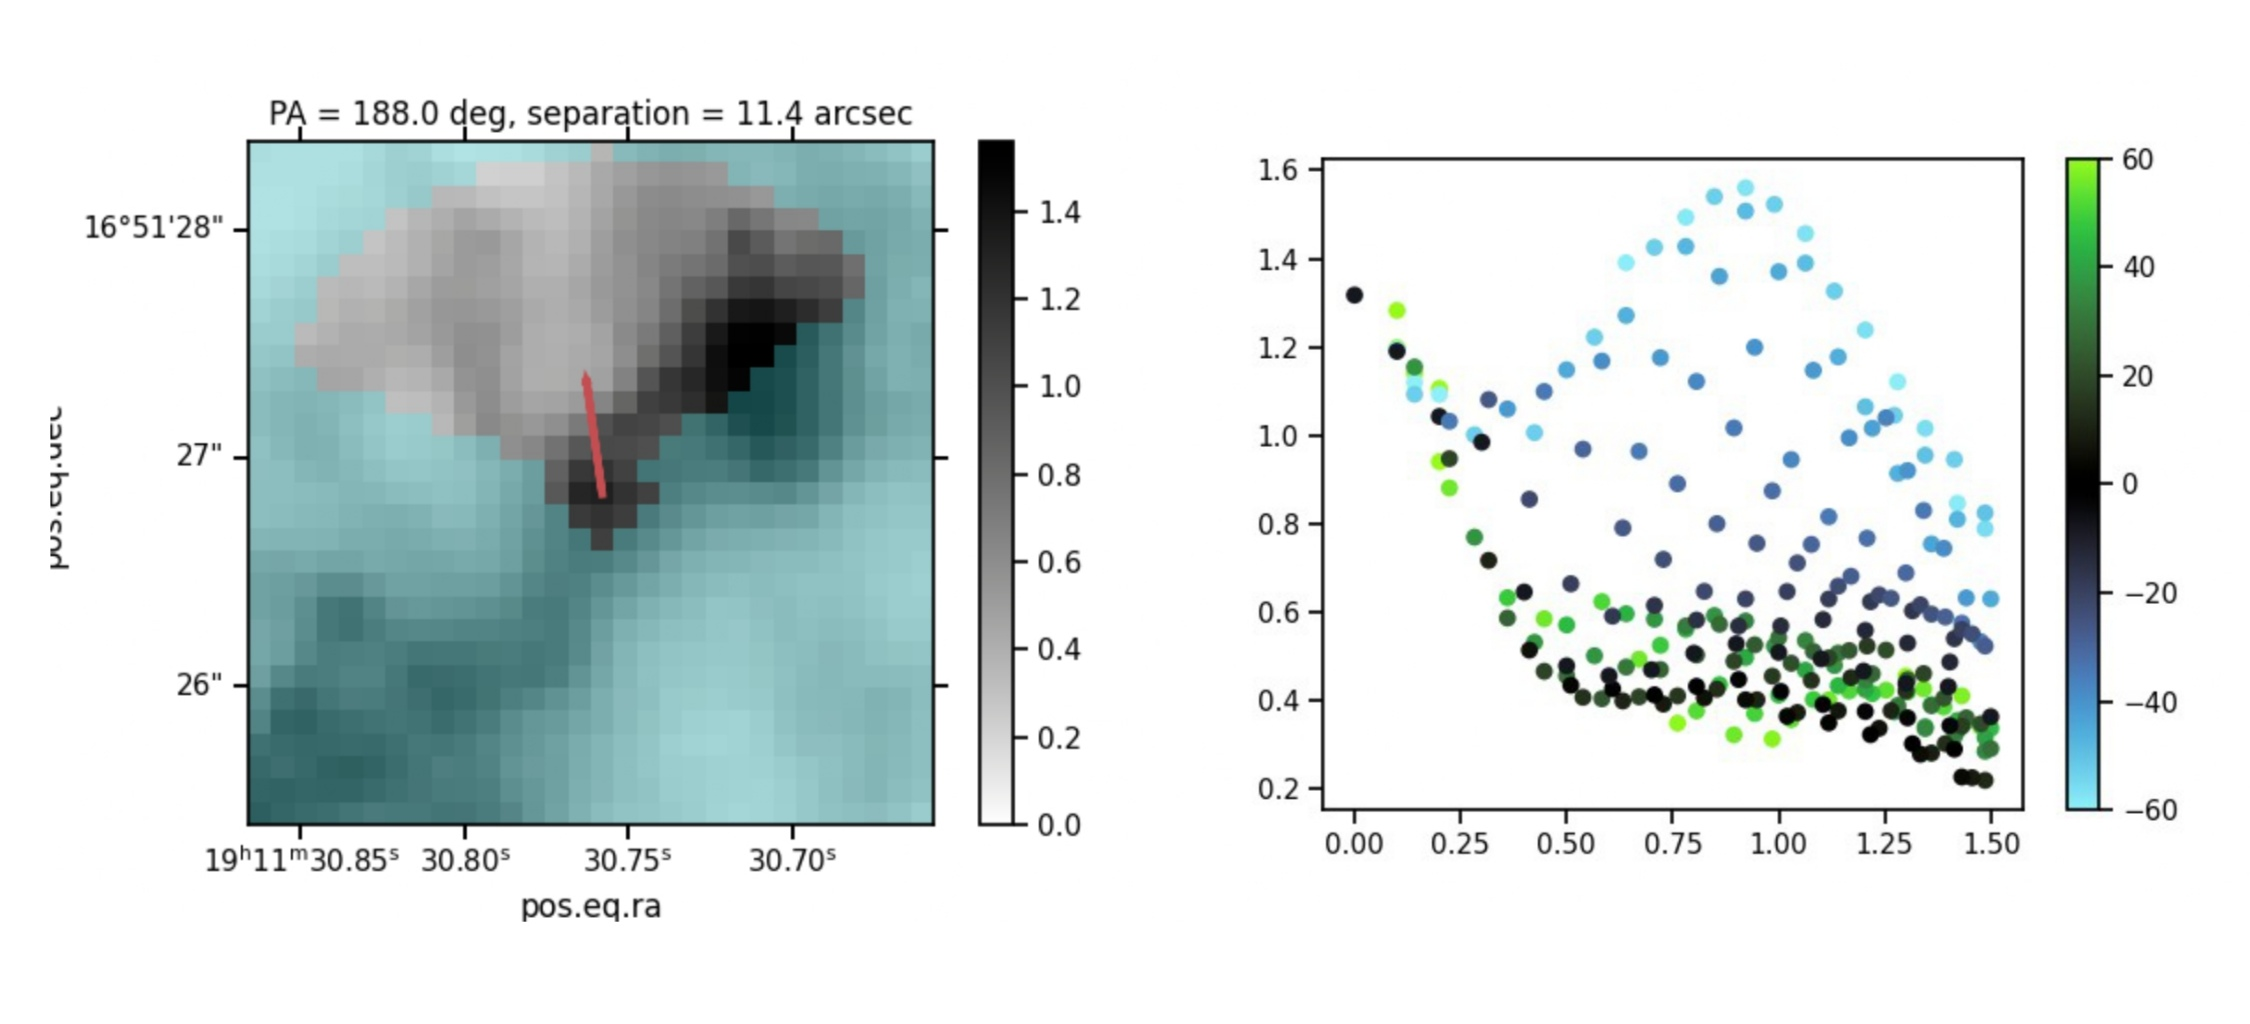
\includegraphics[width=0.75\textwidth]{images Chapter 3/C3_mask.jpg}
    \caption{En la imagen derecha la línea roja representa el eje de simetría que estamos considerando. También vemos la región que solo vamos a considerar en el ajuste, el cual va desde \ang{-60}  (color azul en la imagen derecha) hasta \ang{60} con respecto al eje de simetría (color verde en la imagen derecha) y solo cosideramos una distancia de  \SI{1.5}{\arcsecond} del glóbulo. La parte más oscura en la imagen izquierda representa una mayor intensidad en la emisión de \unit{H\alpha}. En la imagen derecha tenemos la distribución de emisión de \unit{H\alpha} considerando la distancia al glóbulo y el ángulo con respecto al eje de simetría.}
    \label{ejemplo mascara}
\end{figure}

\begin{figure}[h]
    \centering
    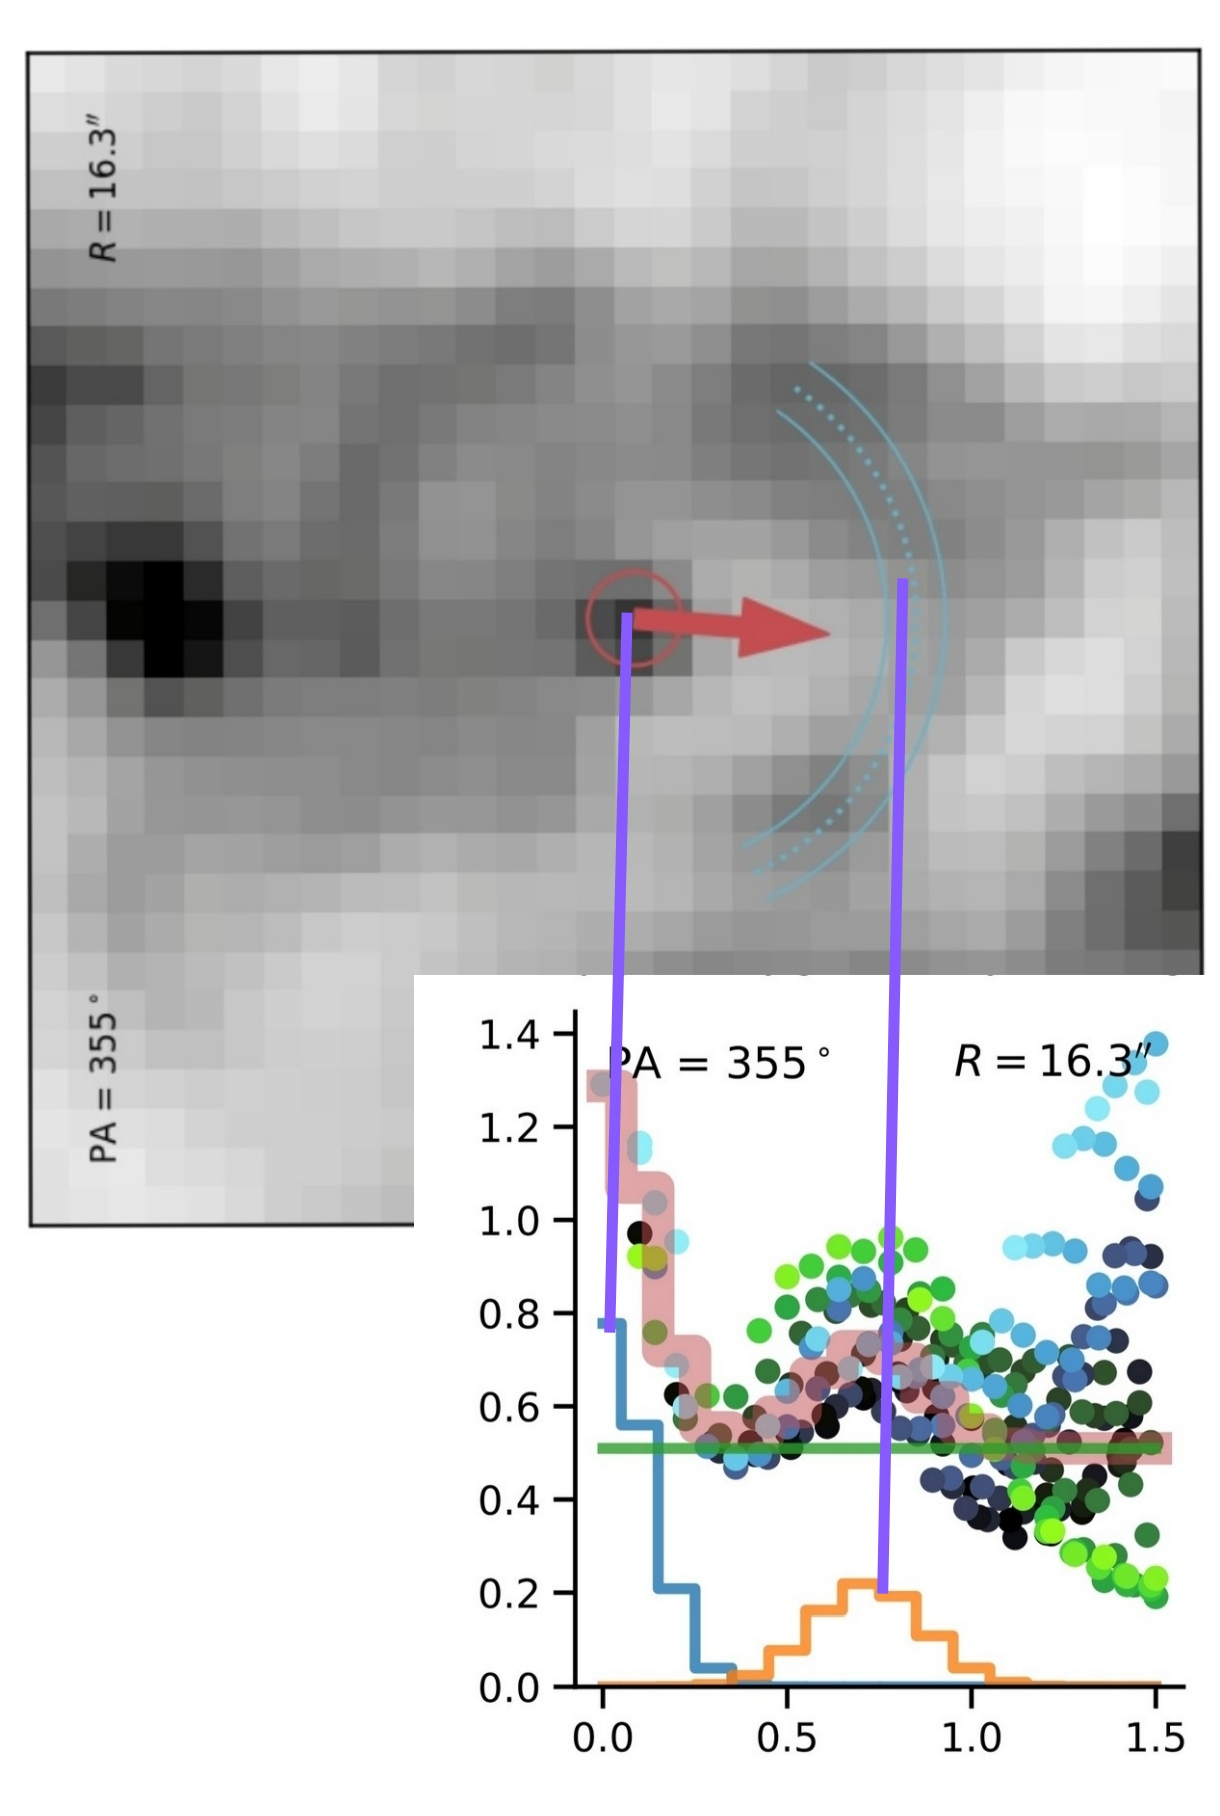
\includegraphics[width=0.75\textwidth]{images Chapter 3/C_3_Ajuste.jpg}
    \caption{Ejemplo del ajuste de dos gaussianas a los perfiles de brillo donde se consideró hasta \SI{1.5}{\arcsecond} de distancia. vemos como se pueden apreciar los dos picos de intensidad tanto en el centro como en la cáscara chocada}
    \label{ejemplo ajuste}
\end{figure}

\section{Estimando la presión RAM del viento estelar}

Como presión externa en este ajuste vamos a considerar solamente la presión RAM del viento estelar por parte de la estrella evolucionada. No vamos a considerar la presión de radiación, magnética ni ninguna otra. 

Para el caso de la presión RAM la vamos a tomar como \[P_{RAM}= \frac{\dot{M}v_\infty}{4\pi R^2}\] donde $\dot{M}$ es la tasa de pérdida de masa por parte de la estrella, $v_\infty$ la velocidad final del viento y $R$ la distancia del nudo a la estrella. Los dos primeros datos están dados en la tabla \ref{tab:parametros WR-124}. Para el caso de la distancia lo que en realidad vemos es una distancia proyectada en el plano del cielo por lo que en un principio requeriría de un ajuste al ángulo en el que se encuentra pero eso lo haremos más adelante.

\begin{figure}[h]
    \centering
    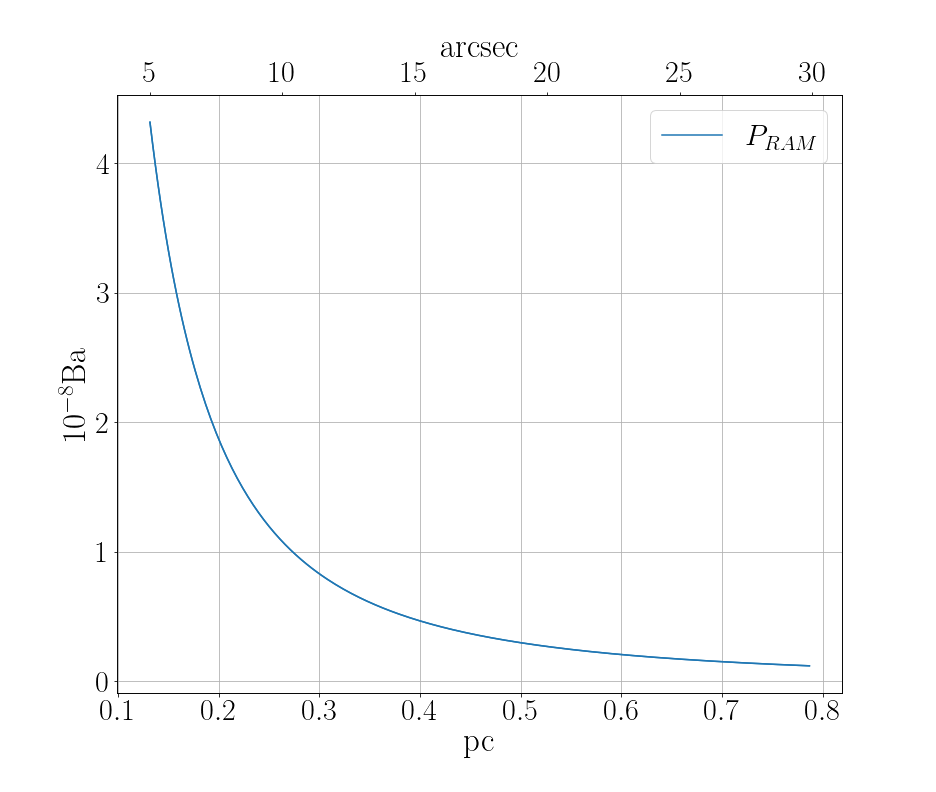
\includegraphics[width=0.8\textwidth]{images Chapter 3/C3_PRAM.png}
    \caption{Presión RAM del viento estelar como función de la distancia en parsec}
    \label{P_RAM}
\end{figure}

\section{Estimando la tasa de foto ionización}

En este caso vamos a considerar las reacciones que están dadas por la siguiente forma 
\[H^0+ h\nu \longleftrightarrow H^+ + e\]
y de ellos lo vcmaoa a considerar en equilibrio de ionización

\[n(H^0)\sigma F = n(H^+)n_e\alpha_\mathrm{B}\] donde $n(H^0)$ es la densidad del gas eutro, $\sigma$ la sección recta, $F$ el flujo de fotones ionizantes, $n(H^+)$ la densidad de gas ionizado, $n_e$ la densidad de electrones y $\alpha_\mathrm{B}$ el coeficiente de recombinación, es decir vamos a considerar que el número de recombinaciones es igual al  número de recombinaciones 

\chapter{Resultados}

Se encontraron alrededor de 168 nudos glóbulos en la nebulosa M1-67 los cuales están distribuidos a una distancia de la estrella central de entre 3--\SI{35}{\arcsecond}, aunque esta distancia puede ser en realidad una distancia proyectada para algunos glóbulos.  Estos glóbulos se pueden observar ya sea en grupos o solos como se puede ver en la figura \ref{fig:dis_nudos}. 

El ajuste de las dos gaussianas a los perfiles de brillo se realizó para las observaciones de HST en H$\alpha$  como ya habíamos mencionado antes. Esto se pudo hacer gracias a que sabíamos donde se encontraban los glóbulos, pero debido a que tenemos una menor resolución que en el JWST no fue posible detectar muy bien tanto la parte neutra como la cáscara en todos los casos y en algunos casos quedaba duda si lo que se detectaba era realmente una cáscara, por lo que también se hizo usando una combinación de los filtros f210m, f150w, f335m y f444w del JWST para ver solo la emisión del gas ionizado y comprobar si lo que se había detectado como una cáscara con las observaciones del HST realmente lo era o no.

\section{Medición del radio en la parte neutra}

Por otra parte, como en estos dos casos anteriores tenemos solo la emisión de gas ionizado la medición para los radios de la parte neutra también estaría mal. Por lo que para la medición de la parte neutra se utilizó la combinación de los filtros f150w, f210m y f335m para ver la emisión neutra. 

En este caso ajustamos solo una gaussiana y una constante al perfil de brillo ya que aquí no podríamos ver la cáscara chocada. El ajuste se realizó de la siguiente manera: Dado que el radio del glóbulo en el anterior ajustes tenía un valor medio de \SI{0.14}{\arcsecond} con una variación de $\pm\SI{0.04}{\arcsecond}$ decidimos poner una máscara de \SI{0.2}{\arcsecond} alrededor del pico de emisión y unos conos con un pequeño ángulo de apertura, estos conos son perpendiculares al eje de simetría considerado en el modelo y tienen una longitud de \SI{1.5}{\arcsecond}. Con esta máscara considerada esperamos tener toda la emisión neutra en el círculo pequeño que consideramos, los conos nos servirán para calcular mejor la constante ajustada.  

\section{Glóbulos descartados}\label{Bad globules}

A pesar de tener una buena cantidad de glóbulos para aplicar a este modelo no se usaron todos por diferentes razones. 

Algunos de ellos tenían un mal ajuste debido a la gran estructura de la nebulosa, había estrellas de fondo o se veían afectados por la difracción del telescopio.  Debido a esto en algunos casos no se alcanzaba a detectar bien la parte neutra o la cáscara chocada y en algunos casos la detección de estas regiones estaban mal en cuanto a sus tamaños.  Para esto ocupamos las observaciones en los dos telescopios ya que para el caso de las observaciones con el HST, que tiene menor resolución, se fijaba más en las grandes estructuras por lo que en algunos ajustes se veían afectados por la gran estructura de la nebulosa o estrellas de fondo. Sin embargo, debido a que las observaciones con JWST se ven muy afectadas por la difracción del telescopio, algunos glóbulos no fueron tomados en cuenta a pesar de que se pudiera observar una posible cáscara.

\begin{figure}[h!]
    \centering
    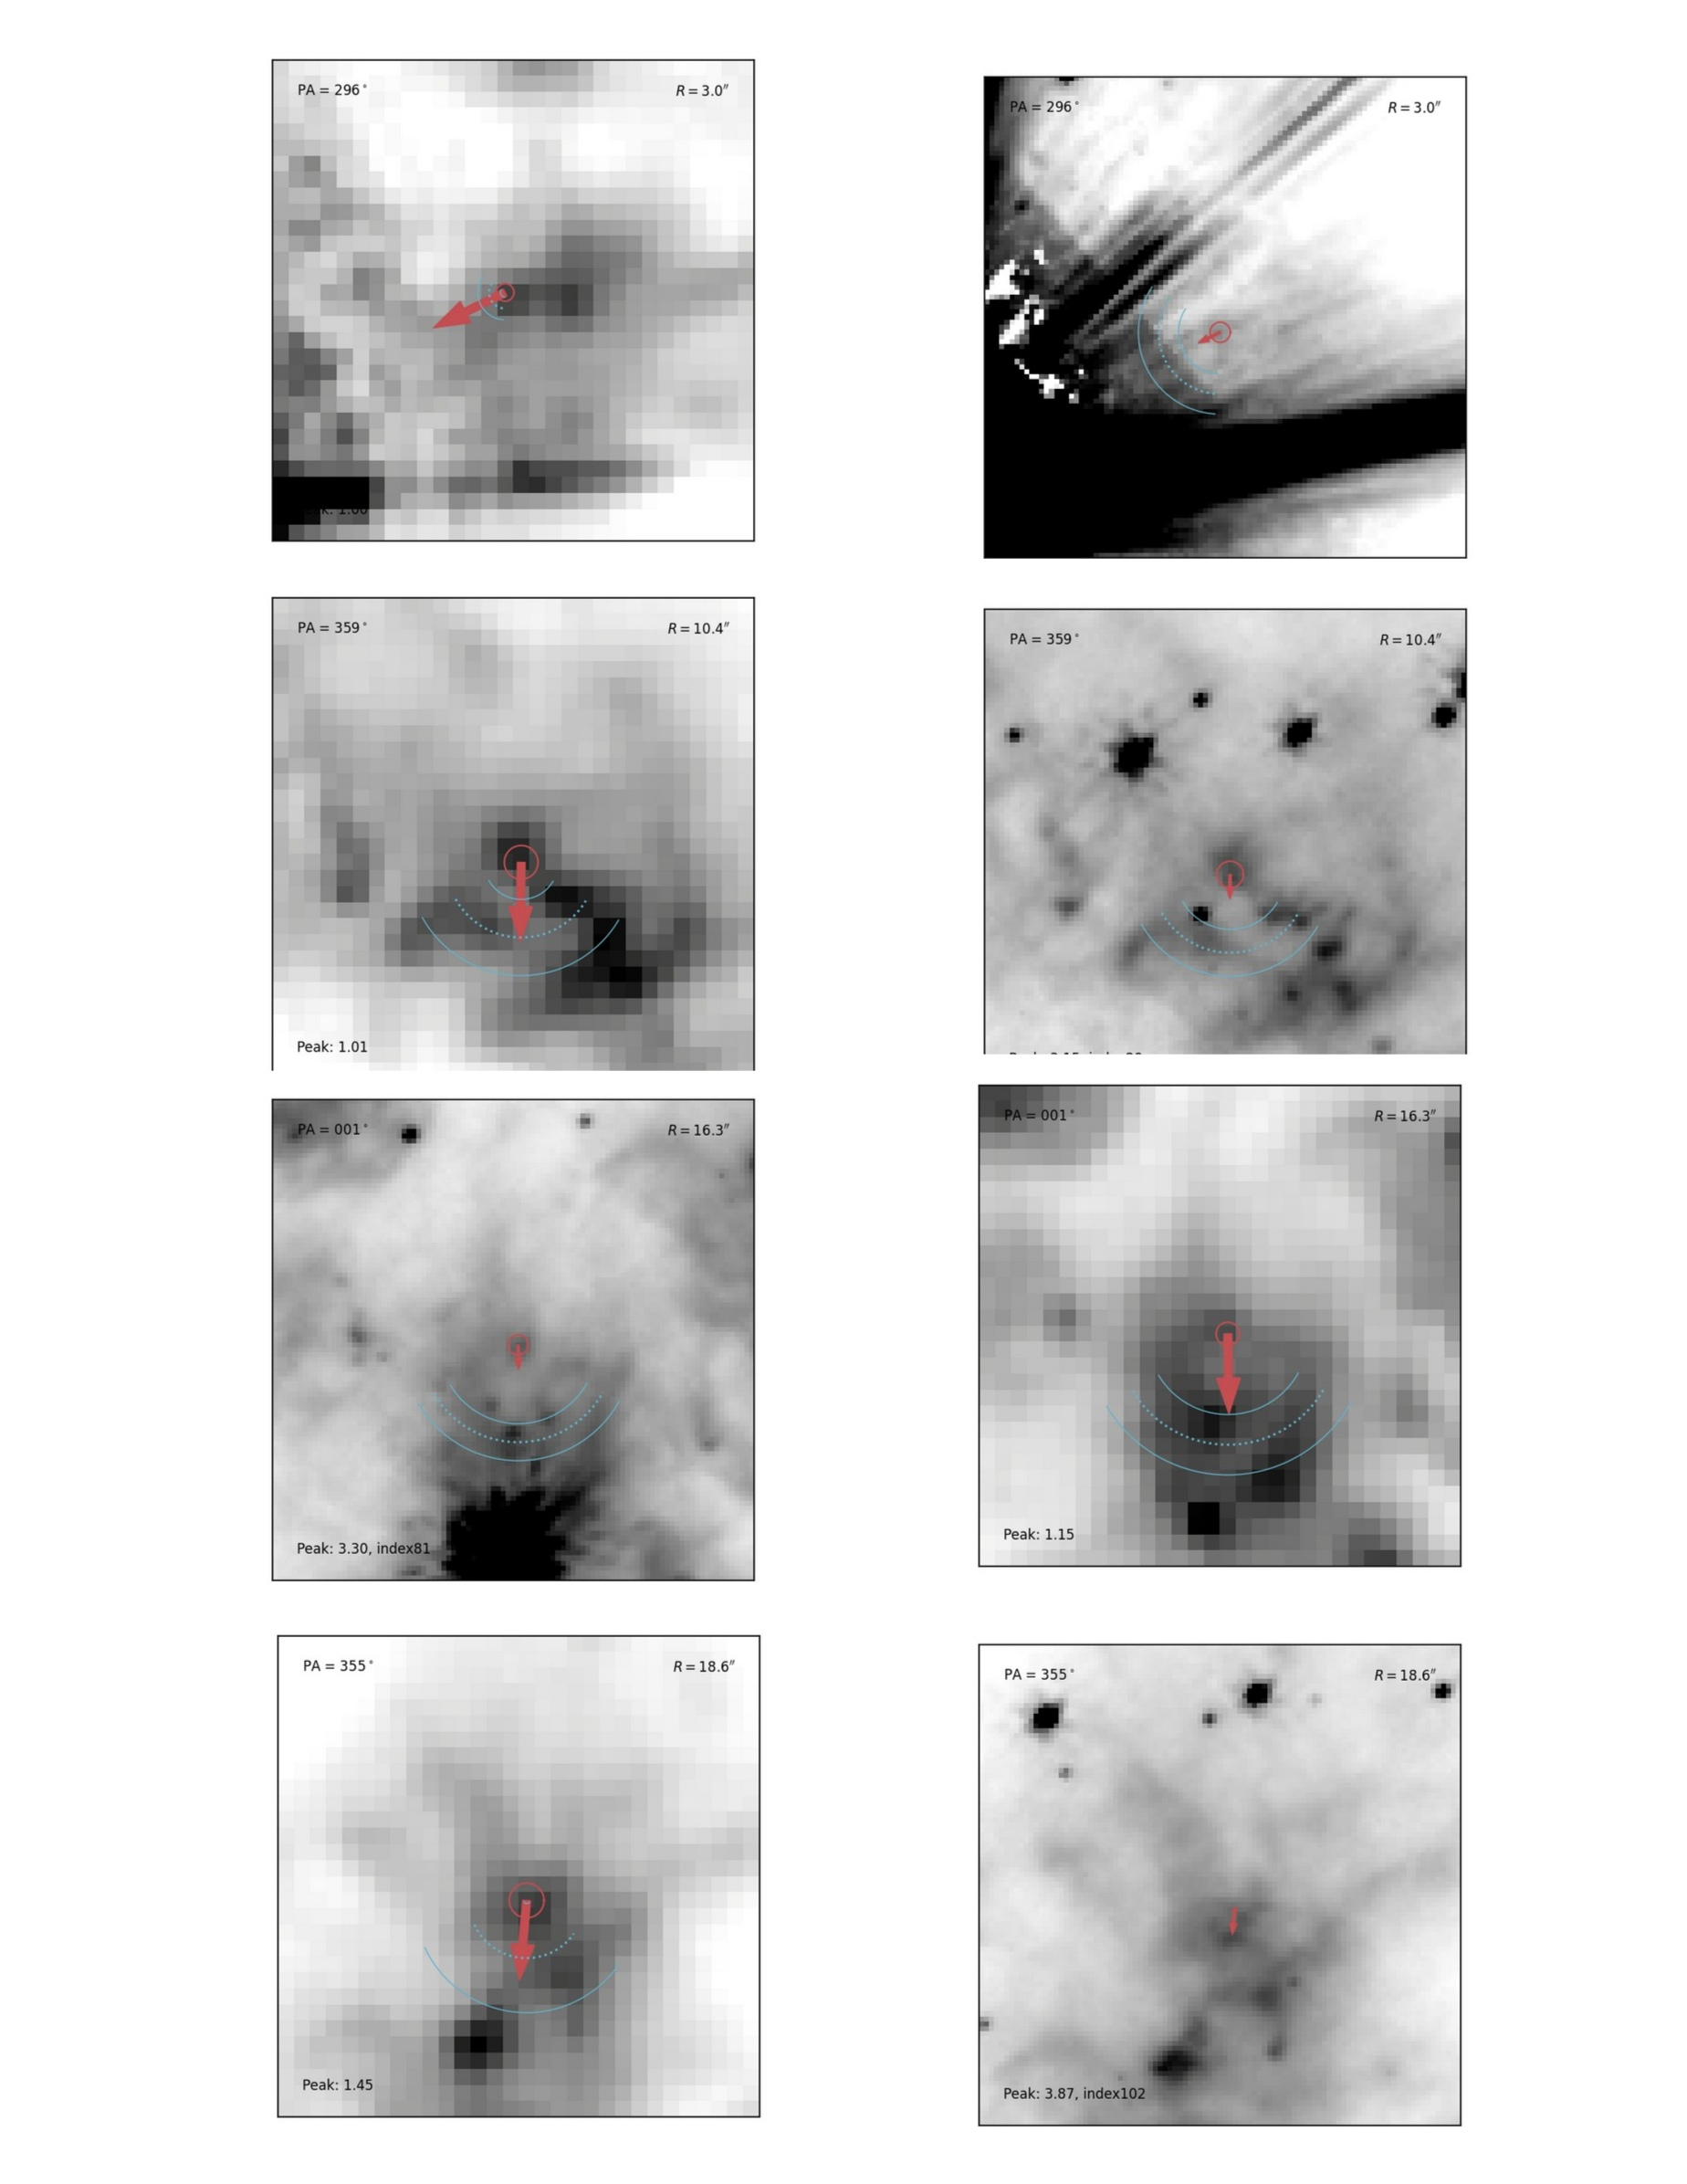
\includegraphics[width=0.75\textwidth]{images Chapter 3/C3_badG.jpg}
    \caption{Ejemplo de glóbulos descartados. Del lado izquierdo es la imagen con el HST y del lado derecho con el JWST. El primer glóbulo es descartado por que se ve afectado por la difracción del telescopio y por la gran estructura de la nebulosa, esto se puede deber a lo cerca que está de la estrella central. En los otros ejemplos vemos como la presencia de fuentes cercanas afecta nuestras estimaciones de posibles cáscaras chocadas en las observaciones.}
    \label{Bad Globules}
\end{figure}


\section{Ajustes recuperados}

Primero se aplicó el ajuste a los perfiles de brillo con los datos del HST y ya vimos que algunos casos quedaron descartados por distintas razones, pero en otros casos se podía ver una cáscara y no la detectábamos, aplicando el ajuste a los datos del JWST  nos dimos cuenta de esto por lo que se pudieron rescatar algunos glóbulos en los que en un inicio no se había detectado la cáscara. Por otro lado, como ya se mencionó antes, nos ayudó también a detectar los ajustes que aparentemente tenían una cáscara pero no era así.

Para agregar estos glóbulos nos fijamos en las mediciones de los radios de las cáscaras y sus anchos. Como vimos que ambos seguían una buena tendencia de que sus mediciones eran más o menos similares, decidimos agregar estos glóbulos con las mediciones del JWST ya que tienen una mejor resolución.

Con esto tenemos una gran variedad de glóbulos en cuanto a sus diferentes tamaños y distancia a la estrella. 
% poner imagen donde se compara el modelo con los resultados obtenidos

\begin{table}[h]
    \centering
    \begin{tabular}{c c c}
        \toprule
        \multicolumn{3}{c}{Resultados de los buenos ajustes} \\ \midrule
          & Media & Desviación estándar.\\
         Separación & \SI{15.55}{\arcsecond}  & \SI{7.04}{\arcsecond}\\
         Radio del glóbulo & \SI{0.14}{\arcsecond} & \SI{0.04}{\arcsecond}\\
         Radio de la cáscara & \SI{0.53}{\arcsecond} & \SI{.17}{\arcsecond} \\
         $n_{cascara}$ & \SI{1372.15}{cm^{-3}} & \SI{397.5}{cm^{-3}} \\
         $P_{cascara}$ & \SI{1.13e-9}{cgs} & \SI{3.24e-10}{cgs} \\
         X & 3.87 & 0.83\\
         $X_P$ & 0.29 & 0.22 \\\bottomrule
    \end{tabular}
    \caption{Valores típicos de los resultados obtenidos y su desviación estándar. X es la fracción de radios $r_1/r_0$  y $X_P$ es la fracción de presiones $P_{RAM}/P_{shell}$. Estos valores son con los resultado obtenidos a partir de las imágenes del HST.}
    \label{tab:mean}
\end{table}

%\section{Estimación de la presión en la zona neutra}

%Usando el modelo hidrodinámico que proponemos podemos calcular cuál es la presión del flujo fotoevaporativo en la base del glóbulo si conocemos el radio del glóbulo y de la cáscara chocada.  

%Para calcularlo tenemos que
%\[\frac{P_{shell}}{P_0}=\frac{P_{shell}}{P_{RAM}}\frac{P_{RAM}}{P_0} \Rightarrow P_0=\frac{P_{shell}}{P_{RAM}}\frac{P_0}{P_{shell}}P_{RAM}\]
%donde $P_{shell}$ es la presión de la cáscara chocada, $P_0$ es la presión del flujo fotoevaporativo en la base del glóbulo y $P_{RAM}$ es la presión del viento estelar. En la ecuación de la derecha, el primer término $\frac{P_{shell}}{P_{RAM}}$ lo podemos calcular usando las observaciones como ya se había mencionado antes, el segundo término $\frac{P_0}{P_{shell}}$ lo podemos obtener del modelo conociendo la razón entre los radios que encontramos y finalmente la $P_{RAM}$ puede ser calculada de las observaciones conociendo la distancia del glóbulo a la estrella.

\section{Buenos ajustes}\label{Good results}

Se pudo obtener mucha información para el caso de los glóbulos en los que se pudieron detectar tanto la parte neutra como la cáscara chocada. 

Con estos buenos ajustes se pudieron conocer los diferentes radios del glóbulo, la densidad en la cáscara chocada usando la EM, la presión de la cáscara y la presión RAM del viento que actúa sobre ellos.

\begin{figure}[h!]
    \centering
    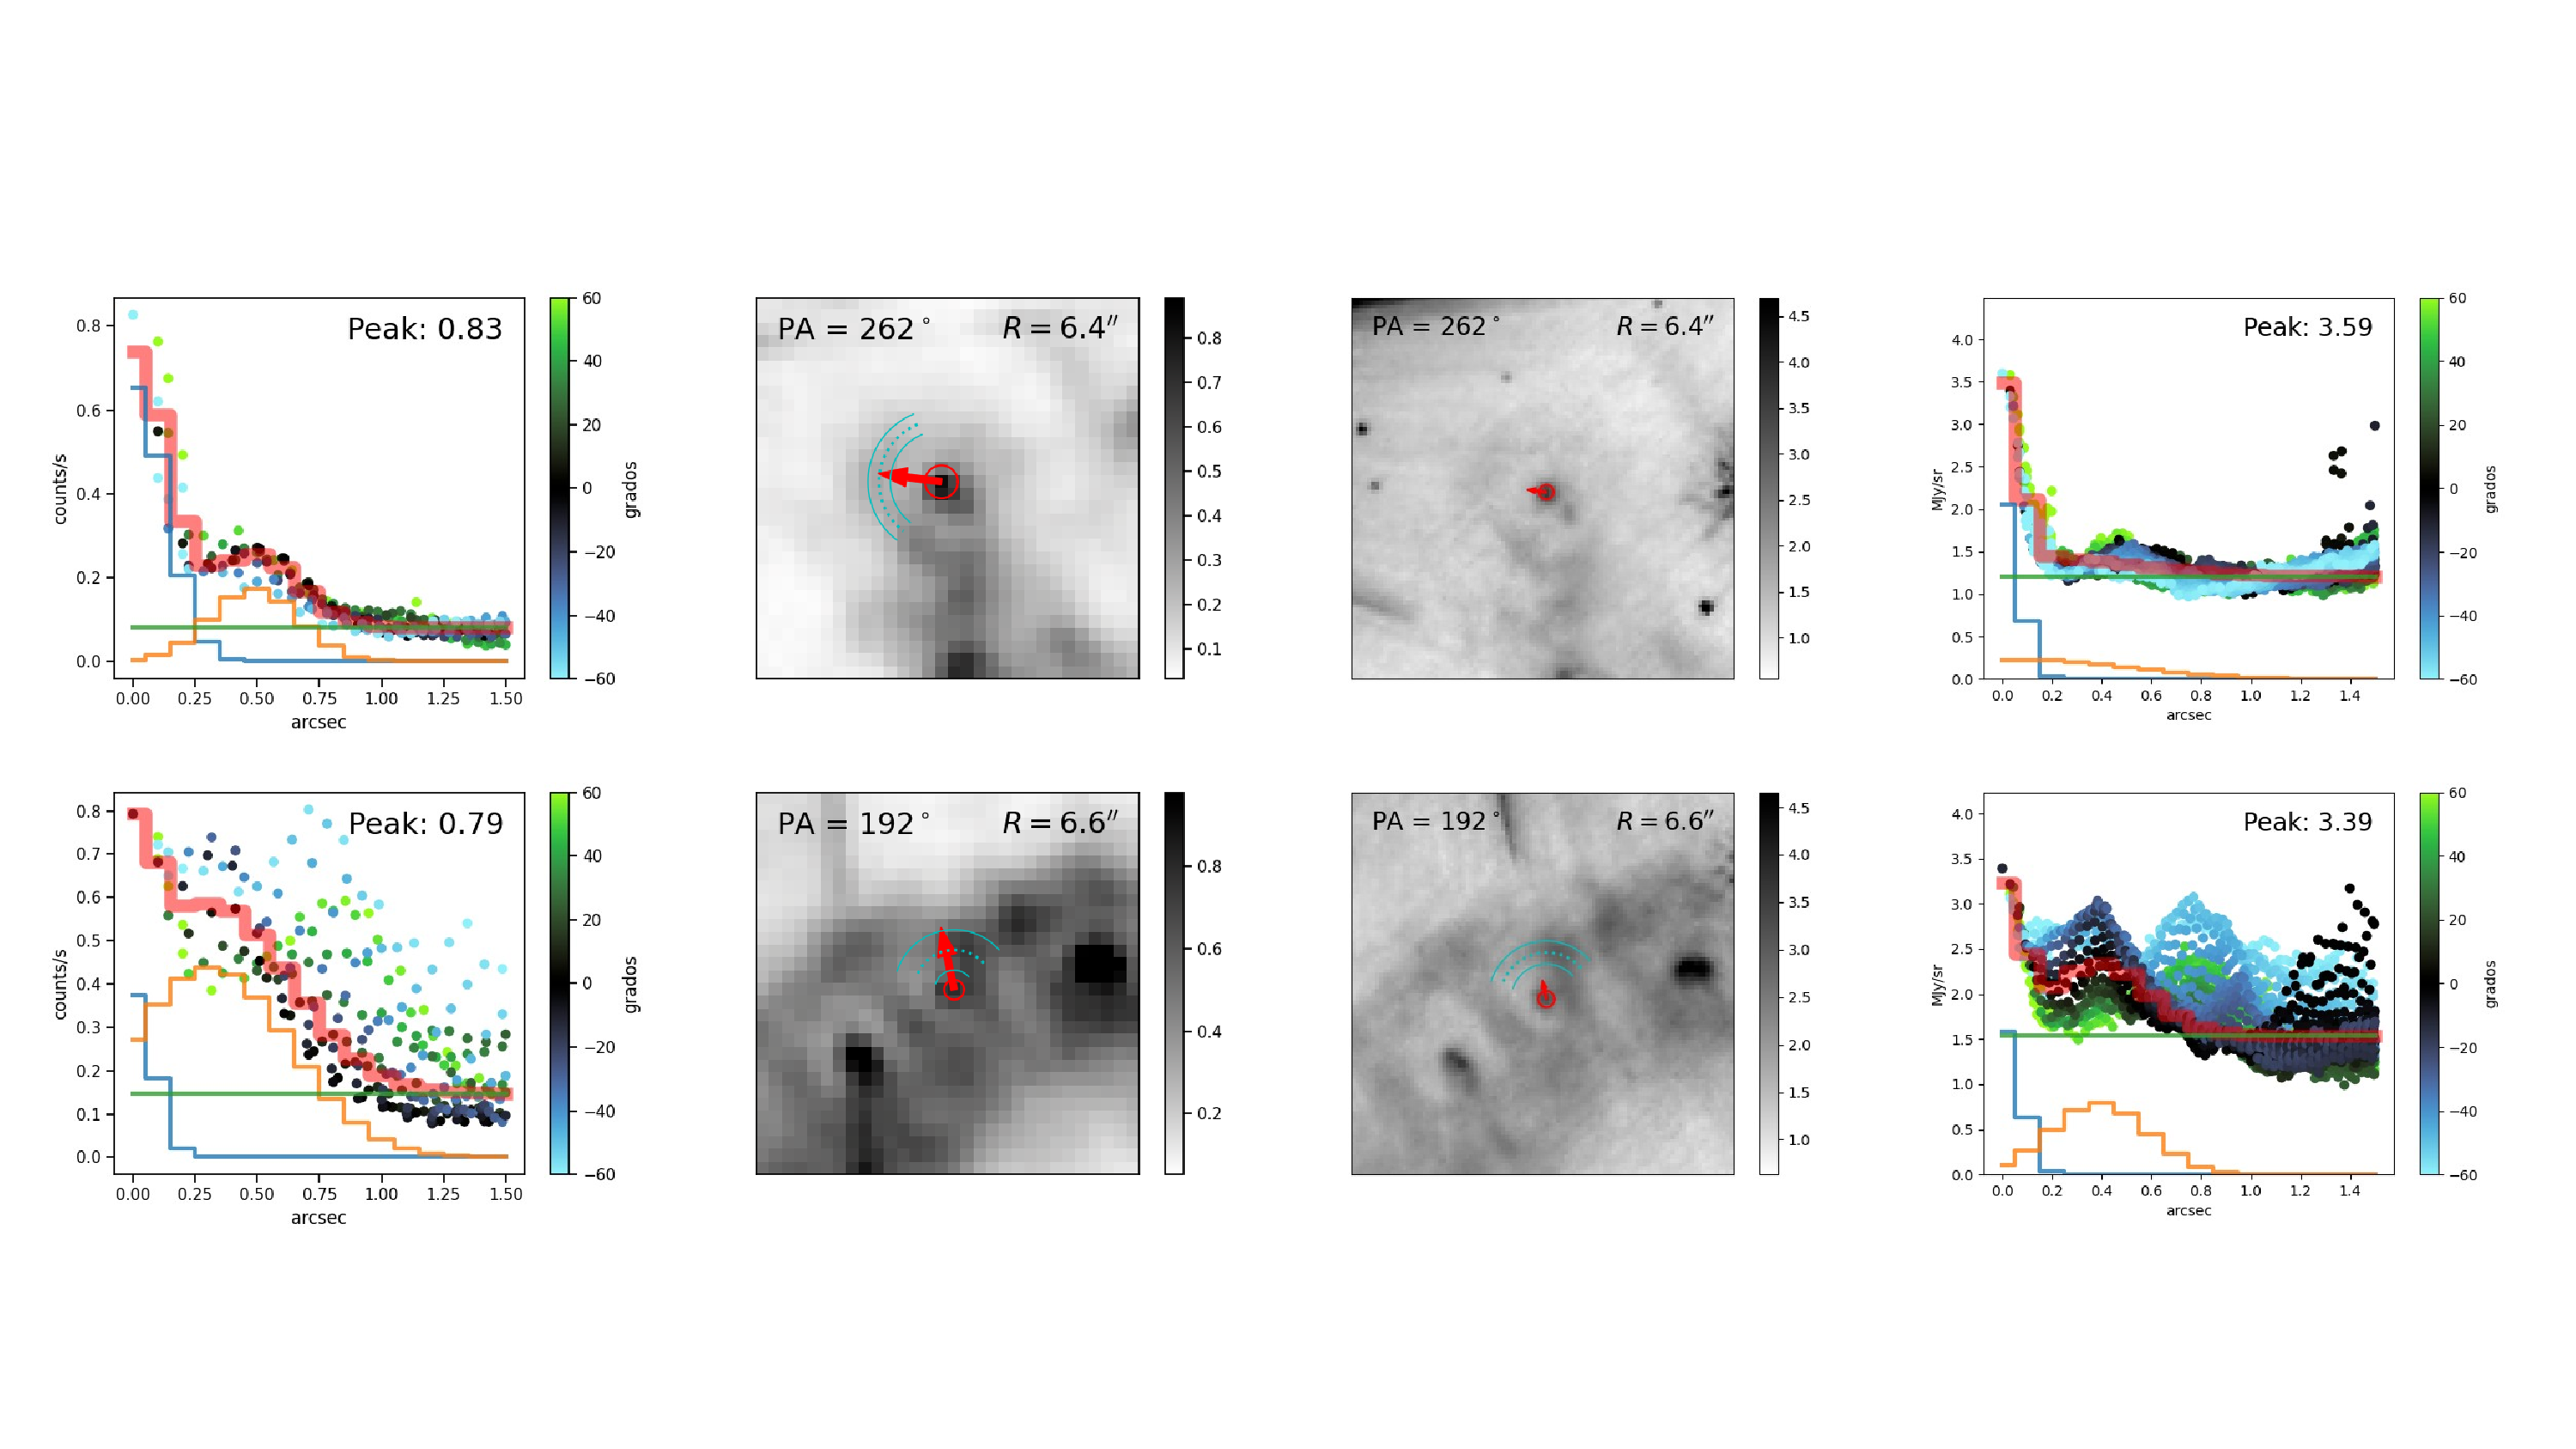
\includegraphics[width=1.2\textwidth]{imagenes Chapter 4/ImgFi011-7.pdf}
    \caption{Ejemplo de buenos ajustes. Las imágenes del lado izquierdo son con el HST y las de l lado derecho con el JWST. Vemos como el ancho de la cáscara chocada son algo similar en ambas observaciones, mientras que el radio en la parte neutra es más pequeña en las imágenes del JWST.}
    \label{Goog G}
\end{figure}

\section{Corrección por proyección}\label{Sec:proyeccion}

Debido a que estamos considerando un equilibrio de presión entre la presión RAM del viento estelar y la presión de la cáscara estos deberían ser iguales, pero como vemos en la gráfica \ref{graf_presion} la presión de la cáscara de los glóbulos es menor que la presión RAM. Esto puede ser debido a que no estamos viendo la distancia real que hay entre los glóbulos y la estrella, por lo que ahora vamos a considerar un ángulo de proyección con el cual las dos presiones ahora estarán en equilibrio.

\begin{figure}[h]
    \centering
    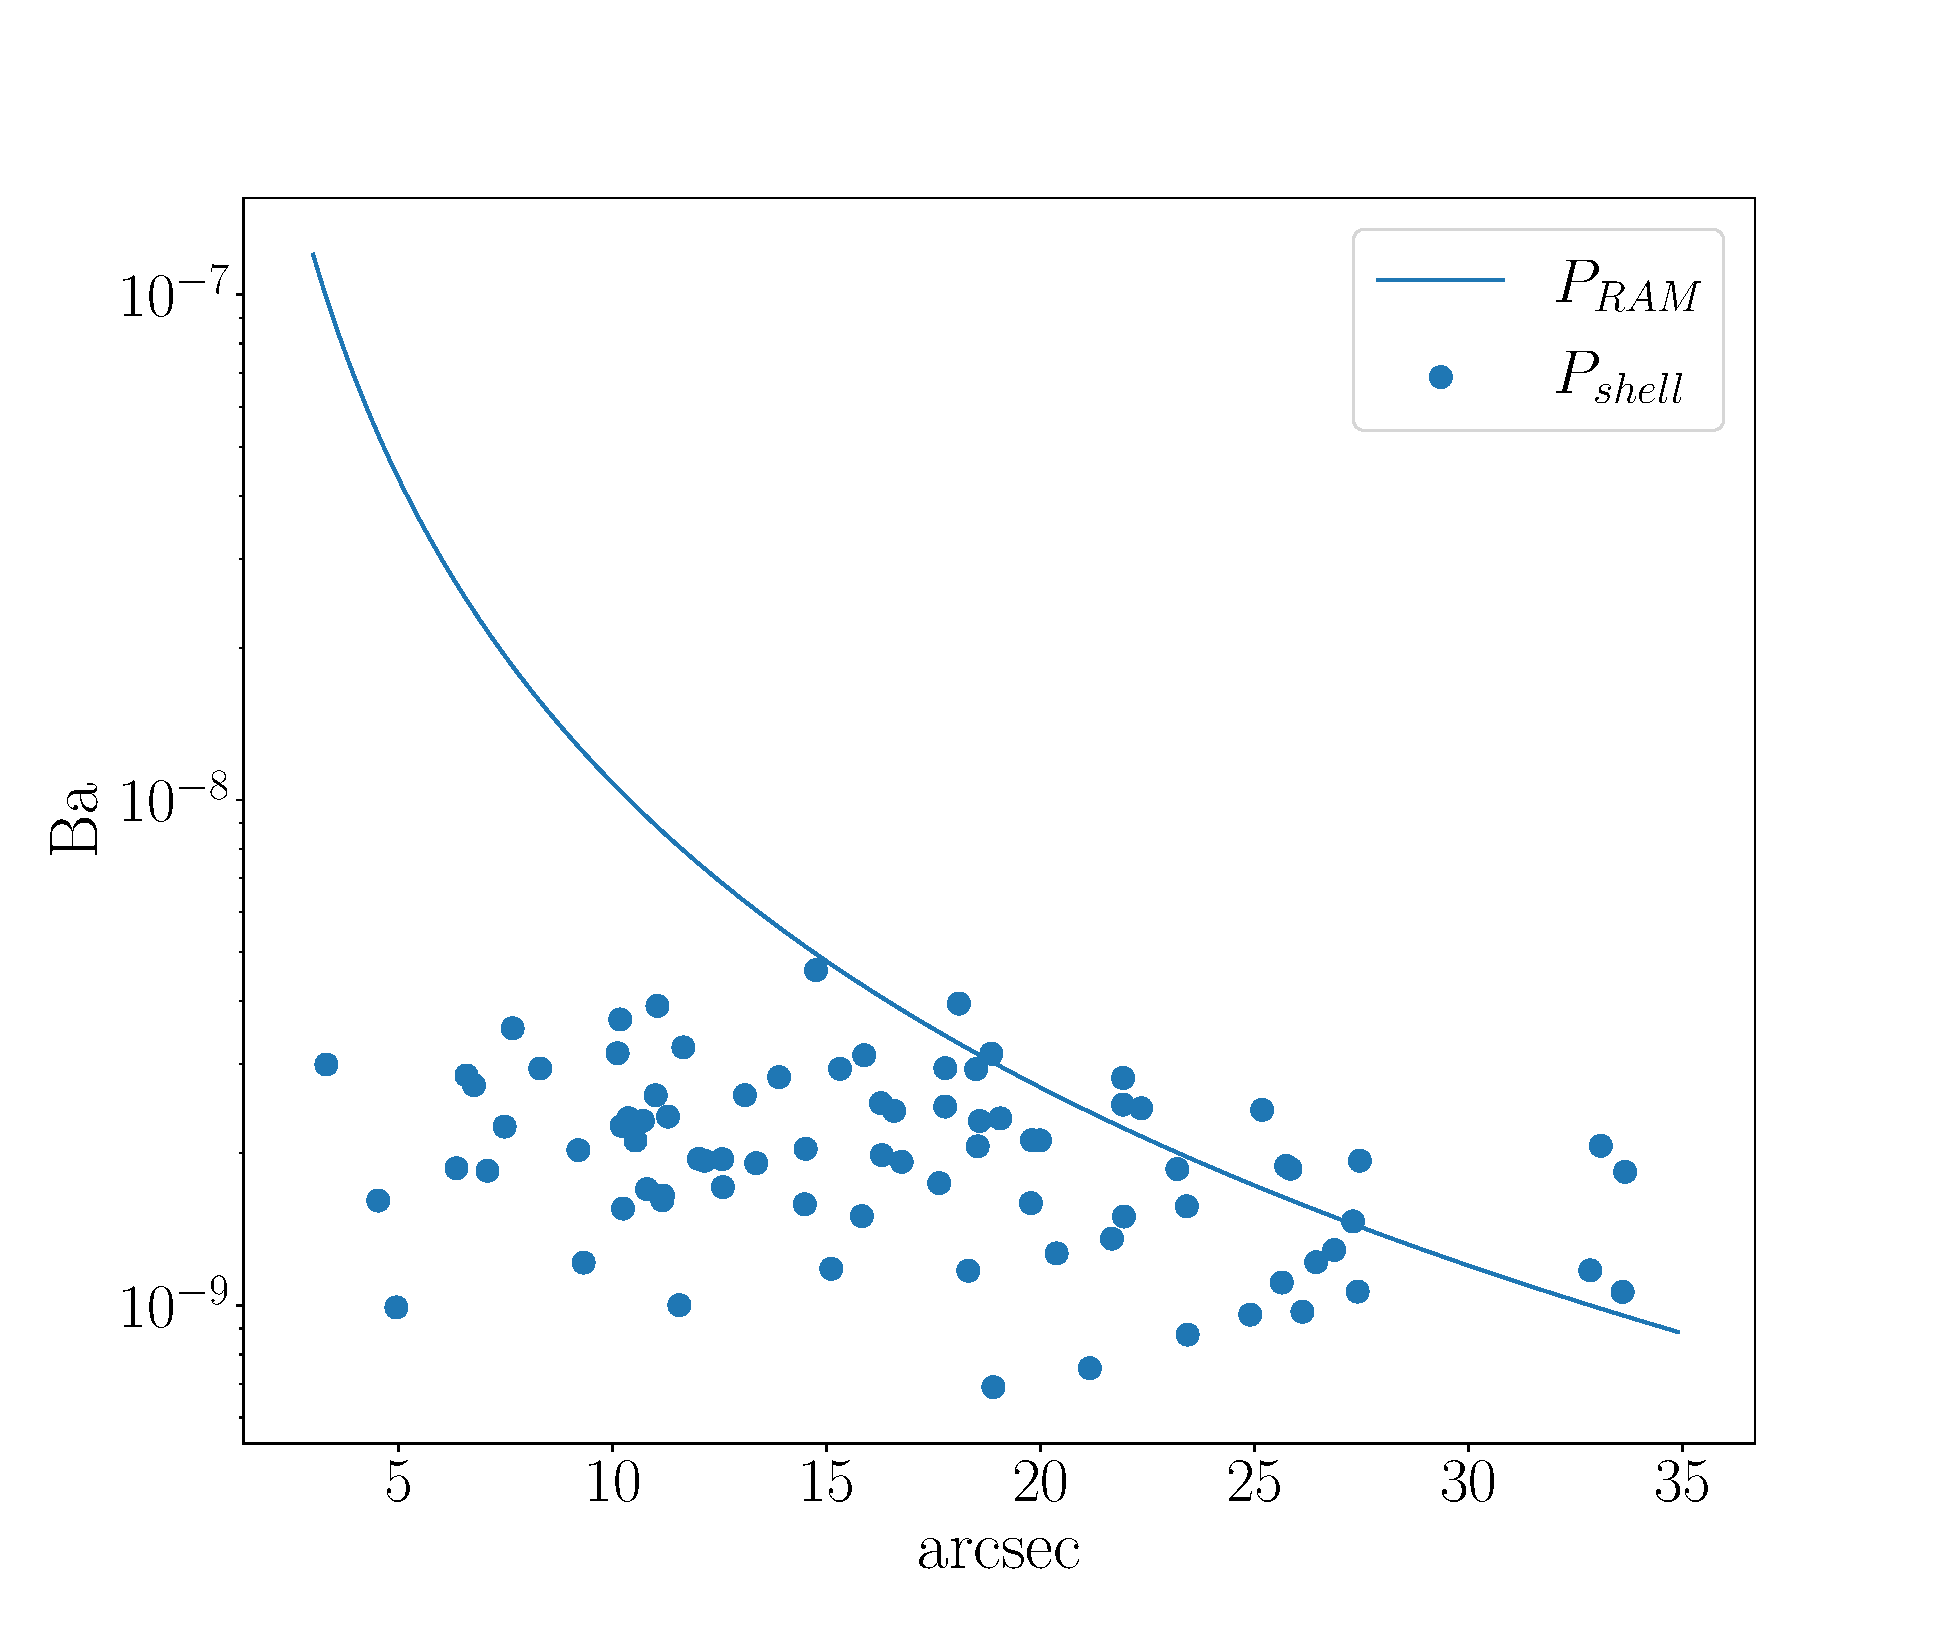
\includegraphics[width=\textwidth]{imagenes Chapter 4/Presiones.pdf}
    \caption{En esta gráfica vemos como las presiones de la cáscara de los glóbulos (círculos azules) está por debajo de la presión RAM (línea azul).}
    \label{graf_presion}
\end{figure}

Si suponemos que el glóbulo está proyectado por un ángulo $i$ como vemos en la figura \ref{Ang proyeccion}, entonces tenemos que \[R\cos i=R_p\] donde $R$ es la separación real del glóbulo a la estrella, $i$ en ángulo de inclinación y $R_p$ la distancia proyecta, que es la que observamos. Como ya habíamos mencionado en la sección \ref{Subsec : EM}, en esta proyección estamos tomando que la densidad también se ve afectada por un factor de $\cos^{1/2}i$.  Por lo que \[P_{g}(i)=\frac{\dot{M}v_\infty}{4\pi R_p^2}\cos{i}^{5/2}\]

\begin{figure}[h]
    \centering
    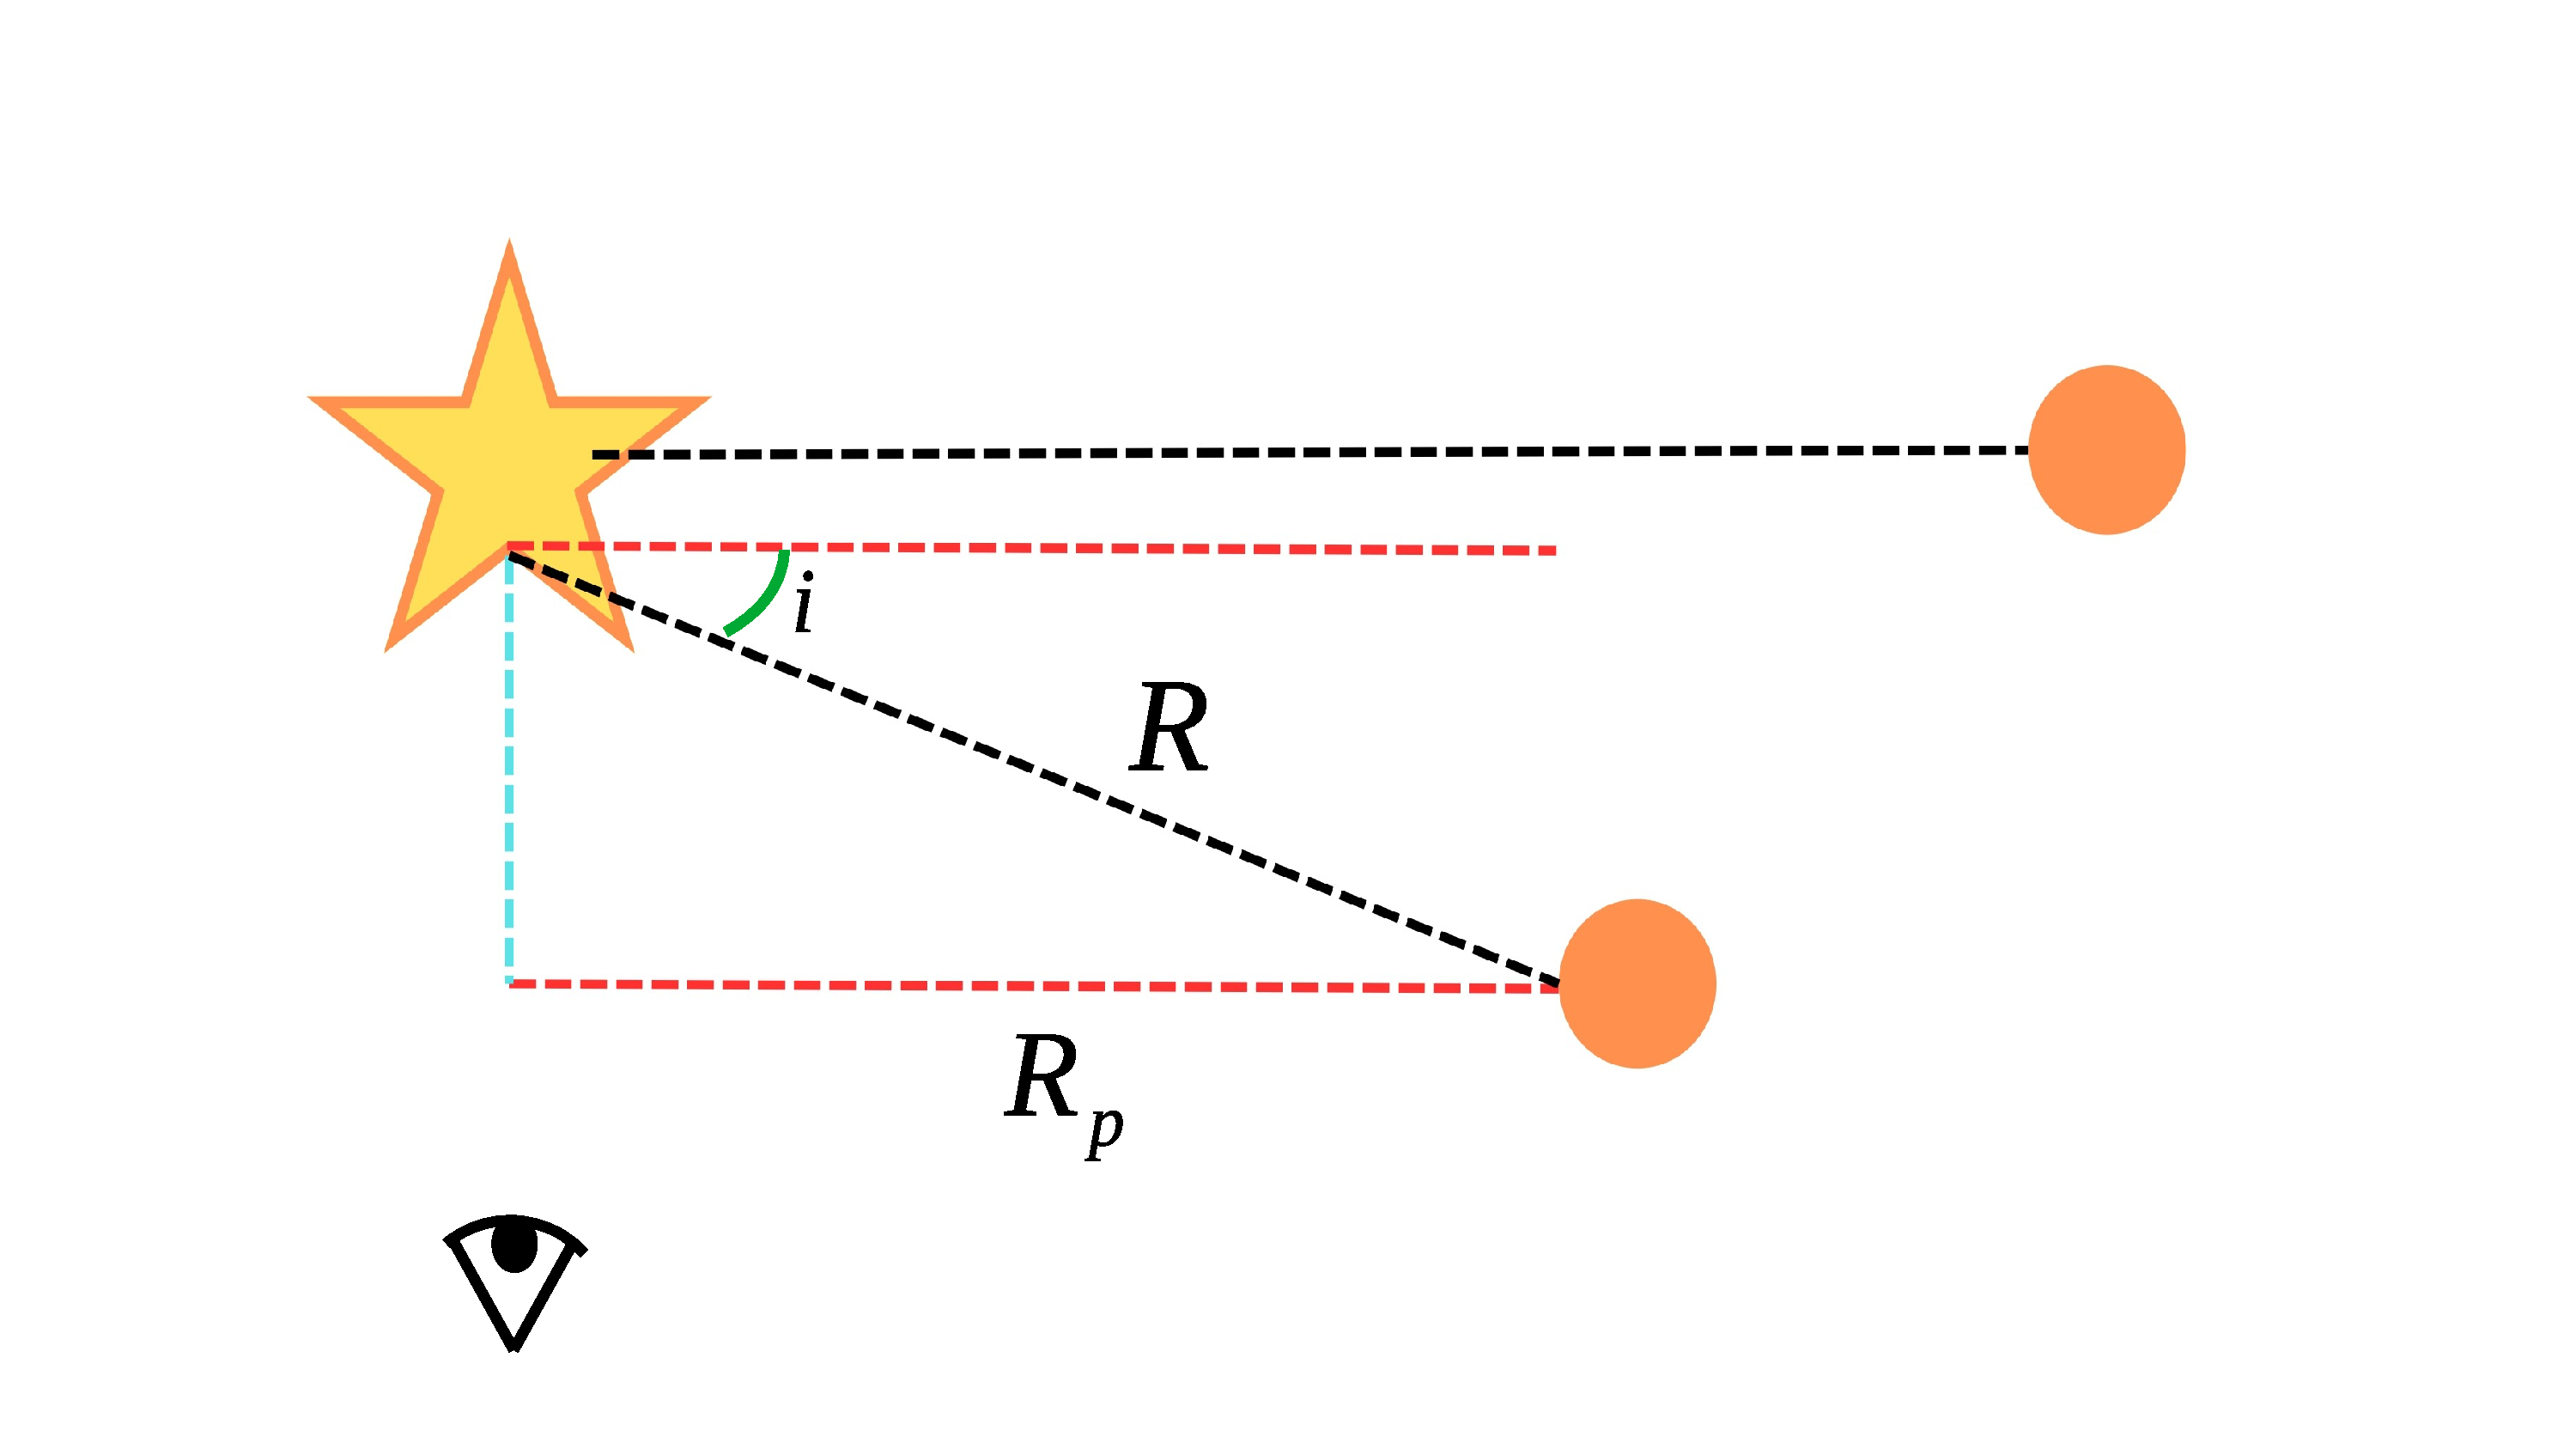
\includegraphics[width=\textwidth]{artesanales/ImgFi01-6.pdf}
    \caption{Representación de como algunos glóbulos se ven afectados por un ángulo de inclinación con respecto a nuestra línea de visión. Para el glóbulo de abajo tenemos que la distancia real a la estrella es $R$, mientras que nosotros vemos $R_p$ que es la distancia proyectada a un ángulo $i$. Por otro lado el glóbulo de arriba no se ve afectado por alguna proyección.}
    \label{Ang proyeccion}
\end{figure}

De esta manera podríamos conocer el ángulo de inclinación de los glóbulos como vemos en la figura \ref{graf_presion_ang}.

\begin{figure}[h]
    \centering
    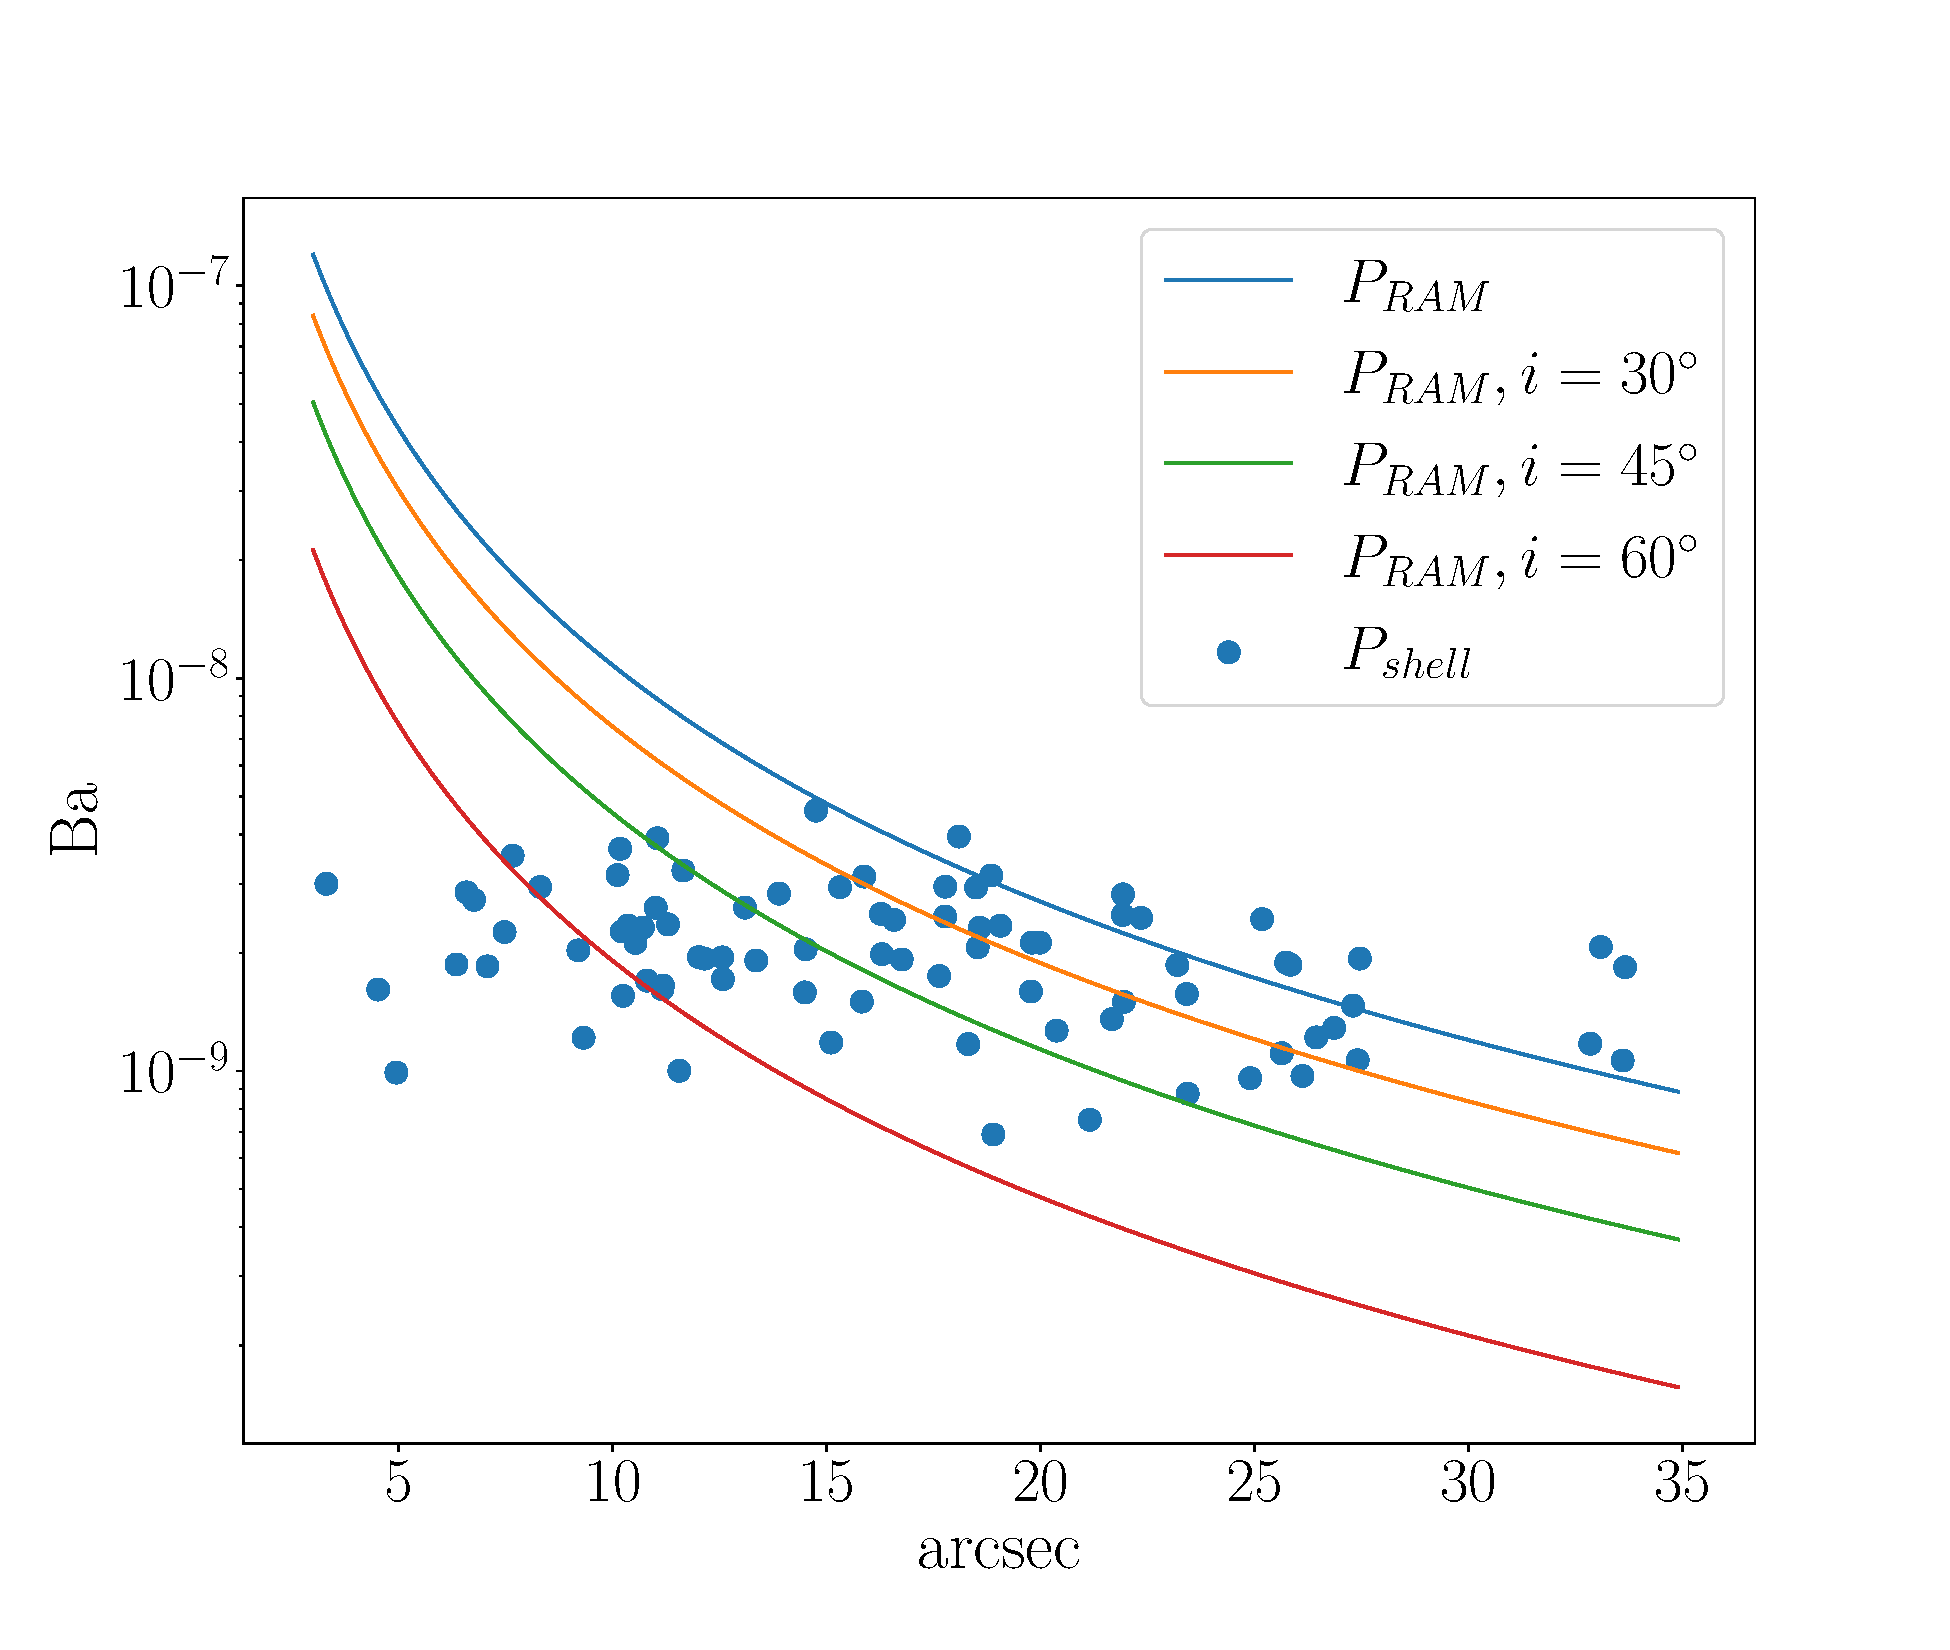
\includegraphics[width=\textwidth]{imagenes Chapter 4/Presiones_ang.pdf}
    \caption{Ahora podemos ver como la presión de la cáscara de los glóbulos (círculos azules) es igual a la presión RAM (líneas continuas) si consideramos cierto ángulo de inclinación.}
    \label{graf_presion_ang}
\end{figure}

Considerando este ángulo de inclinación encontramos que están a un ángulo de inclinación $i$ típico de \SI{40}{^\circ} y que podrían estar alrededor de un radio de \SI{17.54}{\arcsecond} como vemos en la tabla \ref{tab:mean_i} 

\begin{table}[h]
    \centering
    \begin{tabular}{c c c}
        \toprule
        \multicolumn{3}{c}{Resultados con ángulo de inclinación} \\ \midrule
          & Media & Desviación estándar.\\
         cos(i) & 0.78 & 0.29\\
         R & \SI{17.54}{\arcsecond}  & \SI{3.16}{\arcsecond}\\
         $n_{cascara}$ & \SI{1372.15}{cm^{-3}}? & \SI{397.5}{cm^{-3}}? \\
         $P_{g}(i)$ & \SI{3.19e-9}{cgs} & \SI{8.47e-10}{cgs} \\
         \bottomrule
    \end{tabular}
    \caption{Valores típicos de los resultados obtenidos y su desviación estándar considerando el ángulo de inclinación $i$.}
    \label{tab:mean_i}
\end{table}

\section{Comparación con el modelo}

Dadas las observaciones hemos estimado algunos parámetros como sus distintos radio y propiedades sobre todo de la cáscara chocada, pero en nuestro modelos incluye mucho acerca de la parte neutra y la cáscara chocada. 

Ya hemos hecho una medición de los distintos radios, así que ahora vamos a tratar de comparar las presiones entre la parte neutra y la cáscara. 

...



\chapter{Discusión}

Para este caso, \cite{Zavala:2022} estima que la nebulosa planetaria se formó hace unos \SI{11.8}{kyr} por lo que podríamos suponer que las fases mencionadas en la sección \ref{Sec:fluijos fotoevaporativos} ya han pasado y esto es importante porque si estuviéramos en otra fase como en la de implosión, los radios cambiarían además que las presiones que consideramos podrían aún no estar en equilibrio. En el caso de no estar aún en el equilibrio de presiones indicaría que esta interacción entre el flujo fotoevaporativo y el viento estelar se formó recientemente.\\

Como ya habíamos mencionado, hay algunos glóbulos que s encuentran en grupo tal como se ve en la figura \ref{globule_group}. En estos casos la detección de la cáscara chocada es un poco difícil por las siguientes razones. En la imagen de arriba de la figura \ref{globule_group} vemos un claro ejemplo de que cuando dos glóbulos estén muy cercanos se pueden confundir con que sea un solo glóbulo, como es el caso de los que están marcados con círculos azules. De esta manera nos podríamos confundir en el tamaño de la parte neutra del glóbulo y sobrestimarla. Detrás de estos glóbulos se encuentran otros dos glóbulos cercanos (marcados con círculos negros), debido a la proyección en el cielo estos parecen estar en la estela de los glóbulos marcados con círculos azules, por lo que en principio no podríamos detectar bien una cáscara chocada. Por otro lado tenemos el glóbulo marcado con un círculo rojo, este glóbulo es más pequeño que los otros que están en el grupo y aparentemente su cáscara chocada está muy cerca del glóbulo pero en realidad esta cáscara parece ser del par de glóbulos marcados con círculos azules. Algo similar pasa con el glóbulo marcado con el círculo verde, el cual aparentemente no tiene una cáscara pero pareciera estar en la cáscara chocada de algún otro glóbulo.

En la imagen inferior de la figura \ref{globule_group} de igual manera vemos un grupo de glóbulos, pero en esta ocasión están lo suficientemente lejos como para no confundir sus respectivas cáscaras. El problema aquí es que ahora las cáscaras están cerca la una de la otra, por lo que la emisión de una afecta a otras. En este ejemplo en particular, vemos que las cáscaras más grandes contaminan a las más pequeñas en cuanto a su emisión.\\

\begin{figure}[h!]
    \centering
    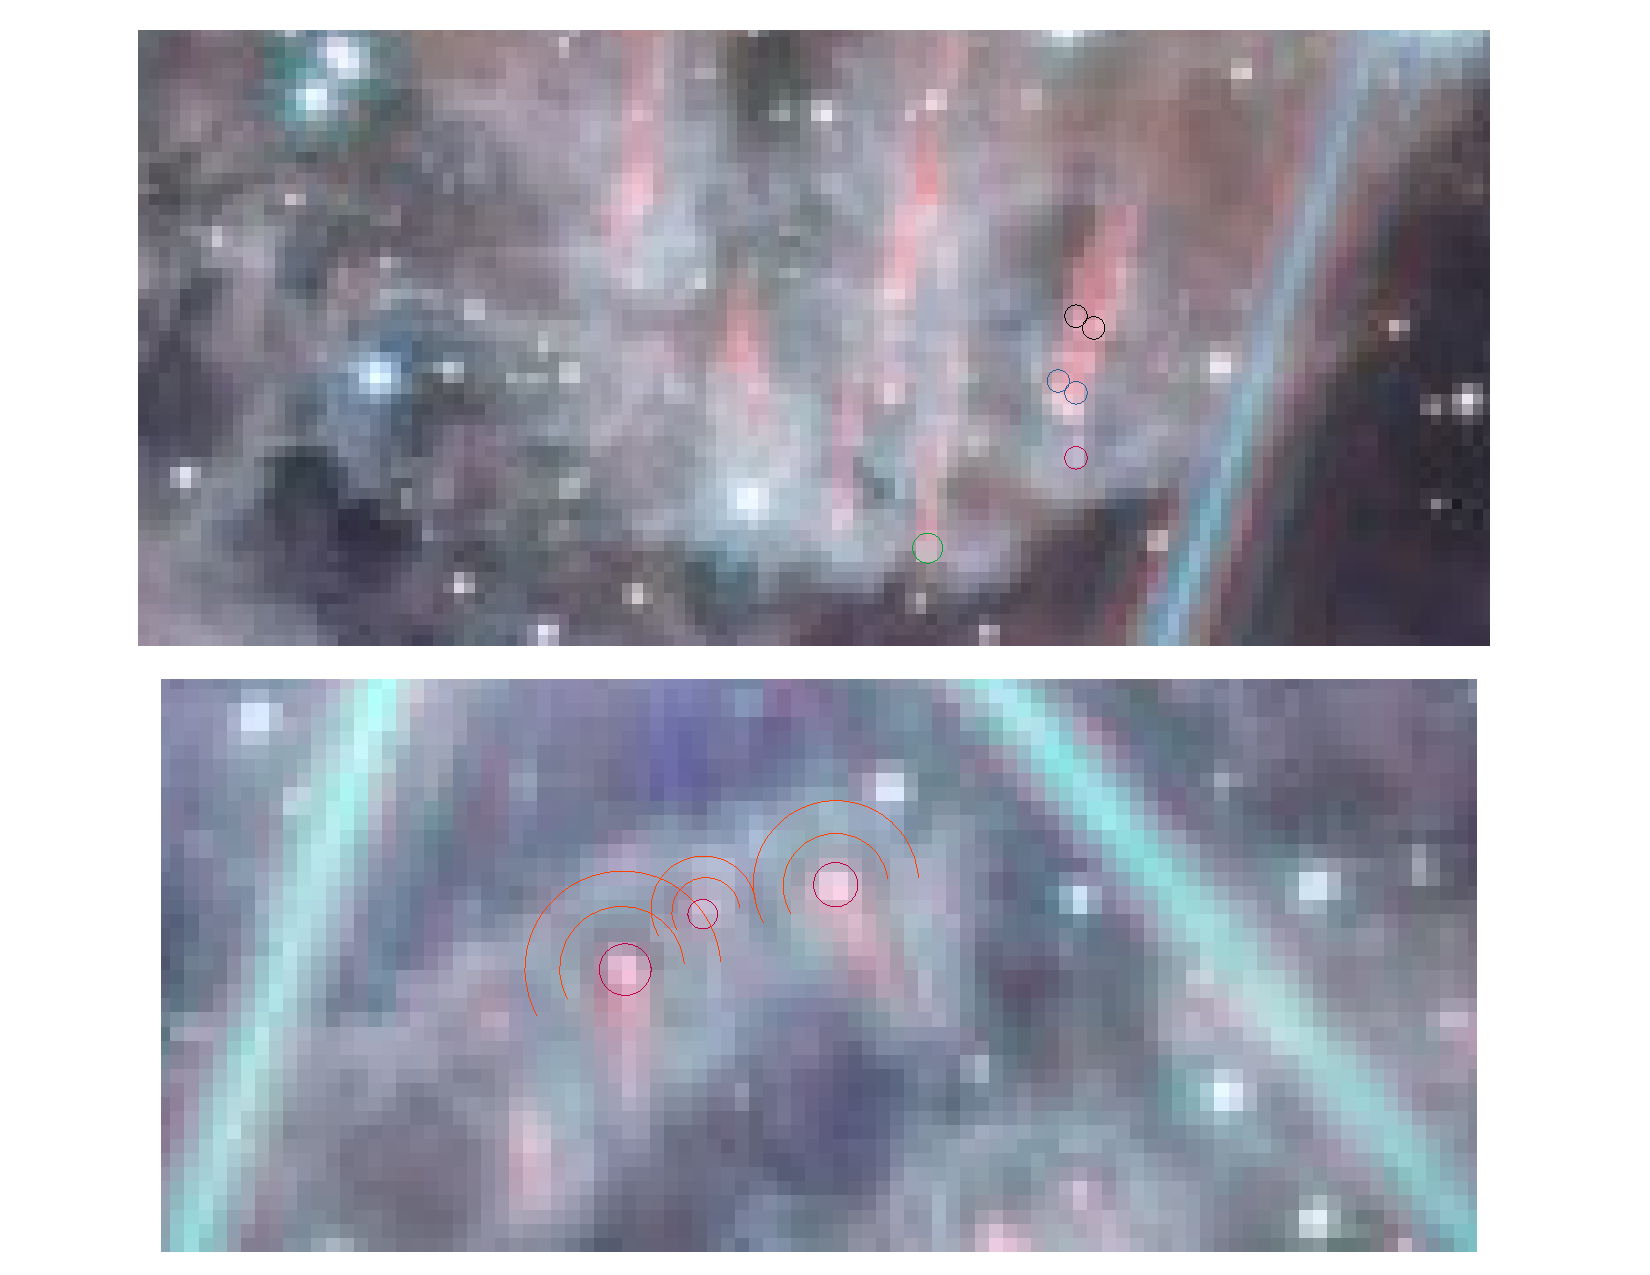
\includegraphics[width=\textwidth]{discusion/groups_globules.pdf}
    \caption{Estos son algunos ejemplos de los grupos de glóbulos que se encontraron en la nebulosa. En la imagen de arriba tenemos varios problemas, entre ellos identificar si es uno o más glóbulos para el caso de los que están muy cerca y saber de qué glóbulo viene cada cáscara chocada, en caso de detectarla. En la imagen de abajo vemos como la cercanía entre glóbulos hace que la emisión de una cáscara chocada se vea afectada por otra cercana.}
    \label{globule_group}
\end{figure}

%Masas y tasa de pérdida de masas 

La corrección por ángulo en principio se puede aplicar solo a los glóbulos cuya presión de la cáscara  es menor que la presión RAM. Si la presión de la cáscara fuera mayor que la presión RAM del viento entonces la cáscara se tendría que expandir hasta encontrar un equilibrio con la presión RAM. Esto en caso de tener un solo glóbulo, pero también podríamos tener un escenario como se muestra en la figura II. En esta figura se ve como la presión RAM primero actúa sobre el glóbulo más cercano a la estrella, en cambio para el otro glóbulo esta presión externa se ve afectada por la interacción anterior. Por lo que la presión RAM no actúa directamente sobre el glóbulo más lejano. Este caso se podría aplicar en algunas estructuras que tenían algunos glóbulos como vemos en la figura III. Estos glóbulos fueron descartados debido a que en la cáscara podría haber material del otro glóbulo y que tendríamos que calcular la presión que actúa sobre ellos ya que la presión RAM se vio afectada por una primer interacción.\\

En esta corrección por ángulo no esperamos ver glóbulos con un ángulo de inclinación de $\pm 90^\circ$ ya que estos estarían totalmente de espaldas o de frente, en cualquier caso estos no los podríamos ver porque se verían afectados por la emisión de la estrella WR ya que en proyección estarían muy cerca de la estrella.

En estas correcciones por proyección se tomó en cuenta que la densidad cae con el ángulo y que en promedio esto decae como $\cos^{1/2}{i}$ (Sección \ref{Sec:proyeccion}). Pero si consideramos que la densidad no decae con el ángulo entonces tendríamos que 
\[P_g(i)= \frac{\dot{M}v_\infty}{4\pi R_p^2}\cos^2 i,\] esto a ángulos pequeños no vemos un gran diferencia pero a grandes ángulos sí, y como vemos en la figura II esto afecta más a los glóbulos que están más cerca de la estrella. 

El modelo propuesto en un principio está puesto para un escenario sencillo, un glóbulo que es radiado por una fuente, pero esto podría ampliarse un poco más si tenemos varias fuentes que radian al glóbulo y una de ellas es la que domina en cuanto al flujo de fotones ionizantes


\chapter{Conclusiones}



\appendix
\chapter{Estimación de fuerzas en el flujo fotoevaporativo ionizado} \label{App:fuerzas}

En estas estimaciones de las diferentes fuerzas solo haremos aproximaciones y para el caso de los valores de los glóbulos usaremos solo los más típicos. Esto ya que los mejores ajustes  tienden a tener a la media en los diferentes valores.

Para comparar las distintas fuerzas es más conveniente comparar las presiones o aceleraciones ya que estas son fuerza por unidad de área o fuerza por unidad de masa, respectivamente. 


Primero vamos a considerar la aceleración provocada por el gradiente de presión, para esto tomamos la fuerza por unidad de masa dad por \[\rho a = \frac{dP}{dr}\Rightarrow a= \frac{1}{\rho}\frac{dP}{dr}=\frac{1}{\rho}\frac{\partial \rho}{\partial r}\frac{\partial P}{\partial\rho}\] como estamos considerando un gas isotermo, vemos que el último término es la velocidad del sonido cuadrada mientras que a los otros términos son la escala de altura $h$, la cual está definida por  \[h^{-1}=\Big|\frac{1}{\rho_0}\frac{\partial\rho}{\partial r}\Big|=\Big|\frac{d \ln \rho}{dr}\Big|\]
usando las ecuaciones de la sección \ref{Estructura} tenemos que \[\frac{\rho}{\rho_0}=e^{\frac{1-M^2}{2}}\Rightarrow\ln\frac{\rho}{\rho_0}=\frac{1-M^2}{2}\]\[\Rightarrow\frac{d\ln\frac{\rho}{\rho_0}}{dM}=-M\] por otro lado usando que \[\frac{r}{r_0}=M^{-1/2}e^{\frac{M^2-1}{2}}\] tenemos que \[d\frac{r}{r_0}=e^{\frac{M^2-1}{4}}\Big(-\frac{M^{-3/2}}{2}+\frac{M}{2M^{1/2}}\Big)dM = \frac{e^{\frac{M^2-1}{4}}}{2}\Big(M^{1/2}-M^{-3/2}\Big)dM\] por lo que \[h^{-1}=\Big|\frac{2M}{e^{\frac{M^2-1}{4}}\Big(M^{1/2}-M^{-3/2}\Big)}\Big|\] que como podemos ver en la fig \ref{fig:h} cerca de $r_0$ tenemos un valor del orden de 0.1. Por lo que el gradiente de presión nos da una aceleración de \[a \approx \frac{c_s^2}{0.1 r_0} = \SI{7.44e-4}{cm.s^{-2}}\] a un radio típico $r_0\sim \SI{0.13}{\arcsecond}$. Como el modelo se resolvió en el eje de simetría, tenemos que aquí los gradientes transversales son cero, mientras que si consideramos el modelo a cierto ángulo debemos considerar que el gradiente de densidad transversal es más pequeño, por un factor de 10 aproximadamente. 

\begin{figure}
    \centering
    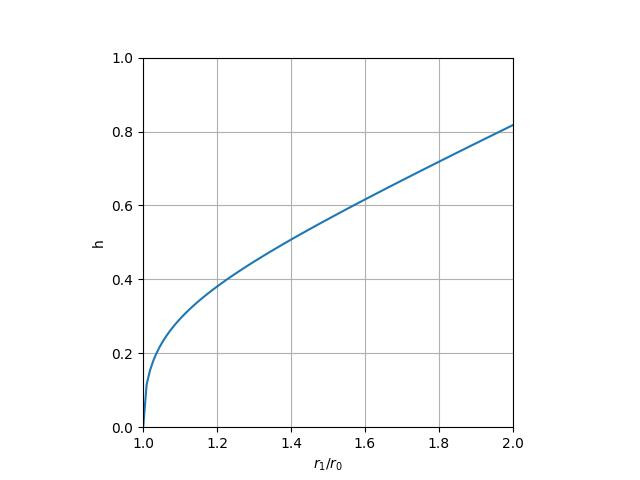
\includegraphics{Appendices/h_3.jpg}
    \caption{Gráfica de $h$ con respecto al radio normalizado. Vemos que cerca de donde tenemos la emisión en $r_0/r_1$ el valor de $h$ es del orden de 0.1}
    \label{fig:h}
\end{figure}

\section{Fuerzas de gravedad} \label{F gravedad}

\cite{Hamann:2019} estima una masa  de 20-$\SI{22}{\msun}$ para la estrella central, por lo que la fuerza de gravedad por parte de la estrella nos da un aceleración de 
\[\frac{GM_*}{r^2}\approx \SI{1.59e-9}{cm/s^2}\] con $r$ una distancia típica entre la estrella y el glóbulo de \SI{16.98}{\arcsecond}

Por parte del glóbulo tenemos una densidad ionizada típica de \SI{1250.46}{cm^{-3}}, un radio $r_0$ típico de \SI{.13}{\arcsecond}, un radio $r_1$ típico de \SI{.54}{\arcsecond} y para la densidad neutra podemos suponer que en la parte neutra domina el campo magnético considerando un balance de presiones. Si aún estuviéramos en la fase de implosión, entonces la densidad sería aún menor. Por lo que usando una velocidad de Alfven tenemos que $\rho_0 = \Big(\frac{c_s}{v_A}\Big)^2\rho_1$, donde $c_s$ es la velocidad del sonido en la parte ionizada y $v_A$ es la velocidad de Alfven que típicamente es de \SI{1}-\SI{3}{km/s}. Para la masa en la parte neutra tenemos que \[M_n = \rho_0 V_0\]
donde $\rho_0$ es la densidad en la parte neutra y $V_0$ es el volumen de la esfera con radio $r_0$, mientras que para la parte ionizada tenemos \[M_i = \rho_1 V_1\] donde $\rho_1$ es a densidad ionizada típica  y $V_1$ es el volumen de la mitad de la cáscara que hay entre $r_0$ y $r_1$, por lo que \[V_1 = \frac{\frac{4}{3}\pi r_1^3-\frac{4}{3}\pi r_0^3}{2}=\frac{2\pi}{3}(r_1^3-r_0^3).\] De esta manera tenemos que la masa total del glóbulo que vamos a considerar en la estimación de esta fuerza es $M_g = M_i + M_n \approx \SI{6.87e-4}{\msun}$ y la aceleración por parte de la fuerza de gravedad del mismo glóbulo es de
\[\frac{G M_g}{r_1^2}\approx \SI{4.6e-11}{cm/s^2}.\] De igual manera podemos despreciar la fuerza de gravedad por parte de los otros glóbulos. 

Estas dos aceleraciones son claramente más pequeñas que la aceleración debido a la diferencia de presiones, por lo que podemos descartar estas fuerzas de gravedad en el modelo.

\section{Presión de radiación}

Estamos considerando que esta presión ya que podemos suponer que todo el momento de los fotones ionizantes se va al flujo fotoevaporativo, por lo que si consideramos que todo la radiación ionizante es absorbida en el flujo fotoevaportivo entonces tememos que para la radiación ionizante $Q = \SI{1.25e49}{s^{-1}}$, según la tabla \ref{tab:parametros WR-124}, tendríamos una intensidad de \[\frac{Q h\nu}{4\pi r^2} = \frac{\SI{2.74e38}{erg.s^{-1}}}{4\pi r^2} \approx \SI{11.48}{erg.s^{-1}.cm^{-s}}\] para la frecuencia de $\SI{1}{Ry}$, el cual es un límite inferior para los fotones que son capaces de ionizar el gas neutro, esto a una distancia típica de los glóbulos. Por lo que tendríamos una presión de radiación de $\approx \SI{3.83e-11}{Pa}$ la cual es una presión menor a la presión RAM del viento estelar o a la presión de los glóbulos.

\chapter{Tiempos de escala}

\section{Tiempo dinámico}

Usando los valores de la tabla \ref{tab:mean}, para el flujo fotoevaporativo tenemos un tiempo dinámico \[t_{DF} = \frac{R_{shell}}{v} \approx \SI{4.73e10}{s}  = \SI{1.49e3}{yr}.\]

Para la nebulosa tenemos un tiempo dinámico de \[t_{DN}= \frac{R_{nebula}}{v_{exp}}\approx\frac{\SI{1.5}{pc}}{\SI{46}{km.s^{-1}}}= \SI{1e12}{s}=\SI{3.17e4}{yr}\]

\section{Tiempo de recombinación}

Usando la densidad promedio de la tabla \ref{tab:mean} tenemos un tiempo de recombinación 
\[t_r = \frac{1}{\alpha_B n} \approx \SI{3.16e9}{s}\]

\chapter{Imágenes de ajustes}

\begin{figure}[h!]
    \centering
    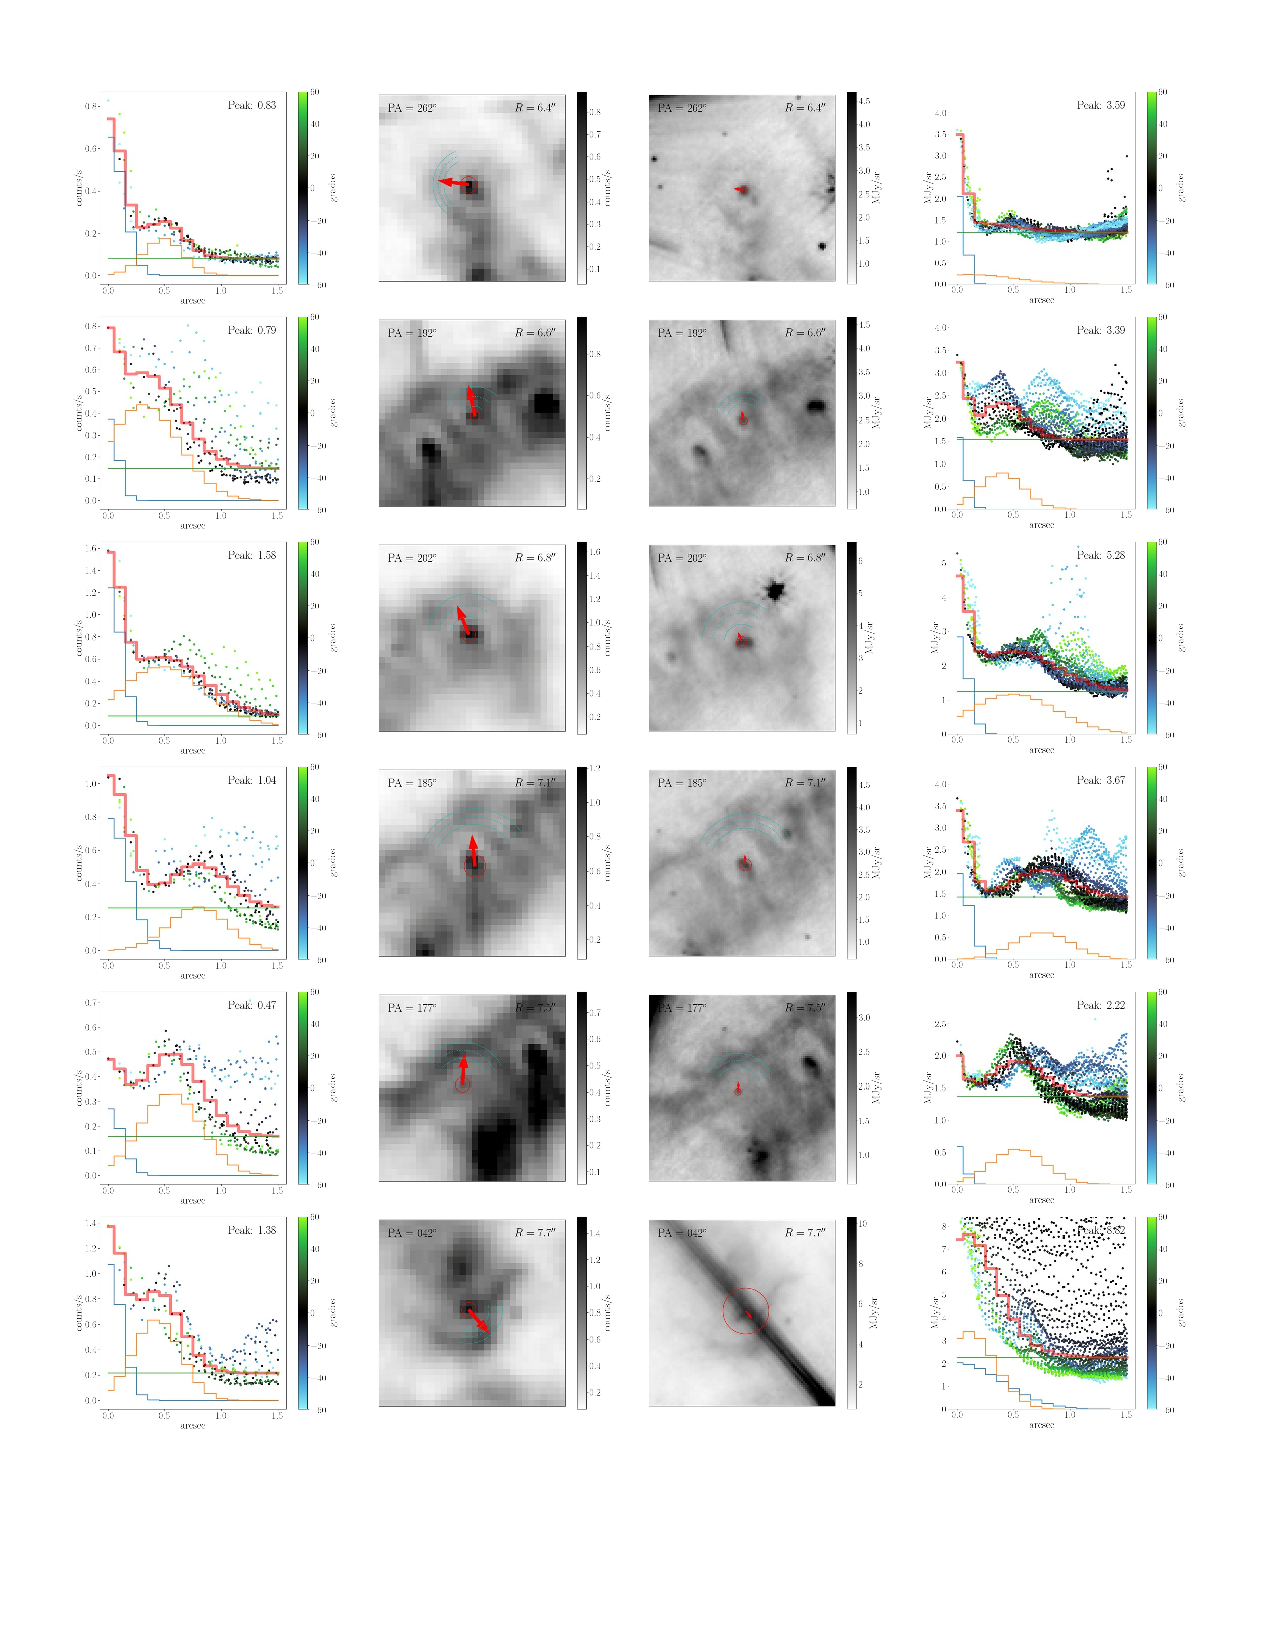
\includegraphics[width=1.2\textwidth]{imagenes Chapter 4/ajustes_075324-1.pdf}
    \caption{Las imágenes del lado izquierdo son con el HST y las de l lado derecho con el JWST. Vemos como el ancho de la cáscara chocada son algo similar en ambas observaciones, mientras que el radio en la parte neutra es más pequeña en las imágenes del JWST.}
    \label{GooG}
\end{figure}
\begin{figure}[h!]
    \centering
    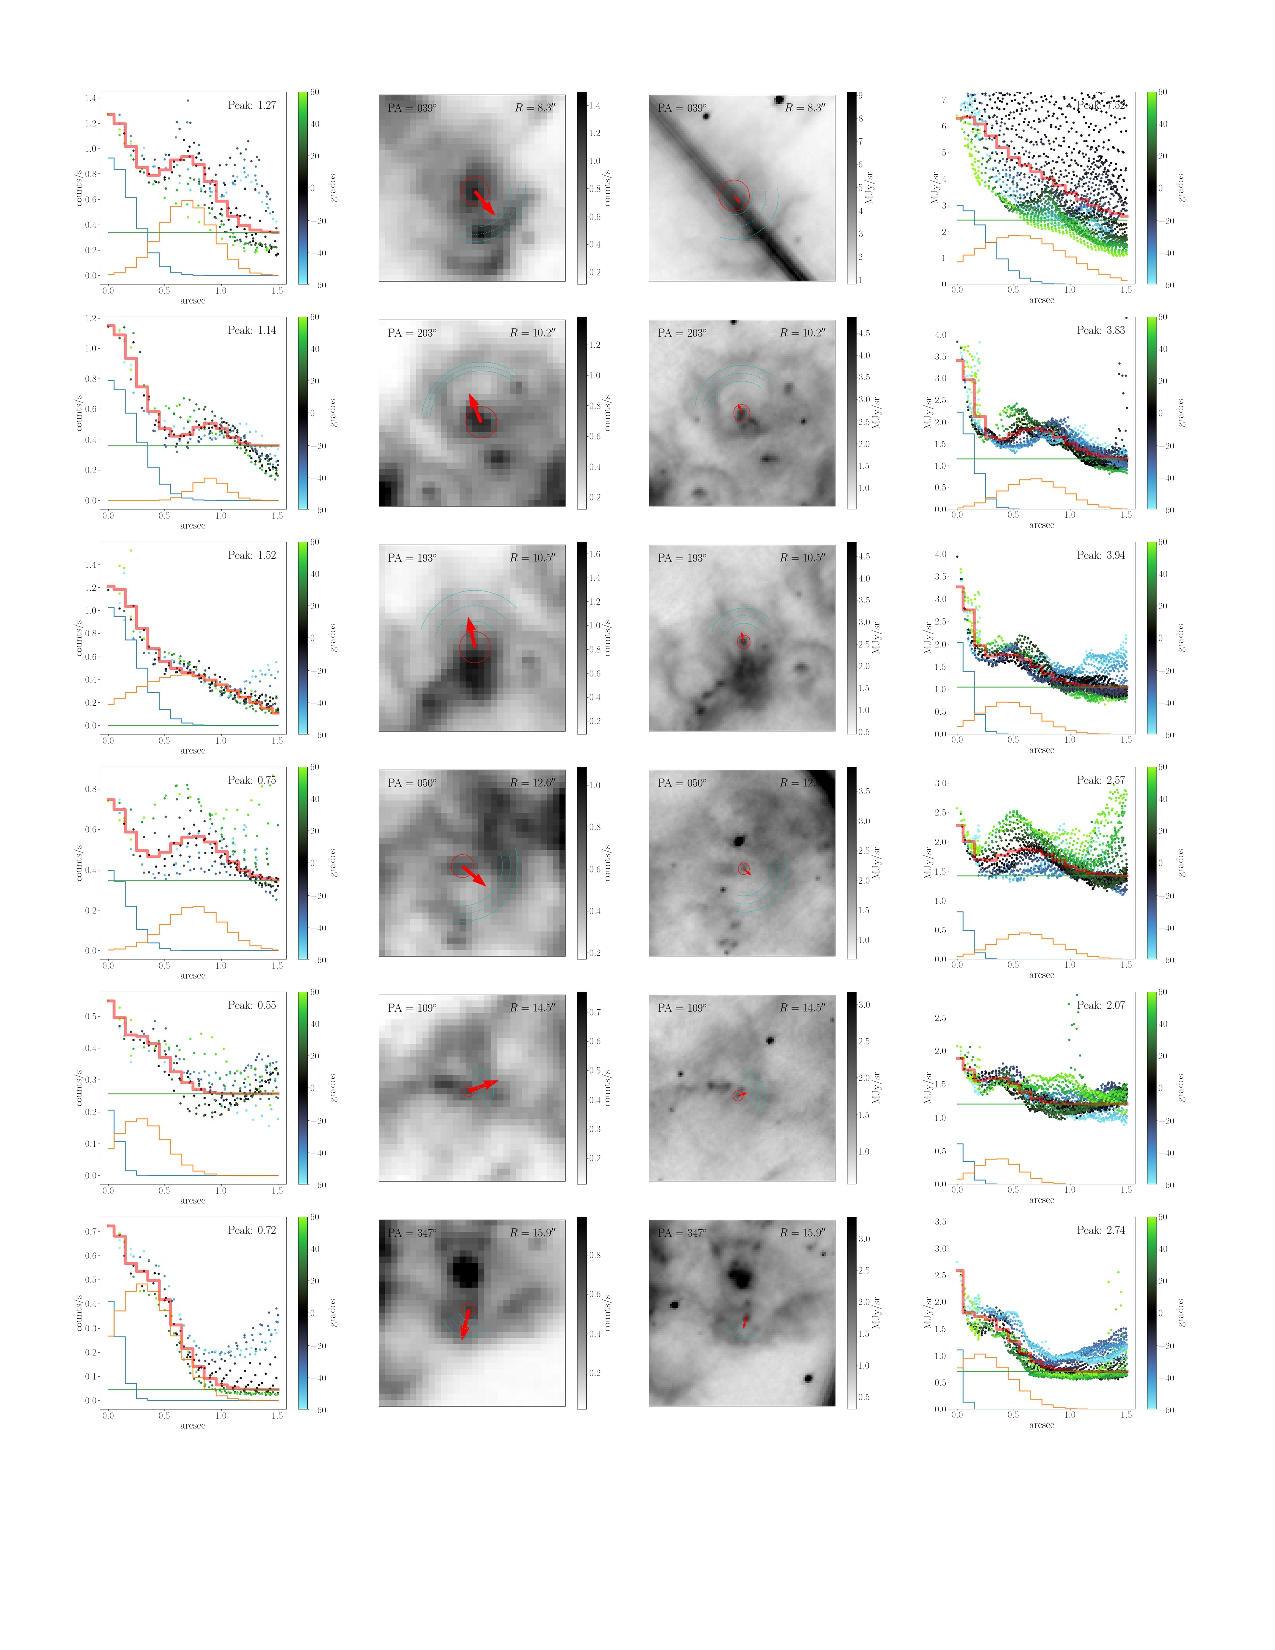
\includegraphics[width=1.2\textwidth]{imagenes Chapter 4/ajustes_075324-2.pdf}
\end{figure}
\begin{figure}[h!]
    \centering
    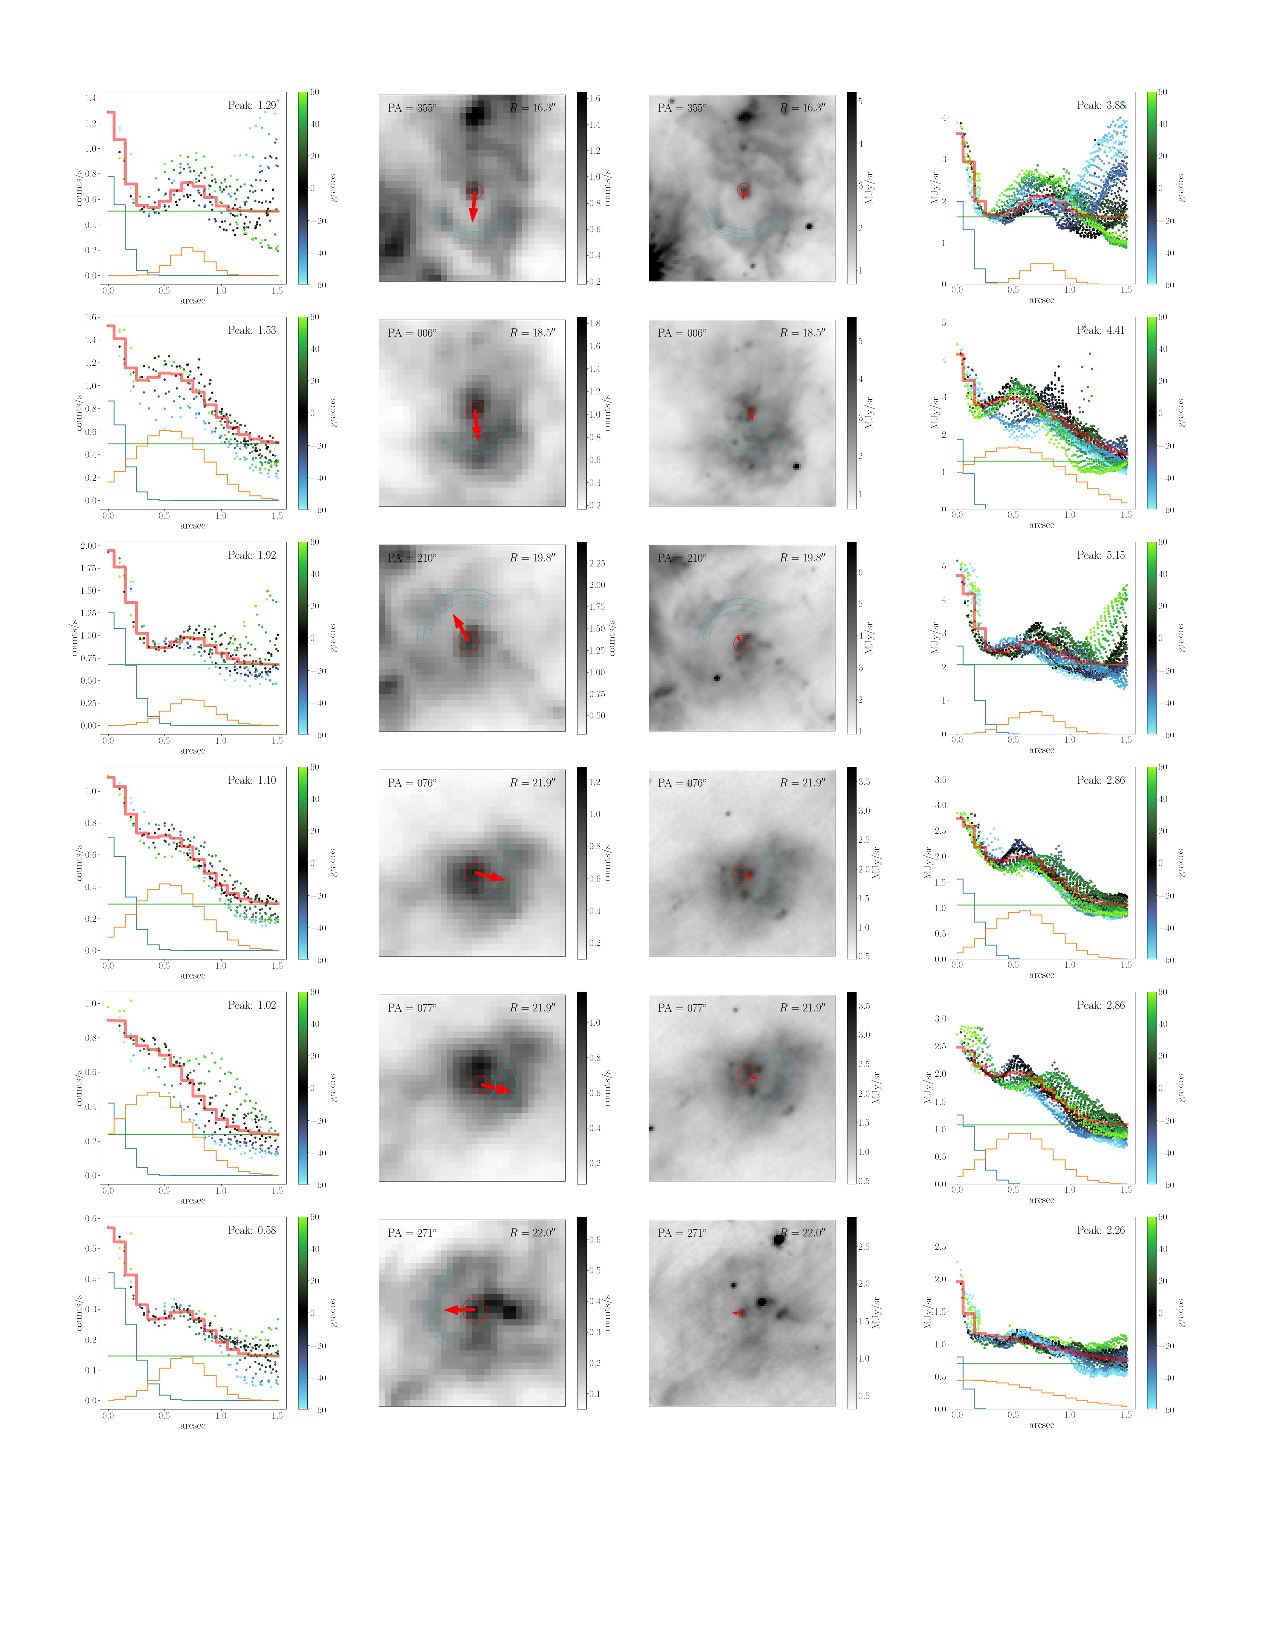
\includegraphics[width=1.2\textwidth]{imagenes Chapter 4/ajustes_075324-3.pdf}
\end{figure}
\begin{figure}[h!]
    \centering
    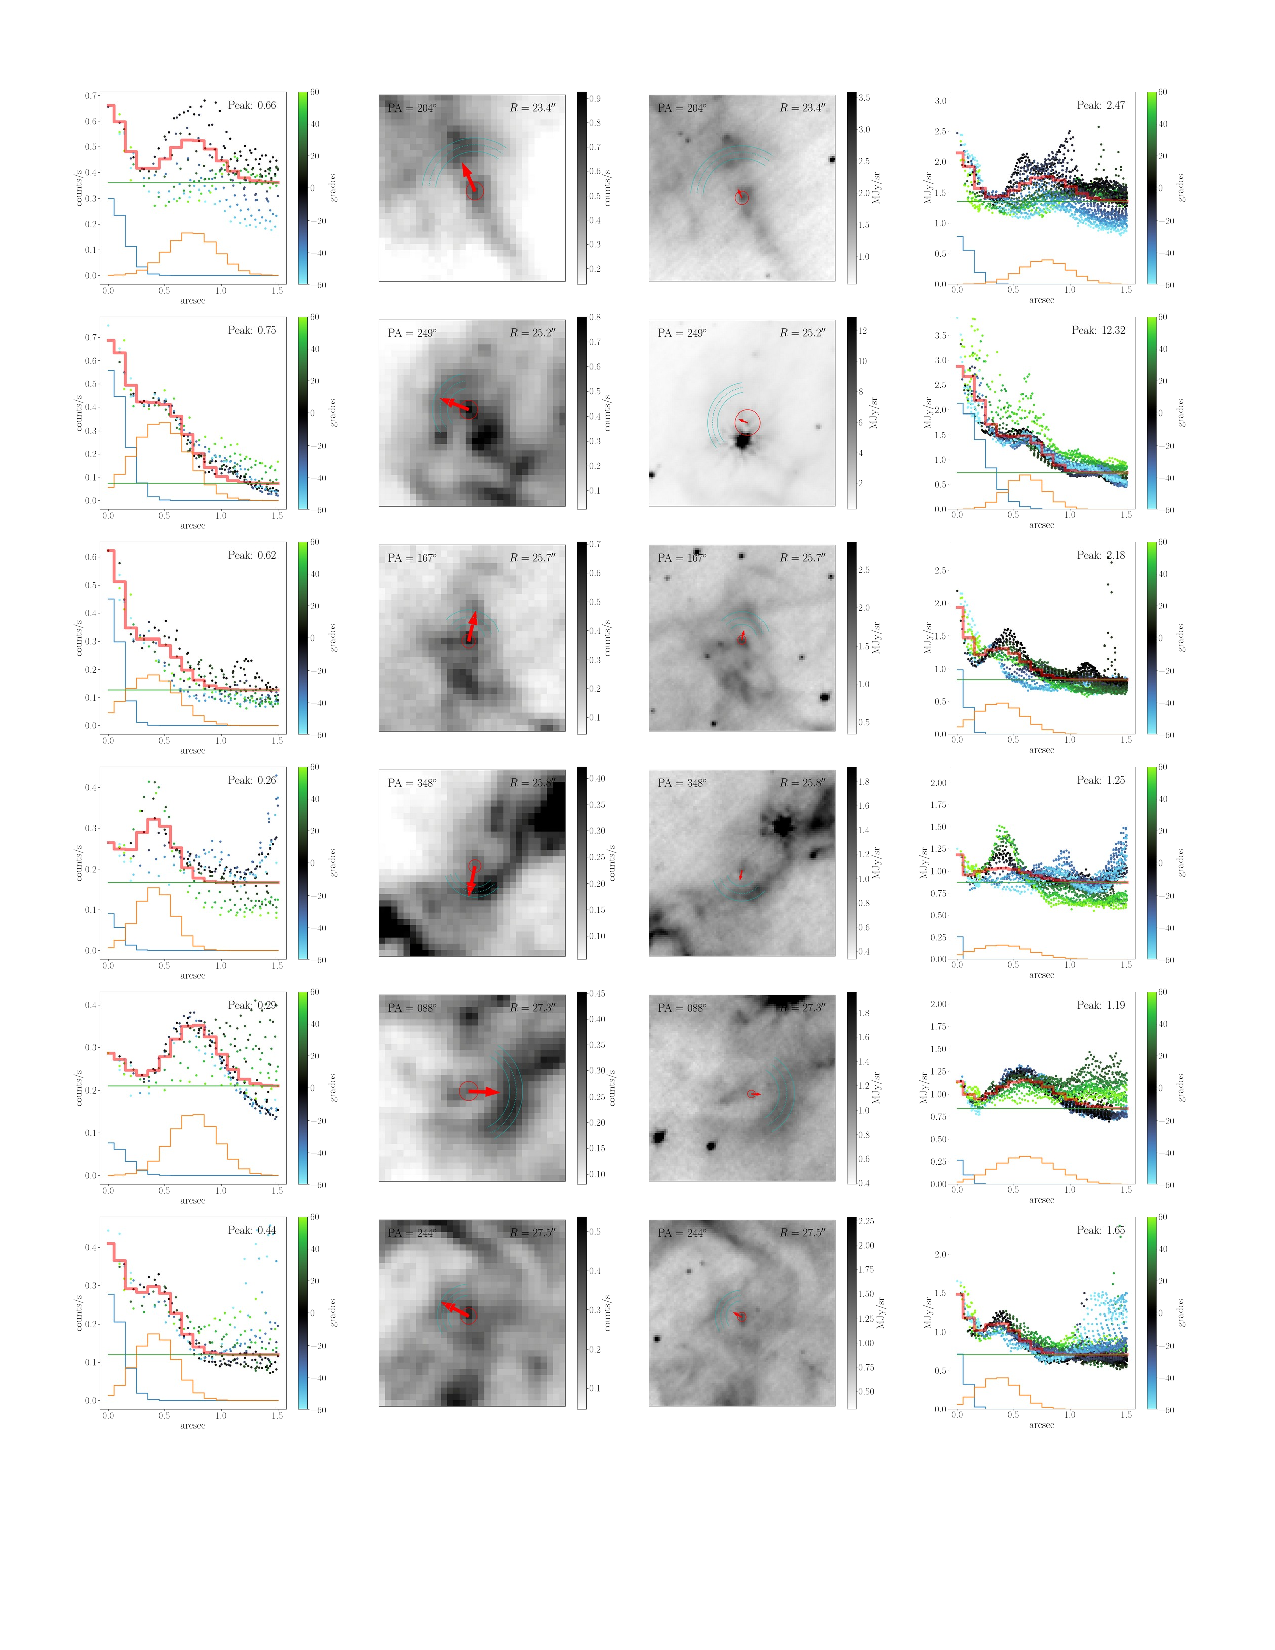
\includegraphics[width=1.2\textwidth]{imagenes Chapter 4/ajustes_075324-4.pdf}
\end{figure}

\bibliography{references}

\end{document}

%%% Local Variables:
%%% mode: LaTeX
%%% TeX-master: t
%%% End:
